%\title{University of Bristol Thesis Template}
\RequirePackage[l2tabu]{nag}		% Warns for incorrect (obsolete) LaTeX usage
%
%
% File: memoirthesis.tex
% Author: Victor Brena
% Description: Contains the thesis template using memoir class,
% which is mainly based on book class but permits better control of 
% chapter styles for example. This template is an adaptation and 
% modification of Oscar's.
% 
% Memoir is a flexible class for typesetting poetry, fiction, 
% non-fiction and mathematical works as books, reports, articles or
% manuscripts. CTAN repository is found at:
% http://www.ctan.org/tex-archive/macros/latex/contrib/memoir/
%
%
% UoB guidelines for thesis presentation were found at:
% http://www.bris.ac.uk/esu/pg/pgrcop11-12topic.pdf#page=49
%
% UoB guidelines:
%
% The dissertation must be printed on A4 white paper. Paper up to A3 may be used
% for maps, plans, diagrams and illustrative material. Pages (apart from the
% preliminary pages) should normally be double-sided.
%
% Memoir class loads useful packages by default (see manual).
\documentclass[a4paper,11pt,reqno,openbib,twoside]{memoir} %add 'draft' to turn draft option on (see below)
%
%
% Adding metadata:
\usepackage{datetime}
\usepackage{ifpdf}
\ifpdf
\pdfinfo{
   /Author (Jan Stocker and Noah H\"utter)
   /Title (Bachelor Thesis)
   /Keywords (FPGA; UDP; Image Processing; Sobel filter)
   /CreationDate (D:\pdfdate)
}
\fi
% When draft option is on. 
\ifdraftdoc 
	\usepackage{draftwatermark}				%Sets watermarks up.
	\SetWatermarkScale{0.3}
	\SetWatermarkText{\bf Draft: \today}
\fi
%
% Declare figure/table as a subfloat.
\newsubfloat{figure}
\newsubfloat{table}
% Better page layout for A4 paper, see memoir manual.
\settrimmedsize{297mm}{210mm}{*}
\setlength{\trimtop}{0pt} 
\setlength{\trimedge}{\stockwidth} 
\addtolength{\trimedge}{-\paperwidth} 
\settypeblocksize{634pt}{448.13pt}{*} 
\setulmargins{4cm}{*}{*} 
\setlrmargins{*}{*}{1.5} 
\setmarginnotes{17pt}{51pt}{\onelineskip} 
\setheadfoot{\onelineskip}{2\onelineskip} 
\setheaderspaces{*}{2\onelineskip}{*} 
\checkandfixthelayout
\setlength{\parindent}{0ex} % Set paragraph indentation
%
\frenchspacing
% Font with math support: New Century Schoolbook
\usepackage{fouriernc}
\usepackage[T1]{fontenc}
%
% UoB guidelines:
%
% Text should be in double or 1.5 line spacing, and font size should be
% chosen to ensure clarity and legibility for the main text and for any
% quotations and footnotes. Margins should allow for eventual hard binding.
%
% Note: This is automatically set by memoir class. Nevertheless \OnehalfSpacing 
% enables double spacing but leaves single spaced for captions for instance. 
\OnehalfSpacing 
%
% Sets numbering division level
\setsecnumdepth{subsection} 
\maxsecnumdepth{subsubsection}
%
% Chapter style (taken and slightly modified from Lars Madsen Memoir Chapter 
% Styles document
\usepackage{calc,soul,fourier}
\makeatletter 
\newlength\dlf@normtxtw 
\setlength\dlf@normtxtw{\textwidth} 
\newsavebox{\feline@chapter} 
\newcommand\feline@chapter@marker[1][4cm]{%
	\sbox\feline@chapter{% 
		\resizebox{!}{#1}{\fboxsep=1pt%
			\colorbox{gray}{\color{white}\thechapter}% 
		}}%
		\rotatebox{90}{% 
			\resizebox{%
				\heightof{\usebox{\feline@chapter}}+\depthof{\usebox{\feline@chapter}}}% 
			{!}{\scshape\so\@chapapp}}\quad%
		\raisebox{\depthof{\usebox{\feline@chapter}}}{\usebox{\feline@chapter}}%
} 
\newcommand\feline@chm[1][4cm]{%
	\sbox\feline@chapter{\feline@chapter@marker[#1]}% 
	\makebox[0pt][c]{% aka \rlap
		\makebox[1cm][r]{\usebox\feline@chapter}%
	}}
\makechapterstyle{daleifmodif}{
	\renewcommand\chapnamefont{\normalfont\Large\scshape\raggedleft\so} 
	\renewcommand\chaptitlefont{\normalfont\Large\bfseries\scshape} 
	\renewcommand\chapternamenum{} \renewcommand\printchaptername{} 
	\renewcommand\printchapternum{\null\hfill\feline@chm[2.5cm]\par} 
	\renewcommand\afterchapternum{\par\vskip\midchapskip} 
	\renewcommand\printchaptertitle[1]{\color{gray}\chaptitlefont\raggedleft ##1\par}
} 
% This sets equal page margins albeit two sided document
\setlength\@tempdima       {\paperwidth}
\addtolength\@tempdima     {-\textwidth}
\setlength\oddsidemargin   {.5\@tempdima}
\addtolength\oddsidemargin {-1in}
\setlength\marginparwidth  {.5\@tempdima}
\addtolength\marginparwidth{-\marginparsep}
\addtolength\marginparwidth{-0.8in} % don't know why this isn't .4
\setlength\evensidemargin\oddsidemargin
\makeatother 
\chapterstyle{daleifmodif}


% Page header and footer style
\makepagestyle{myruled}
\makeheadrule {myruled}{\textwidth}{\normalrulethickness}
\makefootrule {myruled}{\textwidth}{\normalrulethickness}{\footruleskip}
\makeevenhead {myruled}{\small\leftmark}{} {}
\makeoddhead {myruled}{}{}{\small\rightmark}
\makeevenfoot {myruled}{}{\thepage} {}
\makeoddfoot {myruled}{}{\thepage} {}
\makeatletter % because of \@chapapp
\makepsmarks {myruled}{
	\nouppercaseheads
	\createmark {chapter} {both} {shownumber}{\@chapapp\ }{. \ }
	% \createmark {section} {both}{nonumber}{} {. \ }
	% \createmark {subsection} {both}{nonumber}{} {. \ }
	% \createmark {subsubsection}{both}{nonumber}{} {. \ }
	\createplainmark {toc} {both} {\contentsname}
	\createplainmark {lof} {both} {\listfigurename}
	\createplainmark {lot} {both} {\listtablename}
	\createplainmark {bib} {both} {\bibname}
	\createplainmark {index} {both} {\indexname}
	\createplainmark {glossary} {both} {\glossaryname}
}
\makeatother
\setsecnumdepth{subsubsection}
\pagestyle{myruled}


%
% Oscar's command (it works):
% Fills blank pages until next odd-numbered page. Used to emulate single-sided
% frontmatter. This will work for title, abstract and declaration. Though the
% contents sections will each start on an odd-numbered page they will
% spill over onto the even-numbered pages if extending beyond one page
% (hopefully, this is ok).
\newcommand{\clearemptydoublepage}{\newpage{\thispagestyle{empty}\cleardoublepage}}
%
%
% Creates indexes for Table of Contents, List of Figures, List of Tables and Index
\makeindex
% \printglossaries below creates a list of abbreviations. \gls and related
% commands are then used throughout the text, so that latex can automatically
% keep track of which abbreviations have already been defined in the text.
%
% The import command enables each chapter tex file to use relative paths when
% accessing supplementary files. For example, to include
% chapters/brewing/images/figure1.png from chapters/brewing/brewing.tex we can
% use
% \includegraphics{images/figure1}
% instead of
% \includegraphics{chapters/brewing/images/figure1}
\usepackage{import}

% Add other packages needed for chapters here. For example:
\usepackage{lipsum}					%Needed to create dummy text
\usepackage{amsfonts} 					%Calls Amer. Math. Soc. (AMS) fonts
\usepackage[centertags]{amsmath}			%Writes maths centred down
\usepackage{stmaryrd}					%New AMS symbols
\usepackage{amssymb}					%Calls AMS symbols
\usepackage{amsthm}					%Calls AMS theorem environment
\usepackage{newlfont}					%Helpful package for fonts and symbols
\usepackage{layouts}					%Layout diagrams
\usepackage{graphicx}					%Calls figure environment
\usepackage{longtable,rotating}			%Long tab environments including rotation. 
\usepackage[applemac]{inputenc}			%Needed to encode non-english characters 
									%directly for mac
\usepackage{colortbl}					%Makes coloured tables
\usepackage{wasysym}					%More math symbols
\usepackage{mathrsfs}					%Even more math symbols
\usepackage{float}						%Helps to place figures, tables, etc. 
\usepackage{verbatim}					%Permits pre-formated text insertion
\usepackage{upgreek }					%Calls other kind of greek alphabet
\usepackage{latexsym}					%Extra symbols
\usepackage[square,numbers,
		     sort&compress]{natbib}		%Calls bibliography commands 
\usepackage{url}						%Supports url commands
\usepackage{etex}						%eTeXÕs extended support for counters
\usepackage{fixltx2e}					%Eliminates some in felicities of the 
									%original LaTeX kernel
\usepackage[spanish,english]{babel}		%For languages characters and hyphenation
\usepackage{color}                    				%Creates coloured text and background
\usepackage[colorlinks=true,
		     allcolors=black]{hyperref}              %Creates hyperlinks in cross references
\usepackage{memhfixc}					%Must be used on memoir document 
									%class after hyperref
\usepackage{enumerate}					%For enumeration counter
\usepackage{footnote}					%For footnotes
\usepackage{microtype}					%Makes pdf look better.
\usepackage{rotfloat}					%For rotating and float environments as tables, 
									%figures, etc. 
\usepackage{alltt}						%LaTeX commands are not disabled in 
\usepackage{setspace}
									%verbatim-like environment
\usepackage[version=0.96]{pgf}			%PGF/TikZ is a tandem of languages for producing vector graphics from a 
\usepackage{tikz,pgfplots}						%geometric/algebraic description.
\usepackage{xcolor}
\usepackage{tabularx}
\usetikzlibrary{arrows,shapes,snakes,
		       automata,backgrounds,
		       petri,topaths,
		       positioning, spy,
		       fit, external ,calc,
		       arrows.meta, patterns}				%To use diverse features from tikz
\pgfdeclarelayer{background}
\pgfdeclarelayer{foreground}
\pgfsetlayers{background,foreground,main}
\tikzset{>=latex}

\usepackage{xintbinhex}
\usepackage{xintexpr}
\usepackage{listings}
\usepackage{color}
\usepackage[toc,nopostdot,style=altlist,nonumberlist]{glossaries}
% \usepackage[toc,style=longheader,nonumberlist]{glossaries}
\makeglossaries
% ==============================================================================
%
%                             Glossary
%
% ==============================================================================
\newglossaryentry{vivadohlx}
{
    name=Vivado HLx,
    description={Xilinx tool used for synthesis, implementation and debugging}
}
\newglossaryentry{ila}
{
    name=integrated logic analyzer (ILA),
    description={Can be configureed to record FPGA internal signals and send to PC}
}
\newglossaryentry{diip}
{
    name=Distributed Image Processing (diip),
    description={Project nickname of the bachelor thesis}
}
\newglossaryentry{rmse}
{
    name=root mean square error (RMSE),
    description={Used as a metric to measure the difference in two images}
}
 
\definecolor{mGreen}{rgb}{0,0.6,0}
\definecolor{mGray}{rgb}{0.5,0.5,0.5}
\definecolor{mPurple}{rgb}{0.58,0,0.82}
\definecolor{backgroundColour}{rgb}{0.95,0.95,0.92}

\lstdefinestyle{CStyle}{
    backgroundcolor=\color{backgroundColour},   
    commentstyle=\color{mGreen},
    keywordstyle=\color{magenta},
    numberstyle=\tiny\color{mGray},
    stringstyle=\color{mPurple},
    basicstyle=\footnotesize,
    breakatwhitespace=false,         
    breaklines=true,                 
    captionpos=b,                    
    keepspaces=true,                 
    numbers=left,                    
    numbersep=5pt,                  
    showspaces=false,                
    showstringspaces=false,
    showtabs=false,                  
    tabsize=2,
    language=C
}

\lstdefinestyle{TextStyle}{
    backgroundcolor=\color{backgroundColour},   
    basicstyle=\footnotesize,
    breakatwhitespace=false,         
    breaklines=false,                 
    captionpos=b,                    
    keepspaces=true,                 
    numbers=left,                    
    % numbersep=5pt,                  
    showspaces=false,                
    showstringspaces=false,
    showtabs=false,                  
    tabsize=2
}

\lstdefinestyle{VHDLStyle}{
    backgroundcolor=\color{backgroundColour},   
    commentstyle=\color{mGreen},
    keywordstyle=\color{magenta},
    numberstyle=\tiny\color{mGray},
    stringstyle=\color{mPurple},
    basicstyle=\footnotesize,
    breakatwhitespace=false,         
    breaklines=true,                 
    captionpos=b,                    
    keepspaces=true,                 
    numbers=left,                    
    numbersep=5pt,                  
    showspaces=false,                
    showstringspaces=false,
    showtabs=false,                  
    tabsize=2,
    language=VHDL
}

\lstdefinestyle{ShellStyle}{
    backgroundcolor=\color{backgroundColour},   
    commentstyle=\color{mGreen},
    keywordstyle=\color{magenta},
    numberstyle=\tiny\color{mGray},
    stringstyle=\color{mPurple},
    basicstyle=\footnotesize,
    breakatwhitespace=false,         
    breaklines=true,                 
    captionpos=b,                    
    keepspaces=true,                 
    numbers=left,                    
    numbersep=5pt,                  
    showspaces=false,                
    showstringspaces=false,
    showtabs=false,                  
    tabsize=2,
    language=bash
}
\lstdefinestyle{TextStyle}{
    backgroundcolor=\color{backgroundColour},   
    commentstyle=\color{mGreen},
    keywordstyle=\color{magenta},
    numberstyle=\tiny\color{mGray},
    stringstyle=\color{mPurple},
    basicstyle=\footnotesize,
    breakatwhitespace=false,         
    breaklines=true,                 
    captionpos=b,                    
    keepspaces=true,                 
    numbers=left,                    
    numbersep=5pt,                  
    showspaces=false,                
    showstringspaces=false,
    showtabs=false,                  
    tabsize=2
}

\usepackage{mathtools}
\DeclarePairedDelimiter\ceil{\lceil}{\rceil}
\DeclarePairedDelimiter\floor{\lfloor}{\rfloor}

% Reduce line skip in itemize env
\let\tempone\itemize
\let\temptwo\enditemize
\renewenvironment{itemize}{\tempone\addtolength{\itemsep}{-0.5\baselineskip}}{\temptwo}

% Reduce line skip in enumerate env
\let\tempone\enumerate
\let\temptwo\endenumerate
\renewenvironment{enumerate}{\tempone\addtolength{\itemsep}{-0.5\baselineskip}}{\temptwo}


\usepackage[colorinlistoftodos,prependcaption]{todonotes}
\usepackage[section]{placeins} 		% This prevents placing floats (therefore also figures) before a section.
\usepackage{tabularx}
\usepackage{adjustbox}
\usepackage[bottom]{footmisc} 	 	% Allows footnotes to be placed below bottom floats
\usepackage{pdfpages}
\usepackage{cellspace, multirow, booktabs}


%							
%Reduce widows  (the last line of a paragraph at the start of a page) and orphans 
% (the first line of paragraph at the end of a page)
\widowpenalty=1000
\clubpenalty=1000
%
% New command definitions for my thesis
%
\newcommand{\keywords}[1]{\par\noindent{\small{\bf Keywords:} #1}} %Defines keywords small section
\newcommand{\parcial}[2]{\frac{\partial#1}{\partial#2}}                             %Defines a partial operator
\newcommand{\vectorr}[1]{\mathbf{#1}}                                                        %Defines a bold vector
\newcommand{\vecol}[2]{\left(                                                                         %Defines a column vector
	\begin{array}{c} 
		\displaystyle#1 \\
		\displaystyle#2
	\end{array}\right)}
\newcommand{\mados}[4]{\left(                                                                       %Defines a 2x2 matrix
	\begin{array}{cc}
		\displaystyle#1 &\displaystyle #2 \\
		\displaystyle#3 & \displaystyle#4
	\end{array}\right)}
\newcommand{\pgftextcircled}[1]{                                                                    %Defines encircled text
    \setbox0=\hbox{#1}%
    \dimen0\wd0%
    \divide\dimen0 by 2%
    \begin{tikzpicture}[baseline=(a.base)]%
        \useasboundingbox (-\the\dimen0,0pt) rectangle (\the\dimen0,1pt);
        \node[circle,draw,outer sep=0pt,inner sep=0.1ex] (a) {#1};
    \end{tikzpicture}
}
\newcommand{\range}[1]{\textnormal{range }#1}                                             %Defines range operator
\newcommand{\innerp}[2]{\left\langle#1,#2\right\rangle}                                 %Defines inner product
\newcommand{\prom}[1]{\left\langle#1\right\rangle}                                         %Defines average operator
\newcommand{\tra}[1]{\textnormal{tra} \: #1}                                                       %Defines trace operator
\newcommand{\sign}[1]{\textnormal{sign\,}#1}                                                   %Defines sign operator
\newcommand{\sech}[1]{\textnormal{sech} #1}                                                  %Defines sech
\newcommand{\diag}[1]{\textnormal{diag} #1}                                                    %Defines diag operator
\newcommand{\arcsech}[1]{\textnormal{arcsech} #1}                                       %Defines arcsech
\newcommand{\arctanh}[1]{\textnormal{arctanh} #1}                                         %Defines arctanh
%Change tombstone symbol
\newcommand{\blackged}{\hfill$\blacksquare$}
\newcommand{\whiteged}{\hfill$\square$}
\newcounter{proofcount}
\renewenvironment{proof}[1][\proofname.]{\par
 \ifnum \theproofcount>0 \pushQED{\whiteged} \else \pushQED{\blackged} \fi%
 \refstepcounter{proofcount}
 \normalfont 
 \trivlist
 \item[\hskip\labelsep
       \itshape
   {\bf\em #1}]\ignorespaces
}{%
 \addtocounter{proofcount}{-1}
 \popQED\endtrivlist
}
%
%
% New definition of square root:
% it renames \sqrt as \oldsqrt
\let\oldsqrt\sqrt
% it defines the new \sqrt in terms of the old one
\def\sqrt{\mathpalette\DHLhksqrt}
\def\DHLhksqrt#1#2{%
\setbox0=\hbox{$#1\oldsqrt{#2\,}$}\dimen0=\ht0
\advance\dimen0-0.2\ht0
\setbox2=\hbox{\vrule height\ht0 depth -\dimen0}%
{\box0\lower0.4pt\box2}}
%
% My caption style
\newcommand{\mycaption}[2][\@empty]{
	\captionnamefont{\scshape} 
	\changecaptionwidth
	\captionwidth{0.9\linewidth}
	\captiondelim{.\:} 
	\indentcaption{0.75cm}
	\captionstyle[\centering]{}
	\setlength{\belowcaptionskip}{10pt}
	\ifx \@empty#1 \caption{#2}\else \caption[#1]{#2}
}
%
% My subcaption style
\newcommand{\mysubcaption}[2][\@empty]{
	\subcaptionsize{\small}
	\hangsubcaption
	\subcaptionlabelfont{\rmfamily}
	\sidecapstyle{\raggedright}
	\setlength{\belowcaptionskip}{10pt}
	\ifx \@empty#1 \subcaption{#2}\else \subcaption[#1]{#2}
}
%
%An initial of the very first character of the content
\usepackage{lettrine}
\newcommand{\initial}[1]{%
	\lettrine[lines=3,lhang=0.33,nindent=0em]{
		\color{gray}
     		{\textsc{#1}}}{}}
% To print roman numbers
\makeatletter
\newcommand*{\rom}[1]{\expandafter\@slowromancap\romannumeral #1@}
\makeatother
%
% Theorem styles used in my thesis
%
\theoremstyle{plain}
\newtheorem{theo}{Theorem}[chapter]
\theoremstyle{plain}
\newtheorem{prop}{Proposition}[chapter]
\theoremstyle{plain}
\theoremstyle{definition}
\newtheorem{dfn}{Definition}[chapter]
\theoremstyle{plain}
\newtheorem{lema}{Lemma}[chapter]
\theoremstyle{plain}
\newtheorem{cor}{Corollary}[chapter]
\theoremstyle{plain}
\newtheorem{resu}{Result}[chapter]
%
% Hyphenation for some words
%
\hyphenation{res-pec-tively}
\hyphenation{mono-ti-ca-lly}
\hyphenation{hypo-the-sis}
\hyphenation{para-me-ters}
\hyphenation{sol-va-bi-li-ty}
%
%

\begin{document}



% ==============================================================================
%
%                            F R O N T M A T T E R
%
% ==============================================================================
\frontmatter
\pagenumbering{roman}

% <<< -------------------------------------------------------------- TITLEPAGE %
\begin{titlingpage}
\begin{SingleSpace}
\calccentering{\unitlength} 
\begin{adjustwidth*}{\unitlength}{-\unitlength}
\vspace*{0mm}
\begin{center}
\rule[0.5ex]{\linewidth}{2pt}\vspace*{-\baselineskip}\vspace*{3.2pt}
\rule[0.5ex]{\linewidth}{1pt}\\[\baselineskip]

{\HUGE Distributed FPGA for enhanced Image Processing }\\[4mm]
{\Large \textit{Bachelor Thesis}}\\

\rule[0.5ex]{\linewidth}{1pt}\vspace*{-\baselineskip}\vspace{3.2pt}
\rule[0.5ex]{\linewidth}{2pt}\\
\vspace{2mm}
{\large By}\\
\vspace{2mm}

{\large\textsc{Noah H\"utter and Jan Stocker}}\\

\vspace{7mm}

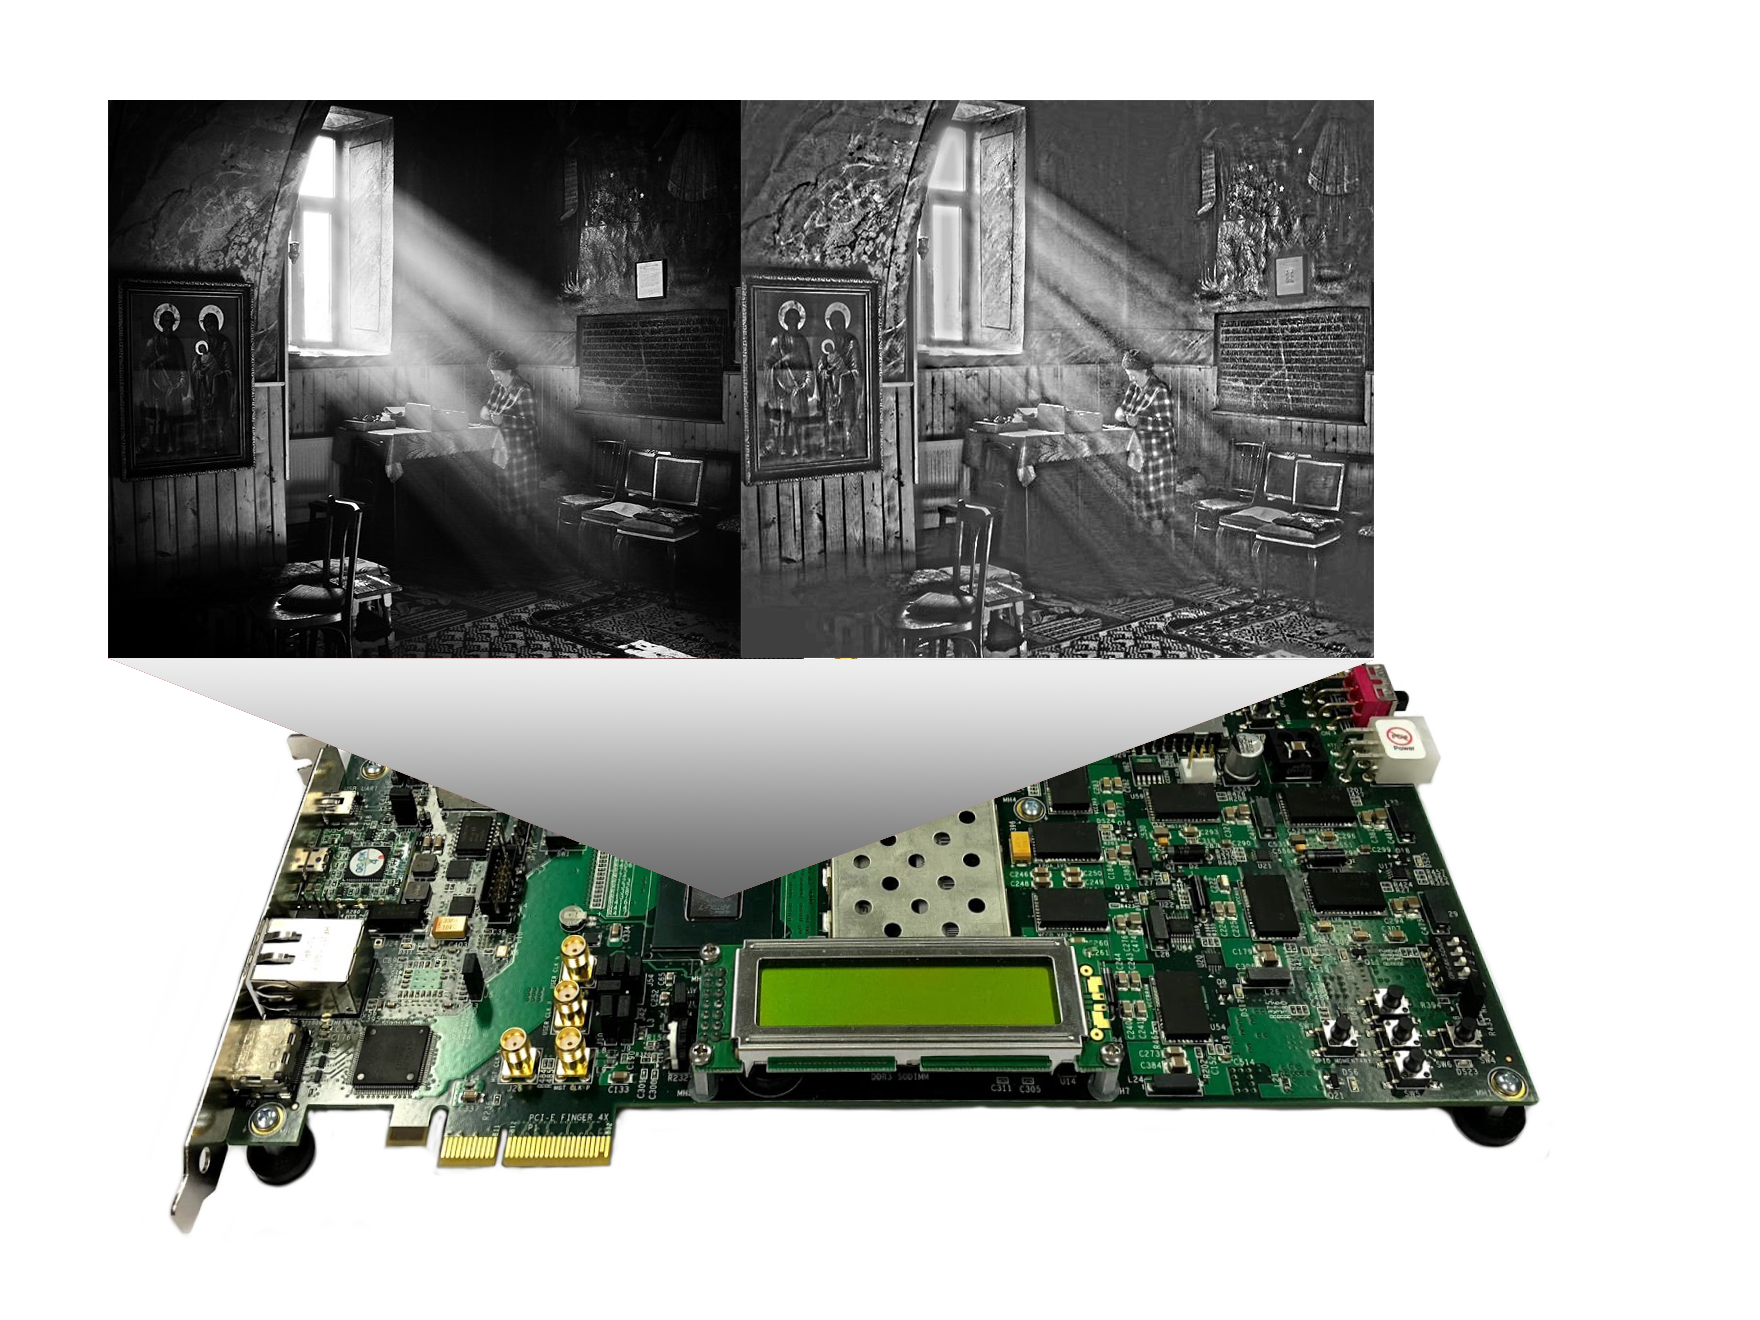
\includegraphics[width=0.88\textwidth]{images/titlepage/p6_titlepage.png}\\

%\vspace{6mm}
%{\large Department of Engineering Mathematics\\
%\textsc{University of Bristol}}\\
\vspace{7mm}

\begin{tabular}{>{\bfseries}rl}
        \large Degree Program   & Electrical and Information Technology \\[2mm]
        \large Coach            & Michael Pichler \\[2mm]
        \large Expert           & Dr. J\"urg M. Stettbacher\\[2mm]
        \large Team             & Noah H\"utter, Jan Stocker \\[2mm]
        \large Date             & \today \\[2mm]
\end{tabular}

%\vspace{9mm}
%{\large\textsc{January 2018}}
\vspace{12mm}
\end{center}
\end{adjustwidth*}
\end{SingleSpace}

\tikzexternaldisable
\begin{tikzpicture}[remember picture,overlay]
    \node[anchor=north east,yshift=-8mm,xshift=-8mm,] 
        at (current page.north east) {
\includegraphics[width=10cm]{images/titlepage/logo-fhnw.pdf}};
\end{tikzpicture}
\tikzexternalenable

\end{titlingpage}

% ------------------------------------------------------------------------->>> %

% <<< ------------------------------------------------------------------- INFO %
% Source
% https://raw.githubusercontent.com/alpenwasser/pitaya/master/doc/report/chunks/info.tex


\vspace*{30mm}

\begin{small}
    \begin{tabular}{lll}
        Content \& Design & \copyright~2018 & Noah H\"utter \\
                          &                  & Jan Stocker  \\
    \end{tabular}


    \vspace{3em}
    \begin{tabular}{p{.9\textwidth}}
        This Bachelor Thesis was created in the spring semester of 2018 at the
        FHNW University of Applied  Sciences and Arts Northwestern Switzerland
        in the degree program \emph{Electrical and Information Technology}.\\
        \\
        \\
    \end{tabular}
    
    \vspace{3em}

    \begin{tabular}{p{.9\textwidth}}
        The code repository to this project is available at\\
        \url{https://gitlab.fhnw.ch/noah.huetter/diip}
        \\
        \\
    \end{tabular}
    \vspace{3em}

    \input{build/revision.tex}
    \begin{tabular}{lp{.9\textwidth}}
        Last compiled on & \compiledate \\
        Based on commit  & \revision \\
        On host          & \hostname \\
        \\
        \\
    \end{tabular}

    \vspace{3em}
    \begin{tabular}{>{\ttfamily}llp{88mm}}
        \textbf{Version History} \\[1ex]
        Version 1.0.0 & June 13, 2018 & Initial Version\\
        Version 1.0.1 & August 10, 2018 & Version for proofreading\\
        Version 1.0.2 & August 13, 2018 & Proofreading completed\\
    \end{tabular}
\end{small}
% ------------------------------------------------------------------------->>> %

% <<< --------------------------------------------------------------- ABSTRACT %
\renewcommand{\abstractname}{Abstract}
{\pagestyle{plain}{
	\setcounter{tocdepth}{2}
	\chapter*{}
\begin{abstract}
% \linespread{2}\selectfont

% % % % % % % % % % % % % % % % % % % % % % % % % % % % % % % % % % % % 
% Motivation:
In the world of self-driving cars and virtual reality games it is becoming
increasingly important to represent digitally what we see.
Therefore, using high resolution
cameras, images of the environment have been recorded.
These large images are processed to be presented three dimensionally. 
% % % % % % % % % % % % % % % % % % % % % % % % % % % % % % % % % % % % 
% Problem statement:
This image processing task needs to be accelerated to get a fast work flow. 
% % % % % % % % % % % % % % % % % % % % % % % % % % % % % % % % % % % % 
% Approach:
A dedicated hardware approach using Field Programmable Gate Arrays (FPGA) was
implemented that is scalable onto multiple FPGAs.
% How
% Using HLS: Wallis and controller
% Using VHDL: Wallis and controller
% 
In a first approach High Level Synthesis was used to describe a Wallis local contrast enhancement filter in C/C++ language that was then synthesized to hardware description language. In order to further improve throughput a VHDL solution was implemented. A memory management unit was introduced to cache necessary image data to reduce Ethernet bandwidth usage.
% High level synthesis was used to describe a Sobel filter operation in
% C language that was then synthesized to hardware description language.
% Simulations were used to ensure correct operation. 
% % % % % % % % % % % % % % % % % % % % % % % % % % % % % % % % % % % % 
% Results:
The result is an image
processing core and a file transfer protocol stack on top of the User Datagram
Protocol (UDP) to transfer the images from a computer to the FPGA over gigabit Ethernet. 
The Wallis filter core processes data at a rate of one
pixel per clock at 125MHz which corresponds to 125 megapixels per second. 
Studies on scalability show how the processing load can be distributed onto multiple FPGA on a local area network and benchmarks present the performance against CPU based image processing.
% The
% code runs on an Xilinx Artix 7 evaluation board and can simply be extended due to a clean source code structure. 
% % % % % % % % % % % % % % % % % % % % % % % % % % % % % % % % % % % % 
% Conclusions:
With some additions, workload distribution is possible. This study proves 
that a dedicated hardware approach for image processing is possible and will
speed up the process of creating virtual representations of reality.

% % % % % % % % % % % % % % % % % % % % % % % % % % % % % % % % % % % % 
\vspace{3em}
\begin{tabular}{l p{.95\textwidth}}
    \textbf{Team members}  & Noah H\"utter, Jan Stocker \\
    \textbf{Keywords}      & FPGA, UDP, Image Processing, Wallis Filter \\
\end{tabular}

\end{abstract}

% % % % % % % % % % % % % % % % % % % % % % % % % % % % % % % % % % % % 
% Motivation:
% Why do we care about the problem and the results? If the problem isn't obviously "interesting" it might be better to put motivation first; but if your work is incremental progress on a problem that is widely recognized as important, then it is probably better to put the problem statement first to indicate which piece of the larger problem you are breaking off to work on. This section should include the importance of your work, the difficulty of the area, and the impact it might have if successful.
% 
% Why do we care about the problem? 
% What practical, scientific, theoretical or artistic gap is your research filling?
% 
% 
% % % % % % % % % % % % % % % % % % % % % % % % % % % % % % % % % % % % 
% Problem statement:
% What problem are you trying to solve? What is the scope of your work (a generalized approach, or for a specific situation)? Be careful not to use too much jargon. In some cases it is appropriate to put the problem statement before the motivation, but usually this only works if most readers already understand why the problem is important.
% 
% % % % % % % % % % % % % % % % % % % % % % % % % % % % % % % % % % % % 
% Approach:
% How did you go about solving or making progress on the problem? Did you use simulation, analytic models, prototype construction, or analysis of field data for an actual product? What was the extent of your work (did you look at one application program or a hundred programs in twenty different programming languages?) What important variables did you control, ignore, or measure?

% % % % % % % % % % % % % % % % % % % % % % % % % % % % % % % % % % % % 
% Results:
% What's the answer? Specifically, most good computer architecture papers conclude that something is so many percent faster, cheaper, smaller, or otherwise better than something else. Put the result there, in numbers. Avoid vague, hand-waving results such as "very", "small", or "significant." If you must be vague, you are only given license to do so when you can talk about orders-of-magnitude improvement. There is a tension here in that you should not provide numbers that can be easily misinterpreted, but on the other hand you don't have room for all the caveats.

% % % % % % % % % % % % % % % % % % % % % % % % % % % % % % % % % % % % 
% Conclusions:
% What are the implications of your answer? Is it going to change the world (unlikely), be a significant "win", be a nice hack, or simply serve as a road sign indicating that this path is a waste of time (all of the previous results are useful). Are your results general, potentially generalizable, or specific to a particular case?
% 
% https://users.ece.cmu.edu/~koopman/essays/abstract.html
}}
% \chapter*{}
\begin{abstract}
% \linespread{2}\selectfont

% % % % % % % % % % % % % % % % % % % % % % % % % % % % % % % % % % % % 
% Motivation:
In the world of self-driving cars and virtual reality games it is becoming
increasingly important to represent digitally what we see.
Therefore, using high resolution
cameras, images of the environment have been recorded.
These large images are processed to be presented three dimensionally. 
% % % % % % % % % % % % % % % % % % % % % % % % % % % % % % % % % % % % 
% Problem statement:
This image processing task needs to be accelerated to get a fast work flow. 
% % % % % % % % % % % % % % % % % % % % % % % % % % % % % % % % % % % % 
% Approach:
A dedicated hardware approach using Field Programmable Gate Arrays (FPGA) was
implemented that is scalable onto multiple FPGAs.
% How
% Using HLS: Wallis and controller
% Using VHDL: Wallis and controller
% 
In a first approach High Level Synthesis was used to describe a Wallis local contrast enhancement filter in C/C++ language that was then synthesized to hardware description language. In order to further improve throughput a VHDL solution was implemented. A memory management unit was introduced to cache necessary image data to reduce Ethernet bandwidth usage.
% High level synthesis was used to describe a Sobel filter operation in
% C language that was then synthesized to hardware description language.
% Simulations were used to ensure correct operation. 
% % % % % % % % % % % % % % % % % % % % % % % % % % % % % % % % % % % % 
% Results:
The result is an image
processing core and a file transfer protocol stack on top of the User Datagram
Protocol (UDP) to transfer the images from a computer to the FPGA over gigabit Ethernet. 
The Wallis filter core processes data at a rate of one
pixel per clock at 125MHz which corresponds to 125 megapixels per second. 
Studies on scalability show how the processing load can be distributed onto multiple FPGA on a local area network and benchmarks present the performance against CPU based image processing.
% The
% code runs on an Xilinx Artix 7 evaluation board and can simply be extended due to a clean source code structure. 
% % % % % % % % % % % % % % % % % % % % % % % % % % % % % % % % % % % % 
% Conclusions:
With some additions, workload distribution is possible. This study proves 
that a dedicated hardware approach for image processing is possible and will
speed up the process of creating virtual representations of reality.

% % % % % % % % % % % % % % % % % % % % % % % % % % % % % % % % % % % % 
\vspace{3em}
\begin{tabular}{l p{.95\textwidth}}
    \textbf{Team members}  & Noah H\"utter, Jan Stocker \\
    \textbf{Keywords}      & FPGA, UDP, Image Processing, Wallis Filter \\
\end{tabular}

\end{abstract}

% % % % % % % % % % % % % % % % % % % % % % % % % % % % % % % % % % % % 
% Motivation:
% Why do we care about the problem and the results? If the problem isn't obviously "interesting" it might be better to put motivation first; but if your work is incremental progress on a problem that is widely recognized as important, then it is probably better to put the problem statement first to indicate which piece of the larger problem you are breaking off to work on. This section should include the importance of your work, the difficulty of the area, and the impact it might have if successful.
% 
% Why do we care about the problem? 
% What practical, scientific, theoretical or artistic gap is your research filling?
% 
% 
% % % % % % % % % % % % % % % % % % % % % % % % % % % % % % % % % % % % 
% Problem statement:
% What problem are you trying to solve? What is the scope of your work (a generalized approach, or for a specific situation)? Be careful not to use too much jargon. In some cases it is appropriate to put the problem statement before the motivation, but usually this only works if most readers already understand why the problem is important.
% 
% % % % % % % % % % % % % % % % % % % % % % % % % % % % % % % % % % % % 
% Approach:
% How did you go about solving or making progress on the problem? Did you use simulation, analytic models, prototype construction, or analysis of field data for an actual product? What was the extent of your work (did you look at one application program or a hundred programs in twenty different programming languages?) What important variables did you control, ignore, or measure?

% % % % % % % % % % % % % % % % % % % % % % % % % % % % % % % % % % % % 
% Results:
% What's the answer? Specifically, most good computer architecture papers conclude that something is so many percent faster, cheaper, smaller, or otherwise better than something else. Put the result there, in numbers. Avoid vague, hand-waving results such as "very", "small", or "significant." If you must be vague, you are only given license to do so when you can talk about orders-of-magnitude improvement. There is a tension here in that you should not provide numbers that can be easily misinterpreted, but on the other hand you don't have room for all the caveats.

% % % % % % % % % % % % % % % % % % % % % % % % % % % % % % % % % % % % 
% Conclusions:
% What are the implications of your answer? Is it going to change the world (unlikely), be a significant "win", be a nice hack, or simply serve as a road sign indicating that this path is a waste of time (all of the previous results are useful). Are your results general, potentially generalizable, or specific to a particular case?
% 
% https://users.ece.cmu.edu/~koopman/essays/abstract.html

\pagestyle{plain}
\renewcommand{\chaptermark}[1]{\markboth{#1}{}}


%

\chapter*{Dedication and acknowledgements}
\begin{SingleSpace}
\todo[inline]{Fill that stuff}
% We wish to express our sincere thanks to ..., Principal of the Faculty, for
% providing us with all the necessary facilities for the research.
% \\

% We place on record, our sincere thank you to ... Dean of the Faculty, for the
% continuos encouragement.
% \\

% We are also grateful to ..., lecturer, in the Department of .... We are extremly
% thankful and indebted to him for sharing expertise, sincere and valuable
% guidance and encouragement extended to us.
% \\

% We take this opportunity to express gratitude to all of the Department faculty
% members for their help and support. We also thank our parents for the unceasing
% encouragement, support and attention.


We wish to express our sincere thanks to those who supported us in completing
this Thesis. With technical support from the guys at Nomoko, in particular Hakki
and
Luc, the implementation of the Wallis filter became possible. We are
grateful to Michael Pichler, lecturer and Thesis coach, for providing us with
his profound knowledge in FPGA development. 
\\

Further, we would like to place on record, our sincere thanks to the people who
have made themselves available for proofreading our work. In terms of spelling
and reading flow, Tabea Berger and Anita Gertiser provided us with their
thoughts on the text. The feedback from Thomas H\"utter and Dino Zardet helped
us phrase the findings and our line of thought in a comprehensible manner.


% Gegenlesen
% - Anita Gertiser
% - Tabea Berger
% - Thomas H\"utter
% - Dino Zardet
%
% Technische Unterstützung
% - Michael Pichler
% - Luc, Hakki from Nomoko for image processing
%
%

 \end{SingleSpace} \clearpage
\clearemptydoublepage
%
\chapter*{Author's declaration}
\begin{SingleSpace}
\begin{quote}
\todo[inline]{Verify text}
We declare that the work in this thesis was carried out in accordance with
the requirements of  the University's Regulations and Code of Practice for
Research Degree Programmes and that it  has not been submitted for any other
academic award. Except where indicated by specific  reference in the text, the
work is the candidate's own work. Work done in collaboration with, or with the
assistance of, others, is indicated as such. Any views expressed in the
thesis are those of the authors.

\vspace{3cm}

\begin{table}[h!]
    \centering
    \begin{tabular}{p{5cm} p{3cm} p{5cm}}
         & & \\ \cline{1-1} \cline{3-3} 
        \vspace{1ex} & & \\
        \multicolumn{1}{c}{Noah H\"utter} &
        August 17, 2018
         & \multicolumn{1}{c}{Jan Stocker} \\
    \end{tabular}
\end{table}

% \vspace{2cm}
% \noindent
% \hspace{-0.75cm}
% \textsc{SIGNED: ....................................................
% DATE: ..........................................}
% Noah H\"utter


% \vspace{1.5cm}
% \noindent
% \hspace{-0.75cm}
% \textsc{SIGNED: ....................................................
% DATE: ..........................................}
% Jan Stocker

\end{quote}
\end{SingleSpace}
\clearpage
\clearemptydoublepage
%


\newpage
% ------------------------------------------------------------------------->>> %

% <<< ------------------------------------------------------ TABLE of CONTENTS %
{\pagestyle{plain}{
\setcounter{tocdepth}{2}
\begin{KeepFromToc} % remove TOC from TOC
  \tableofcontents
\end{KeepFromToc}
%}}

\pagestyle{plain}
%\pagenumbering{arabic}
\renewcommand{\chaptermark}[1]{\markboth{#1}{}}
% ------------------------------------------------------------------------->>> %




% ==============================================================================
%
%                             M A I N M A T T E R
%
% ==============================================================================
\mainmatter
\pagestyle{myruled}
% <<< ----------------------------------------------------------- INTRODUCTION %

% ==============================================================================
%
%                             Introduction
%
% ==============================================================================
\chapter{Introduction}
% Field/Context
Self driving cars are getting more popular and virtual reality video games
increasingly find their way into people's living rooms. One thing they share is
the need for a digital copy of the world. Self driving cars are trained in such
worlds to
accelerate the development of the algorithm and virtual reality games are
becoming more realistic. The Zurich based company Nomoko \cite{nomoko} is developing a
technology that will enable the creation of digital copies of the world. They
built a giga pixel camera and a 3D image processing pipeline to make this happen. This pipeline
consists among other things of high volume image processing. Modern computers
and graphical processing units (GPU) are fast in sequentially processing data
but are designed to serve many different tasks and not a specific one. A
dedicated hardware approach designed for a specific image processing task would
expedite the 3D processing pipeline of creating digital copies of the world.
\\

% Project goal/aims
The goal of this project is to implement such an image processing task on a
Field
Programmable Gate Array (FPGA). FPGAs
consist of thousands of logical elements that can be configured and connected
together to form a complex logical operation. Together with on chip
memory they offer high throughput by processing the data in parallel in contrast to
sequential. The data is transfered to the FPGA over an Ethernet LAN connection
for
fast transfer rates. To accelerate the computing even further, the system needs
to be scalable to multiple FPGA boards to distribute the workload.

% Build upon 
In preparation for this thesis, a semester project focused on two building
blocks for this work: The communication block and the image processing block
\cite{p5report}. The results were two seperate parts working but neither
connected nor optimized. This thesis builds upon the results of said work and
focuses on two main goals:

% Primary objectives
\begin{enumerate}
    \item Increase throughput of the dataflow by improving the communication and
    by putting thoughts on scalability
    \item Implement a more complex image processing algorithm to show the real
    benefit of using FPGA for image processing
\end{enumerate}
% \begin{figure}[t!]
%     \centering
%     % \tikzsetnextfilename{system-overview}
\begin{tikzpicture}[
    rounded corners=0mm,
]
    %coordinates
    \coordinate (corig)      at (0,0);
    \coordinate (cmonitor)   at (0,0);
    \coordinate (ccom)       at (5,0);
    \coordinate (cip)        at (10,0);


    %nodes

    \begin{pgfonlayer}{main}
        \node[draw, fill=white, minimum width=3.2cm, minimum height=1.8cm, anchor=west, align=center, rounded corners=1mm] (mon) at (cmonitor) {};

        \node[draw, fill=white, minimum width=2.1cm, minimum height=0.4cm, anchor=west, align=center, rounded corners=2mm, below=0.2cm of mon] (stand) {};
        \node[draw, fill=white, minimum width=0.2cm, minimum height=0.1cm, anchor=south, align=center] (stange) at ($(stand.90) + (0,-0.04)$) {};



        \node[draw, fill=white, minimum width=3cm, minimum height=1cm, anchor=west, text width=2.8cm, align=center, right = 2cm of mon] (com) at (ccom) {Communication};

        \node[draw, fill=white, minimum width=3cm, minimum height=1cm, anchor=west, text width=2.8cm, align=center, right = 1cm of com] (ip) {Image\\Processing};
        

        \node[inner sep=0pt, anchor=west] (whitehead) at ($(cmonitor) + (0.1,0)$)
            {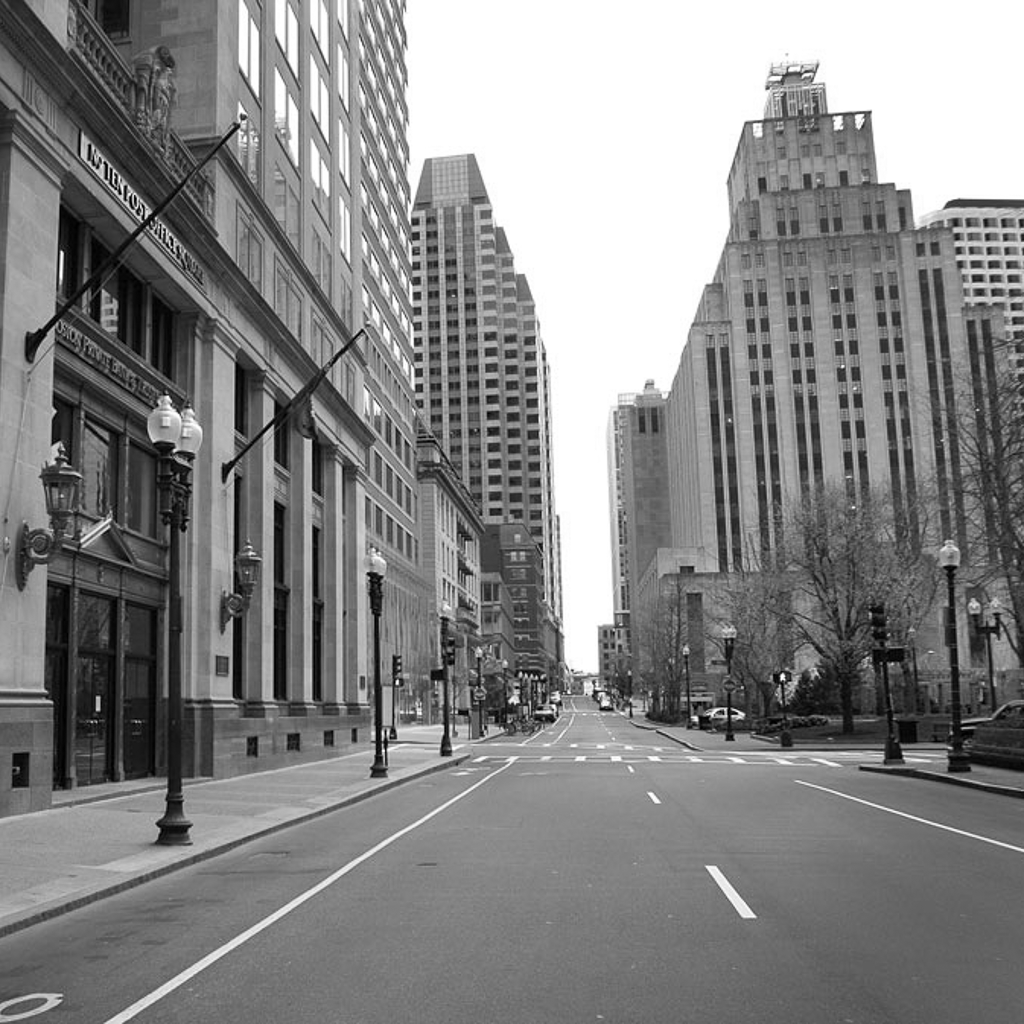
\includegraphics[width=1.4cm]{images/introduction/street1024.png}};
        \node[inner sep=0pt, anchor=west] (whitehead) at ($(cmonitor) + (1.7,0)$)
            {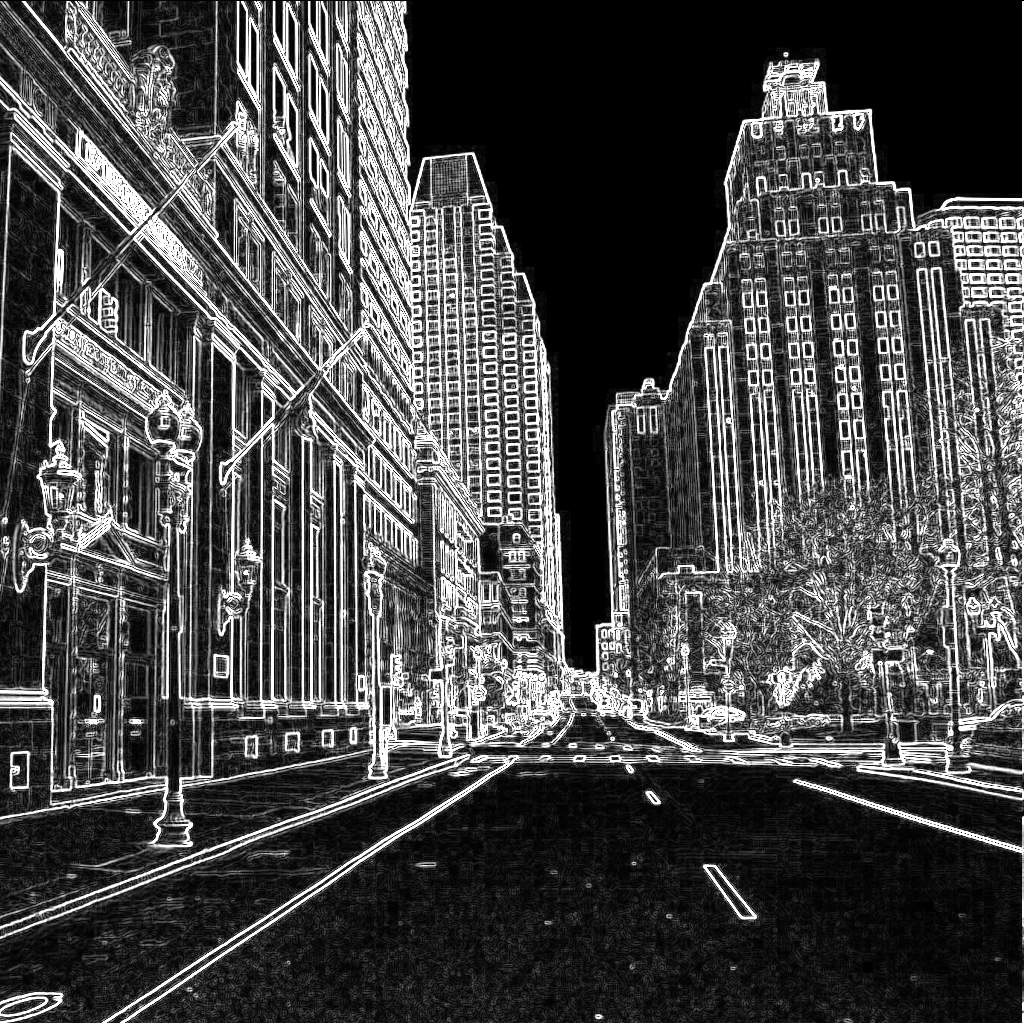
\includegraphics[width=1.4cm]{images/introduction/c_street1024.png}};

        \node[] (eth) at ($(cmonitor) + (4.5, 1.0)$) {LAN};
        
        \draw[line width = 0.5mm] ($(eth) + (0,-1.0)$) ellipse (0.2cm and 0.5cm);
    \end{pgfonlayer}

    % FPGA box
    \begin{pgfonlayer}{main}
        \node[above = 0.2cm of com, xshift=-1.5cm] (fpga) { FPGA };
    \end{pgfonlayer}
    \begin{pgfonlayer}{foreground}
        \node (f_fpga) [draw=black, fill=gray!20, inner sep=20, fit={(com) (ip) }] {};
    \end{pgfonlayer} 

    
    \path[draw,-{Latex[length=2.5mm]}] ($(mon.0) + (0,0.2)$) -- ($(com.180) + (0,0.2)$) node[near end, above] () {1.} ;
    \path[draw,{Latex[length=2.5mm]}-] ($(mon.0) + (0,-0.2)$) -- ($(com.180) + (0,-0.2)$) node[near end, below] () {4.} ;

    \path[draw,-{Latex[length=2.5mm]}] ($(com.0) + (0,0.2)$) -- ($(ip.180) + (0,0.2)$) node[midway, above] () {2.} ;
    \path[draw,{Latex[length=2.5mm]}-] ($(com.0) + (0,-0.2)$) -- ($(ip.180) + (0,-0.2)$) node[midway, below] () {3.} ;

\end{tikzpicture}
%     \caption{Data Flow}
%     \label{fig:datafl}
% \end{figure}

% Sections with NEW are written new in p6
% What is used to realize...
% NEW Dataflow
The existing communication solution is file transfer oriented and stores
received data in memory. This has worked as a proof of concept but is not
optimal
for high throughput image processing. The communication part is extended with an
acknowledge mechanism that allows retransmission of lost packets and a streaming
interface which enables immediate processing of the image data. Furthermore a
memory management unit is introduced that caches image data to reduce bandwidth
usage.

% NEW Image processing
In the preceeding project a Sobel filter was implemented using Vivado HLS. It
uses a simple convolution matrix for edge detection. This operation was well
suited for the first image processing task and to become acquainted with a high
level synthesis tool. For this thesis a new image processing task is realized: the
local contrast enhancement operation called Wallis filter. The algorithm is
described and thoroughly
tested in C/C++ and then synthesized to HDL by the Xilinx Vivado HLS toolchain.
To improve throughput and compare the results of high level synthesis versus a
low level HDL approach, the same filter is implemented in VHDL.

% NEW Scalability
The main intention behind using Ethernet as communication was that the
processing could be distributed onto multiple FPGA. Methods on scalability are
analyzed and compared.

An Artix7 Evaluation Kit by Xilinx serves as a development and testing platform.
It is equipped with gigabit Ethernet LAN and an FPGA with sufficient logic
elements and memory for both the communication and image processing task.
\\

% NEW What is the result of the project
The result is a complete image processing pipeline that begins on a PC where the
input image is sent via Ethernet to the FPGA where it is processed and sent pack
to the PC. The achieved image throughput is 4.1MB/s primarily limited by the image processing core. The Wallis filter core alone
is capable of processing up to 125 megapixels per second on the input. A
benchmark shows the performance differences between a CPU based and FPGA based
solution. 
Concepts on scalability show how the processing power of FPGAs can be
exploited if multiple FPGAs would work on a network. The total throughput then
increases proportional to the number of FPGAs used in the cluster and multiple
gigabytes per seconds of throughput is possible.
\\

% NEW How the document is built up
This report contains six main parts: Theoretical background, mission,
image processing, dataflow, scalability and verification/benchmark.  The
theoretical background explains
the basics of image processing, FPGA, Ethernet communication and on chip
interfaces. The chapter mission will
cover the starting point and presents the concept. Chapters 
image processing and dataflow cover the actual
implementation process of the image processing and dataflow parts.
Before verifying these components in the verification and benchmark chapter the
scalability is studied.


% ------------------------------------------------------------------------->>> %



%%%%%%%%%%%%%%%%%%%%%%%%%%%%%%%%%%%%%%%%%%%%%%%%%%%%%%%%%%%%%%%%%%%%%%%%%%%%%%%%
% 							P R O J E C T   R E P O R T  					   %
%%%%%%%%%%%%%%%%%%%%%%%%%%%%%%%%%%%%%%%%%%%%%%%%%%%%%%%%%%%%%%%%%%%%%%%%%%%%%%%%
\part*{Project Report}
\label{part:project_report}

% <<< ----------------------------------------------------------------- THEORY %
% =============================================================================
%
%                             Theory
%
% =============================================================================
% -----------------------------------------------------------------------------
\chapter{Theoretical Background} \label{chapt:theoreticalback}
% -----------------------------------------------------------------------------
This chapter provides the theory required for the project. On the one hand, it is about image processing and filtering as well as communication via Ethernet. What kind of image operations are possible and the Wallis filter are explained in the chapter \ref{chapt:theory:imageprocessing}. An overview of the communication via Ethernet is provided in the chapter \ref{chapt:theory:ethernet}.


% =============================================================================
%
%                          Image Processing
%
% =============================================================================
\section{Image Processing} \label{chapt:theory:imageprocessing}
In technical terms, image processing is the processing of image data. This includes image processing, image analysis and the output of image files \cite{image_processing}. Procedures that generate a new image can be distinguished into point operations, neighborhood operations and global operations based on their input data. \\
The second part explains the Wallis filter used in this project.

% -----------------------------------------------------------------------------
\subsection{Operations}
% -----------------------------------------------------------------------------
The types of operations that can be applied to images to transform an input image I(u, v) to an output image I'(u, v) can be divided into three categories, which are explained in the following three sections.

\subsubsection*{Point Operations}
The point operations use the color or intensity information at a given pixel in the image as input, calculates a new intensity value as the result and stores it to the same point in the target image (figure \ref{fig:image_operation}a). Typical applications of point operations are, for example, the correction of contrast and brightness, color correction by rotating the color space or the application of different threshold value methods.

Example for a point operation with $u$ and $v$ being pixel coordinates:
\begin{equation}
    I'(u, v) = f(I(u, v))
    \label{eq:point_operation}
\end{equation}


\subsubsection*{Neighborhood Operations} \label{ch:th:neighborhood}
Neighborhood operations use a certain amount of neighboring pixels as input (figure \ref{fig:image_operation}b).
They calculate the result and stored it at the reference point in the target
image. Neighborhood operations are often used in convolution filters. These
filters can be used, for instance, to implement smoothing filters such as the
Gauss filter. Convolution filters can also be used to detect edges in an image. For example, this is possible with the Sobel filter.

Example to calculate the x-derivative and y-derivative with the Sobel matrix \cite{sobel_matrix}:

\noindent\begin{minipage}{.5\linewidth}
\begin{equation}
    G_{x} = I * \begin{bmatrix}
                -1 & 0 & 1 \\ 
                -2 & 0 & 2 \\ 
                -1 & 0 & 1
                \end{bmatrix}
    \label{eq:neighborhood_operation}
\end{equation}

\end{minipage}%
\begin{minipage}{.5\linewidth}

\begin{equation}
    G_{y} = I * \begin{bmatrix}
                -1 & -2 & -1 \\ 
                0 & 0 & 0 \\ 
                1 & 2 & 1
                \end{bmatrix}
    \label{eq:neighborhood_operation}
\end{equation} 

\end{minipage}\\


\textbf{Border Handling:}
With the application of filters, the so-called border handling problem occurs in every image (see figure \ref{fig:image_handling}). Because the filter protrudes beyond the original image.

There are several possible solutions to this issue:
\begin{itemize}
\item The border pixels are not considered. In the example image, the original image 
is two pixels smaller in height and width than the original image. \ref{fig:image_handling}
\item If the filter exceeds the original image, the filter coefficients
at the outside of the image are set to zero
\item The pixels required outside the image are extrapolated according to the closest pixels
\item The image is continued periodically
\end{itemize}
    
\begin{figure}[b!]
    \centering
    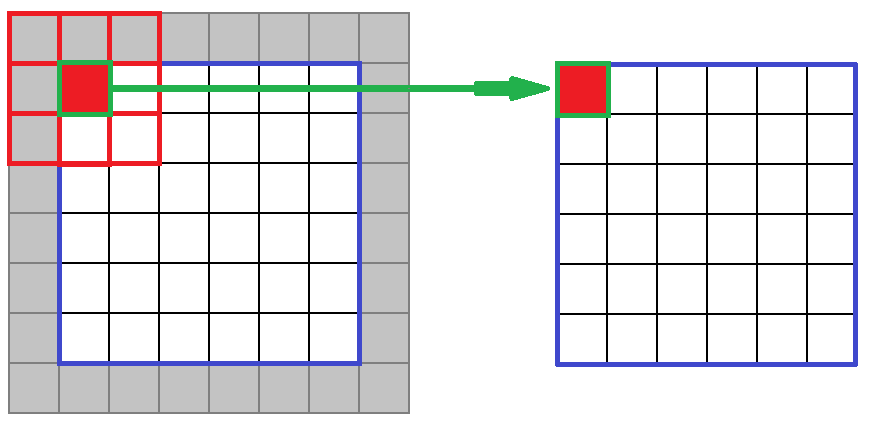
\includegraphics[width=0.6\textwidth]{images/theory/border_handling.png}
    \caption{Border problem with filter operations \cite{border_handling}}
    \label{fig:image_handling}
\end{figure}


\subsubsection*{Global Operations}
Image analysis often employs global image operations that uses the entire image as input data (figure \ref{fig:image_operation}c). It is often about finding regions or recognizing geometrical objects. A typical representative of this is the Hough transform and the Fourier transform.

\begin{figure}[tb!]
    \centering
    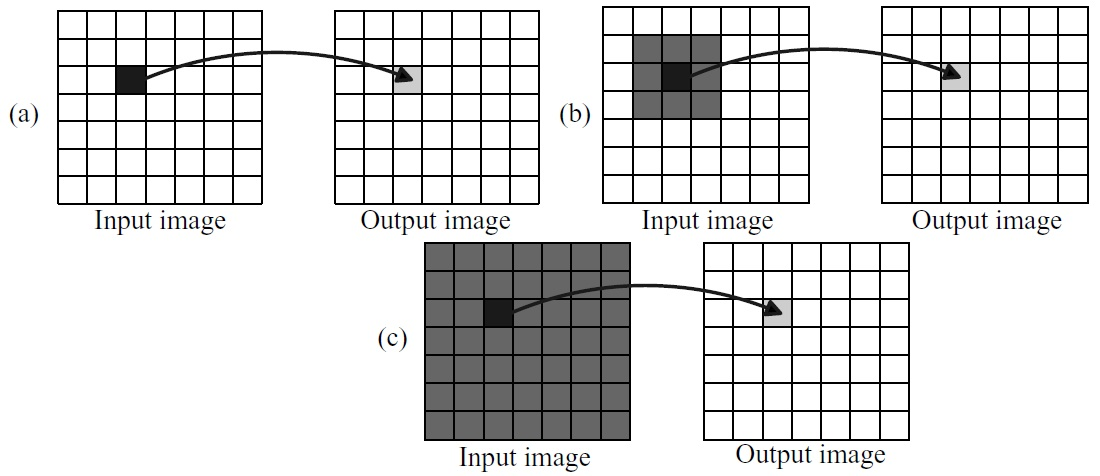
\includegraphics[width=\textwidth]{images/theory/image_operations.jpg}
    \caption{(a) point, (b) neighborhood and (c) global image processing
    operations \cite{image_operation}}
    \label{fig:image_operation}
\end{figure}

% -----------------------------------------------------------------------------
\subsection{Wallis Filter}\label{ch:th_wallis_filter}
% -----------------------------------------------------------------------------
The main goal of the Wallis filter is to adjust the mean and variance of an image and to map it into a given mean and variance to the destination image. This is mainly used for local contrast enhancement in both low and high level regions. It also achieves similair brightness levels in the image.
The Wallis filter equation is \cite{wallis_filter}:
\begin{equation}
    I'(x,y) = \frac{( I(x,y) - \mu_{n})\cdot c \cdot \sigma_{g}^{2}}{c \cdot \sigma_{n}^{2} + (1 - c) \cdot \sigma_{g}^{2}} + b \cdot \mu_{g} + (1 - b) \cdot \mu_{n}
    \label{eq:wallis_filter}
\end{equation} 

\begin{tabular}{rl}
    $I(x,y)         =$ & gray value pixel of the original image \\
    $I'(x,y)        =$ & calculated pixel with the Wallis algorithm \\
    $\mu_{n}        =$ & mean from the neighborhood of the pixel I(x,y) \\
    $\sigma_{n}^{2} =$ & variance from the neighborhood of the pixel I(x,y) \\
    $\mu_{g}        =$ & mean from the destination image \\
    $\sigma_{g}^{2} =$ & variance from the destination image \\
    $b              =$ & brightness factor \\
    $c              =$ & contrast factor \\
\end{tabular} \\

The two facotrs b and c can have the range from 0 to 1. The larger b is selected, the closer it converges to the mean of the desired image $\mu_{g}$. The smaller b is selected, the more it converges to the neighborhood mean $\mu_{n}$.
The bigger the factor c is chosen, the larger is the range of the variance constant $\sigma_{g}^{2}$ \cite{wallis_filter}. \\
The size of the neighborhood depends on the sensor resolution of the camera. The size can be selected from a minimum of 11 to 41 \cite{zeng_2018}. Through the neighborhood operation the smoothing operator is introduced. This means it reduces noise and improves the singal to noise ratio of the image. This in turn enhances image quality \cite{wallis_filter}.


% =============================================================================
%
%                             Ethernet
%
% =============================================================================
\section{Ethernet Communication} \label{chapt:theory:ethernet}
Exchanging data between two devices can be done using different approaches. The
following section contains an overview of the communication standards used in
local area networks (LAN).


\subsection{Open Systems Interconnection (OSI) Model}
Such a telecommunication system can be characterized by the Open Systems 
Interconnection Model. The OSI model is a stack of seven abstraction layers 
grouped into two groups: The host layers and the media layers (see figure \ref{fig:osi}). 
Each layer serves the layer above it and is served with data from the layer
beneath it. In the following chapters the OSI reference model is used to
characterize the Ethernet standard.

\begin{figure}[tb!]
    \centering
    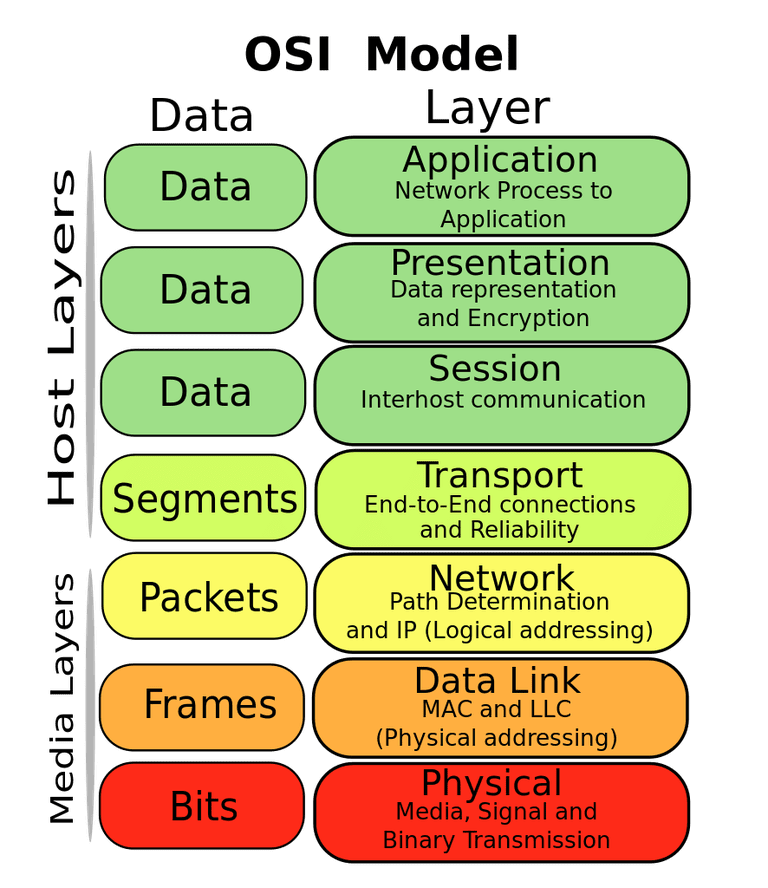
\includegraphics[width=0.5\textwidth]{images/theory/osi.png}
    \caption{OSI Model \cite{osi}}
    \label{fig:osi}
\end{figure}


\subsection{Physical} \label{chapt:theory:physical}
The first layer of the OSI model is the physical layer. It defines the electrical and physical specification of the connection. In the case of local
area networks the connection medium is usually copper. The circuitry required to implement the physical layer is done by the PHY-Chip. This integrated circuit provides digital access through a media independent interface (MII) to the analog physical data link.


\subsection{Data Link} 
The data served from the physical layer is then passed to the data link layer.
Its main purpose is to ensure a reliable transfer of data frames between two
nodes connected by a physical layer. It may also provide means to detect errors
that may occur in the physical layer. Ethernet is the protocol used in the data
layer of local area networks and the layer is split into two sublayers, the logical link control (LLC) and the medium access control (MAC). The LLC provides means to allow multiple network protocols (OSI layer three) to be multiplexed onto the same medium. The MAC encapsulates higher level frames into frames appropriate to be transmitted by the physical layer.
\\

Figure \ref{fig:eth} shows an Ethernet frame. The first seven bytes consist of a fixed preamble. It allows devices on the network to easily synchronize their 
clocks for bit-level synchronization. It is followed by the start frame delimiter (SFD) that marks the beginning of a frame. Sender and receiver MAC addresses ensure that the packet is received by the corresponding host and that it can reply to the sender. The type field indicates the protocol used on the next layer (network layer). After the data payload a frame check sequence in form of a CRC (cyclic redundancy check) is sent to provide error detection. The maximum data payload size is limited to 1500 bytes.
\\

\begin{figure}[tb!]
    \centering
    \begin{adjustbox}{max width=\textwidth}
        \begin{tikzpicture}[
    rounded corners=0mm,
]
    %nodes
    \node[draw, minimum height=1.0cm] (pre) {Preamble};
    \node[draw, minimum height=1.0cm, right = 0cm of pre] (sfd) {SFD};
    \node[draw, minimum height=1.0cm, right = 0cm of sfd] (dst) {Destination MAC Adr.};
    \node[draw, minimum height=1.0cm, right = 0cm of dst] (src) {Source MAC Adr.};
    \node[draw, align = center, text width=1cm, minimum height=1.0cm, right = 0cm of src] (tp) {Type\\Field};
    \node[draw, minimum height=1.0cm, right = 0cm of tp] (dat) {Data (46 - 1500 Bytes)};
    \node[draw, minimum height=1.0cm, right = 0cm of dat] (pad) {PAD};
    \node[draw, minimum height=1.0cm, right = 0cm of pad] (crc) {CRC};

    \path[draw,-] ($(dst.180) + (0,0)$) -- ++(0,1.2) ;
    \path[draw,-] ($(crc.0) + (0,0)$) -- ++(0,1.2) ;
    \path[draw,{Latex[length=2.5mm]}-{Latex[length=2.5mm]}] ($(dst.180) + (0,1.0)$) -- ($(crc.0) + (0,1.0)$) node [midway, above] () {Basic MAC Frame} ;
\end{tikzpicture}
    \end{adjustbox}
    \caption{Ethernet Frame}
    \label{fig:eth}
\end{figure}
The medium access controller is implemented in hardware to ensure that every bit is received and stored. The transmit and receive data is commonly stored in
FiFo (first in first out) buffers. This way the next layer in the OSI model is
not required to have low latency capability.


\subsection{Network} 
The data link layer provides means to send frames across nodes in the same
network. As soon as the destination node is in another network, a network layer
is required. Using logical device addresses, network packets can be routed
across different networks and on different media. This allows data to be sent
over long distances.
\\

The most commonly used network layer is the Internet Protocol version 4 (IPv4).
It consists of a 20 byte sized header that contains destination and source IP
addresses, total length, checksum and other fields. The protocol field indicates what layer four protocol is used. Figure \ref{fig:ip} shows a complete IPv4 header.

\begin{figure}[tb!]
    \centering
    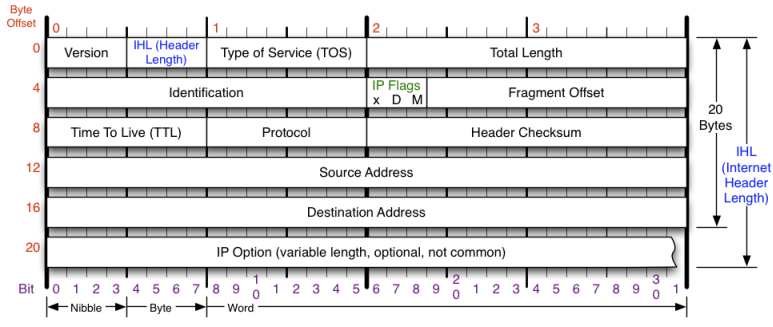
\includegraphics[width=\textwidth]{images/theory/ip.png}
    \caption{IPv4 header \cite{ip}}
    \label{fig:ip}
\end{figure}
\begin{figure}[tb!]
    \centering
    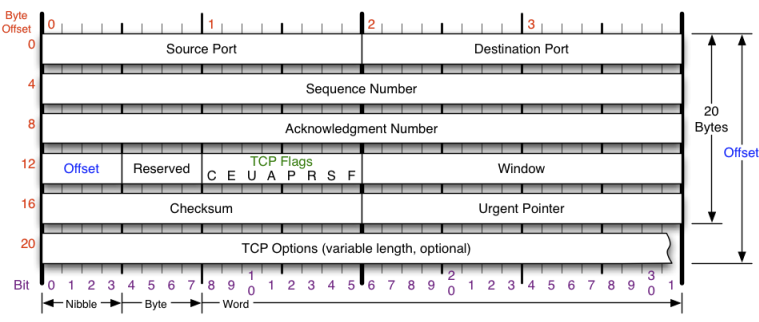
\includegraphics[width=\textwidth]{images/theory/tcp.png}
    \caption{TCP Header \cite{tcpudp}}
    \label{fig:tcp}
\end{figure}
\begin{figure}[tb!]
    \centering
    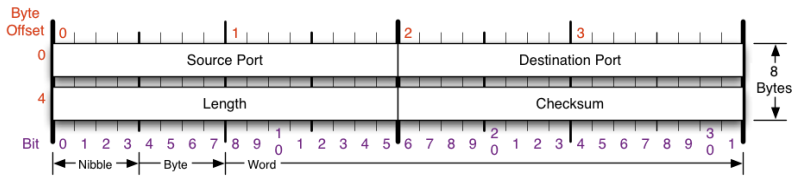
\includegraphics[width=\textwidth]{images/theory/udp.png}
    \caption{UDP Header \cite{tcpudp}}
    \label{fig:udp}
\end{figure}


\subsection{Transport} 
The transport layer is the first layer in the OSI model that is not required by
the network. Its main purpose is to control the communication of different
applications on two hosts. Therefore a port number is required to distinguish
between the different applications utilizing the same network connection. The
transport layer may also provide segmentation of the data, guarantee of delivery and flow control to avoid network jam.
\\

The two most used transport layer protocols are the Transmission Control
Protocol (TCP) and the User Datagram Protocol (UDP). Table \ref{tab:tcpudp}
shows the main differences between these two protocols. The most important
aspect is the protocol connection setup. While UDP is connection less (data is
sent without setup), TCP establishes a connection between host and client
prior to data transmission. This ensures a reliable data delivery hence all
messages are acknowledged. UDP has its benefits in lower overhead and for that
reason has slightly higher transmission speed but the protocol does not
guarantee that the message has been received by the client.

\begin{table}[h]
    \centering
    \begin{tabular}{ l  c  c }
        \toprule
         & \textbf{TCP} & \textbf{UDP} \\
        \midrule
        Connection oriented & Yes & No \\
        Header size & 20 Byte & 8 Byte \\
        Reliable transmission & Yes & No \\
        Acknowledge & Yes & No \\
        Segmentation & Yes & No \\
        Best for & reliable transfer & fast transfer  \\
        \bottomrule
    \end{tabular}
    \caption{TCP vs. UDP}
    \label{tab:tcpudp}
\end{table}

\section{Vivado HLS} \label{ch:th:hls}
Vivado HLS is a development environment that synthesizes C/C++ code in VHDL. The C/C++ language is intended for sequential programming where the VHDL language describes the hardware. This chapter deals with the design flow (\ref{ch:design_flow})of Vivado HLS. The directives (\ref{ch:directives}) that are for the compiler to synthesize the C/C++ code in VHDL and finally arbritary data types (\ref{ch:ap}). Which can be used in the Vivado HLS for C/C++ code.

\subsection{Design Flow} \label{ch:design_flow}
In Vivado HLS it is possible to translate the C/C++ code into VHDL and generate an IP core for Vivado HLx. To ensure that the algorithm is correct, it can be validated in various steps. These steps are the design flow of Vivado HLS and are shown in figure \ref{fig:hls_design_flow}.
First of all, the C/C++ algorithm can be tested in a simulation. This requires a testbench in addition to the C/C++ algorithm. As soon as the algorithm works satisfyingly the design can be run through synthesis and generating a RTL design in VHDL. VHDL design can be verified in an RTL simulation. The RTL simulation must match the C/C++ simulation. If this is the case, an IP core can be generated from the VHDL code and used in the Vivado HLx \cite{vivado_hls}.

\begin{figure}[tb!]
    \centering
    % \tikzsetnextfilename{system-overview}
\begin{tikzpicture}[
    rounded corners=0mm,
]
    %coordinates
    \coordinate (orig)      at (0,0);
    \coordinate (test)      at (-3,0);
    \coordinate (alg)       at (3,0);
    \coordinate (c_sim)     at (0,-1);
    \coordinate (c_synth)   at (0,-2);
    \coordinate (VHDL)      at (0,-3);
    \coordinate (rtl_sim)   at (0,-4);
    \coordinate (ip)        at (0,-5);
    \coordinate (hlx)       at (0,-6);

    %nodes
    \node[draw, fill=white, minimum width=4cm, minimum height=0.6cm, anchor=south, text width=3.8cm, align=center, rounded corners=3mm] (A) at (test) {C/C++ Testbench};
    \node[draw, fill=white, minimum width=4cm, minimum height=0.6cm, anchor=south, text width=3.8cm, align=center, rounded corners=3mm] (B) at (alg) {C/C++ Algorithm};
    \node[draw, fill=white, minimum width=4cm, minimum height=0.6cm, anchor=south, text width=3.8cm, align=center] (C) at (c_sim) {C/C++ Simulation};
    \node[draw, fill=white, minimum width=4cm, minimum height=0.6cm, anchor=south, text width=3.8cm, align=center] (D) at (c_synth) {C/C++ Synthesis};
    \node[draw, fill=white, minimum width=4cm, minimum height=0.6cm, anchor=south, text width=3.8cm, align=center, rounded corners=3mm] (E) at (VHDL) {VHDL};
    \node[draw, fill=white, minimum width=4cm, minimum height=0.6cm, anchor=south, text width=3.8cm, align=center] (F) at (rtl_sim) {RTL Simulation};
    \node[draw, fill=white, minimum width=4cm, minimum height=0.6cm, anchor=south, text width=3.8cm, align=center] (G) at (ip) {Package IP};
    \node[draw, fill=white, minimum width=4cm, minimum height=0.6cm, anchor=south, text width=3.8cm, align=center] (H) at (hlx) {Vivado HLx};

    %path
    \path [draw,-] (A) -- (B);
    \path[draw,-{Latex[length=2.5mm]}] (A) -| (C);
    \path[draw,-{Latex[length=2.5mm]}] (C.east) -- ++(3.5,0) |- (B.east);
    \path[draw,-{Latex[length=2.5mm]}] (C) -- (D);
    \path[draw,-{Latex[length=2.5mm]}] (D) -- (E);
    \path[draw,-{Latex[length=2.5mm]}] (E) -- (F);
    \path[draw,-{Latex[length=2.5mm]}] (E.west) -- ++(-0.5,0) |- (G.west);
    \path[draw,-{Latex[length=2.5mm]}] (F.east) -- ++(3.5,0) |- (B.east);
    \path[draw,-{Latex[length=2.5mm]}] (G) -- (H);


\end{tikzpicture}
    \caption{Vivado HLS design flow}
    \label{fig:hls_design_flow}
\end{figure}

\subsection{Directives} \label{ch:directives}
If the FPGA is programmed using C/C++ language, there is no way to get around the directives. Directives are instructions to the compiler on how it should synthesize and optimize the code. Latency, throughput or area can be optimized \cite{pragma}. The following three chapters explain some important directives to reduce the latency and increase the throughput. \\
Directives are also called pragmas and can be written directly into the C/C++ code or added as directives in a separate tcl-file.

\todo[inline]{Bilder von Interfce, Array Partition und Pipeline / Unroll anpassen!}

\subsubsection*{Interface}
The directive \texttt{interface} specifies the input and output ports of the IP core. Different interfaces can be implemented in the IP core as input and output ports. Among others, these are control interfaces or interfaces for data. \\
The IP core can be controlled with the control interfaces. With this signal it can be started or stopped for example or send a handshake if the IP core has the operation finished. \\
AXI4 interfaces can also be added directly to the IP core by directives. The AX4-Lite, AXI4-Master or AXI4-Stream interface can be connected. \\
Among other things, memory elements can also be connected directly to the IP core. These are block RAM or FIFOs that can be used to read and process the data with the IP core. These can also be used to store output data of the IP core \cite{pragma}. \\
The figure \ref{fig:p_interface} shows how the pragma \texttt{interface} is configured. First, the interface can be specified and whether it is an input or an output. Finally, the variable to which the pragma is to be applied.

\begin{figure}[tb!]
    \centering
    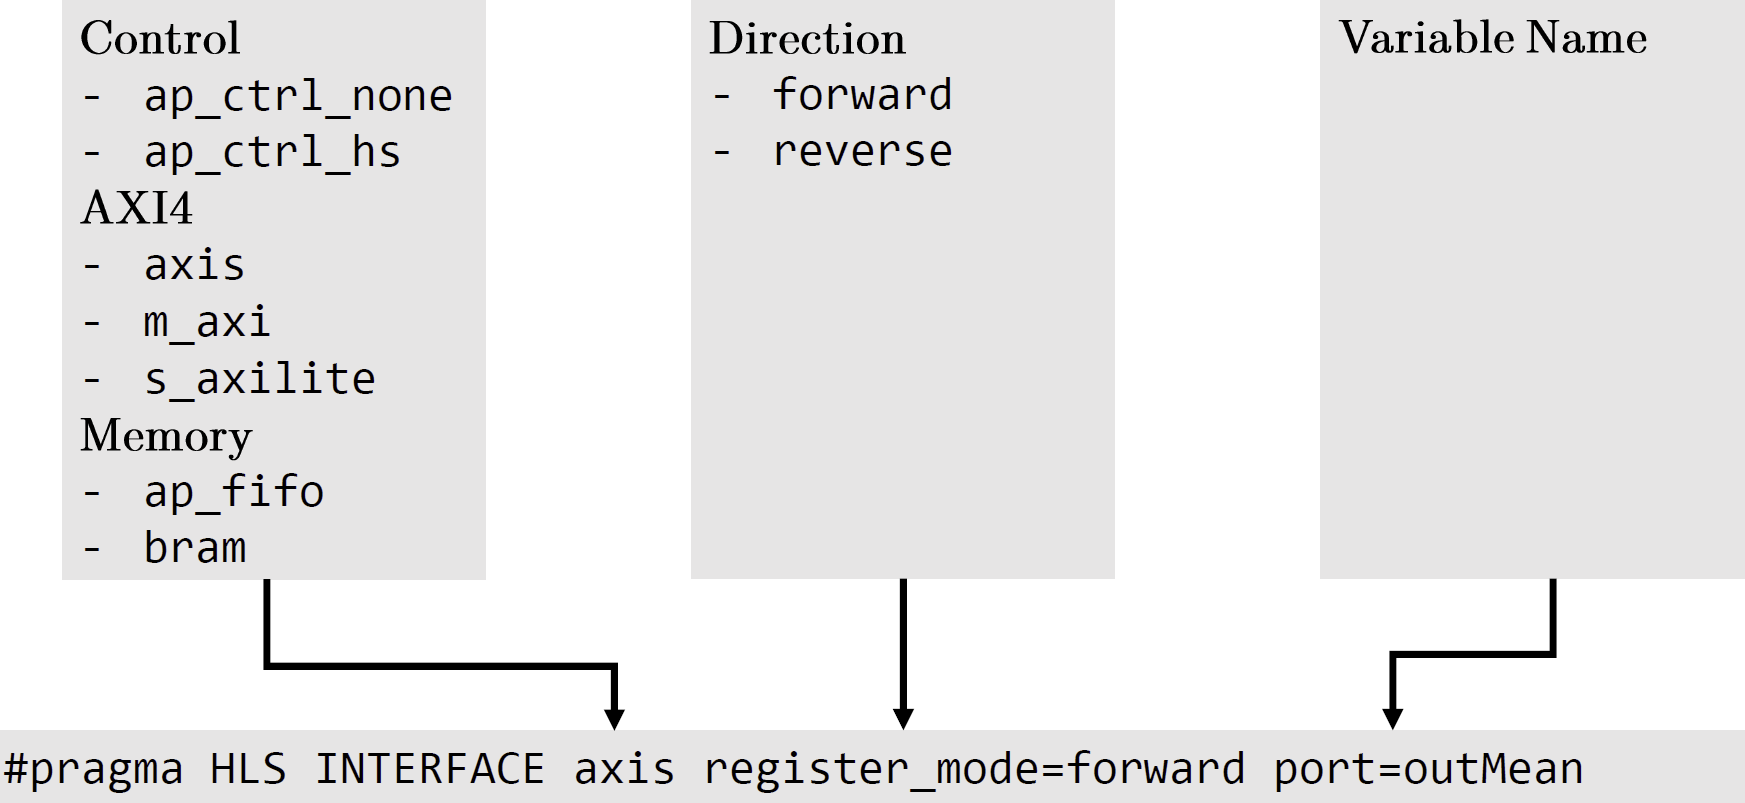
\includegraphics[width=\textwidth]{images/theory/interface.png}
    \caption{Pragma: interface}
    \label{fig:p_interface}
\end{figure}

\subsubsection*{Array Partition}
The \texttt{array\_partition} directive splits an array into several smaller elements. This means that in RTL synthesis several smaller memories or registers are used from a larger memory. However, this increases the throughput in the design but also the read and write ports for the storage. \\
The figure \ref{fig:p_array_partition} shows the three different methods of partitioning an array.

\begin{description}
\item[Block]\hfill \\
The whole array is split into several arrays of the same size. The elements are stored in the same order as in the array. The array is simply cropped apart.
\item[Cyclic]\hfill \\ 
The array is split into equal parts like \texttt{block}, but the storage order is different. As can be seen, each following element is stored in a different memory. 
\item[Complete]\hfill \\ 
This argument splits the complete array into individual elements.
\end{description}


\begin{figure}[tb!]
    \centering
    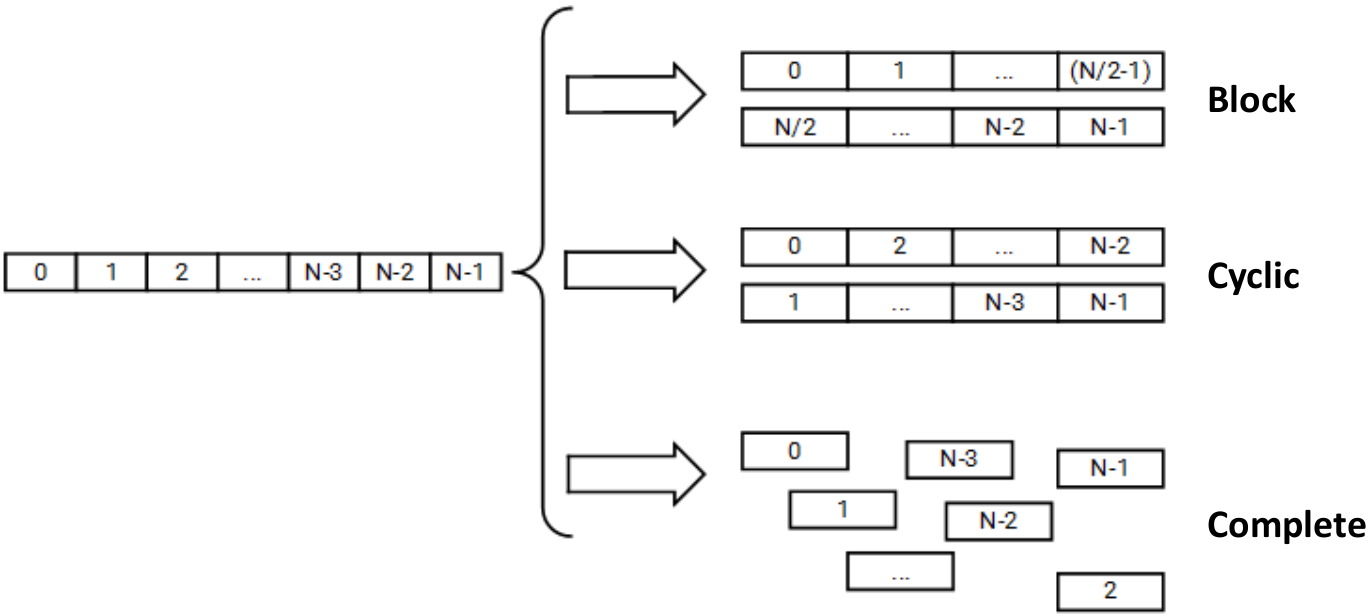
\includegraphics[width=\textwidth]{images/theory/array_partition.png}
    \caption{Pragma: array\_partition}
    \label{fig:p_array_partition}
\end{figure}

\subsubsection*{Pipeline / Unroll}
In Vivado HLS the FPGA is described with C/C++ language. Among others, it is also possible to program for loops. These are still processed sequentially by the RTL synthesis, as can be seen in the figure \ref{fig:p_pipeline_unroll} with 9 clock cycles. The directive can improve the performance of the for loop. Two directives are available to increase the throughput of a for loop. These are \texttt{pipeline} and \texttt{unroll}.

\begin{description}
\item[Pipeline]\hfill \\
This directive allows a for loop to be parallelized. This increases the throughput and the area. Now that more operations are happening in a clock.
Pipeline is used if not all data for processing is available in the for loop. The figure \ref{fig:p_pipeline_unroll} shows that the read access leads to a latency of one clock cycle and the throughput could be increased.
\item[Unroll]\hfill \\ 
This directive allows the for loop to be fully parallelized. This is only possible if all the data that is required in the for loop is available. The figure \ref{fig:p_pipeline_unroll} shows that the entire for loop is now processed in one cycle. This again leads to an increase in throughput and the area in relation to directive \texttt{pipeline}.
\end{description}

With nested for loops, note that if pipeline is applied to the top loop, the inner for loops are automatically unrolled. \\
You can also apply both directives in combination in a for loop. Since the unroll directive can specify a factor that unrolls the loop.

\begin{figure}[tb!]
    \centering
    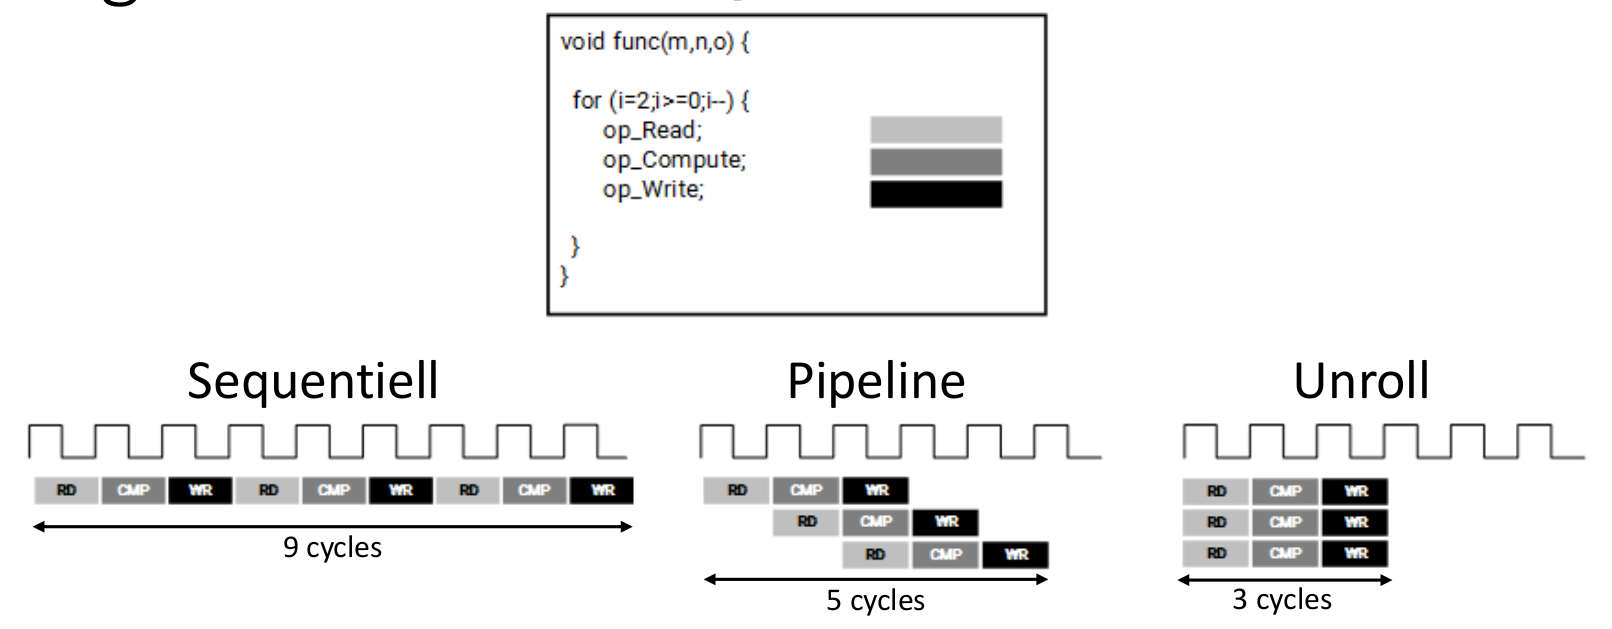
\includegraphics[width=\textwidth]{images/theory/pipeline_unroll.png}
    \caption{Pragma: pipeline / unroll}
    \label{fig:p_pipeline_unroll}
\end{figure}

\subsection{Arbitrary Precision} \label{ch:ap}
Resources are limited in the FPGA. Therefore it is often a big waste of resources when calculating with too large data types or even floating point in the FPGA \cite{floating}. Viviado HLS supports arbitrary precision data types using C/C++ code. With this it is possible to counteract the problem of large data types and floating point. \\

\textbf{Arbitrary Precision Integer:}
Arbitrary Precision Integers are data types where it is possible to define any bit width. This has the advantage that resources can be reduced. Because it is not necessary to select the data types provided in C/C++ (8, 16, 32 bit or char, short, int etc.) \\
To use these data types only the header file \texttt{ap\_int.h} must be included. The following example shows how a 11 bit signed integer and a 5 bit unsigned integer be defined \cite{ug902}.

\begin{minipage}{\textwidth}
\begin{lstlisting}[style=CStyle]
ap_int<11> var1;
ap_uint<5> var2;
\end{lstlisting}
\end{minipage} \\

\textbf{Arbitrary Precision Fixed-Point:}
Floating Point can be used on the FPGA, but this usually requires a lot of resources. Viviado HLS has a library for Arbitrary Precision Fixed Point data types, which can be used to calculate sufficiently accurate. With these fixed point data types many resources can be saved. \\
For this purpose there is the library \texttt{ap\_fixed.h} and must be included. The data types are defined so that the first number represents the whole data type width and the second number represents the above number of the binary point. The following example shows an unsigned 11 bit varibale with 3 bits representing the integer value and 8 bits representing the fractional value \cite{ug902}. 

\begin{minipage}{\textwidth}
\begin{lstlisting}[style=CStyle]
ap_ufixed<11,3> fp_var;
\end{lstlisting}
\end{minipage}

% =============================================================================
%
%                          AXI4 Interfaces
%
% =============================================================================
\section{AXI4 Interfaces} \label{chapt:theory:axi4interfaces}
Advanced eXtensible Interface or AXI is part of the Advanced Microcontroller Bus
Architecture (AMBA\textregistered) introduced by ARM\textregistered \cite{axispecs}. 
It is intended for the interconnection of functional blocks inside a System on
Chip or FPGA. IP cores offered by Xilinx implement these interfaces. Two types
of AXI interfaces are destinguished: Memory mapped and stream. Memory mapped
interfaces intend the bidirectional access to data stored in registers while
streaming interfaces offer a unidirectional dataflow \cite{axistreamspecs}.

\subsection{AXI4} \label{chapt:theory:axi4}
The AXI4 interface is a memory mapped interface and consists of five transaction
channels as shown in table
\ref{tab:axi4transchan}. 

\begin{table}[h]
    \centering
    \begin{tabular}{ l  l}
        \toprule
        Transaction Channel & Use \\
        \midrule
        Write address channel & Generate write requests to slave \\
        Write data channel & Write data to be sent to the slave \\
        Write response channel & Write response from slave to master \\
        Read address channel & Generate read requests to slave \\
        Read data channel & Read data from slave to master \\
        \bottomrule
    \end{tabular}
    \caption{AXI4 transaction channels}
    \label{tab:axi4transchan}
\end{table}

Each channel has its own handshake signals. Handshake signals are used to
indicate that the sender has valid data and the receiver is ready to accept
data. Figure \ref{fig:axihandshake} shows the handshake signals. The VALID
signal is set active if the sender has driven the INFORMATION lines with valid
data. The receiver indicates with a READY impulse that it has read the
information. 

\begin{figure}[h!]
    \centering
    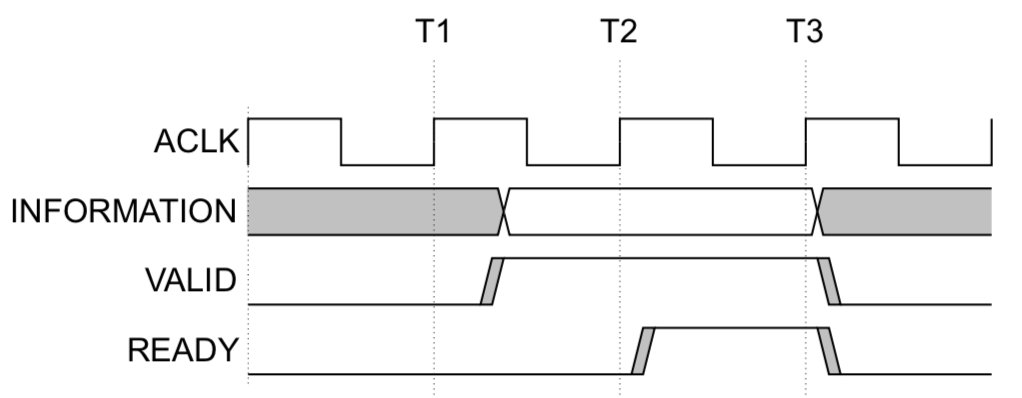
\includegraphics[width=0.6\textwidth]{images/theory/axi4handshake.png}
    \caption{VALID before READY handshake \cite{axispecs}}
    \label{fig:axihandshake}
\end{figure}

A AXI4 write transaction could run as followed:
\begin{itemize}
    \item Master sends address and burst size through write address channel
    \item Master sends data through write data channel
    \item Slave responds with status on write response channel
\end{itemize}

A AXI4 read transaction could run as followed:
\begin{itemize}
    \item Master sends read address and burst size through read address channel
    \item Slave responds with data on read data channel
\end{itemize}

A burst transacion allows to send or receive a range of data with a single write
request while a single beat transaction consists of one write request and one
data word.

\subsection{AXI4-Lite}
AXI4-Lite is a scaled-down version of AXI4. It allows single beat write and
reads but no burst transaction. It therefore requires less signals and is suited
for configuering IP cores and register values. It consists of the same
transaction channels and handshake signals. AXI4 and AXI4-Lite are compatible
and can be converted.

\subsection{AXI4-Stream}
AXI4-Stream is a stream based interfaces. Data is sent in one direction from
master to slave. It is not address based and features only one transaction
channel. There is also no burst size limit. There are four required signals as
shown in table \ref{tab:axi4steramreqsig}.

\begin{table}[h]
    \centering
    \begin{tabular}{ l  l l}
        \toprule
        Signal & Source & Description \\
        \midrule
        \texttt{ACLK} & Master & Rising edge sampled clock signal \\
        \texttt{ARESETn} & Master & Global active low reset signal \\
        \texttt{TVALID} & Master & indicates that the master is driving a valid transfer
        \\
        \texttt{TREADY} & Slave & indicates that the slave can accept a transfer \\
        \texttt{TDATA[(8n-1):0]} & Master & Data payload \\
        \bottomrule
    \end{tabular}
    \caption{AXI4-Stream required signals}
    \label{tab:axi4steramreqsig}
\end{table}

\texttt{TVALID} and \texttt{TREADY} are the handshake signals as described in chapter 
\ref{chapt:theory:axi4} and illustrated in figure \ref{fig:axihandshake}.
AXI4-Stream defines further sideband signals, some of which are described in
table \ref{tab:axi4steramside}.

\begin{table}[h]
    \centering
    \begin{tabular}{ l  l l}
        \toprule
        Signal & Source & Description \\
        \midrule
        \texttt{TLAST} & Master & indicates the boundary of a packet \\
        \texttt{TDEST[(d-1):0]} & Master & provides routing information for the data stream \\
        \texttt{TUSER[(u-1):0]} & Master & user defined sideband information \\
        \bottomrule
    \end{tabular}
    \caption{AXI4-Stream sideband signals}
    \label{tab:axi4steramside}
\end{table}

In this project the \texttt{TLAST} signal is used frequently to indicate for
example the end of a file transfer of the communication core or the last pixel
of an image line.


% ------------------------------------------------------------------------->>> %

% <<< ---------------------------------------------------------------- MISSION %
% ==============================================================================
%
%                             Mission
%
% ==============================================================================
\chapter{Mission} \label{chapt:mission}
With the theoretical background covered the mission of this project can be
addressed.
The following sections will first cover the starting point and the available resources. Different possible solutions will be covered in \ref{chapt:solutions} before presenting the concept in chapter \ref{chapt:mission:concept}. \\

In a world of self driving cars and virtual reality, having a digital copy of
the real world yields several benefits. Cars can be trained in a virtual city
to increase the performance of their algorithms and video games could get more
realistic if the player could walk through the streets of a major city. Gathering this data is one problem and processing the images is another. Pictures have to be converted, analyzed and processed. This requires a great deal of computational power for a task that is repeated several times.

% ==============================================================================
%
%                             Starting Point
%
% ==============================================================================
\section{Starting Point}
The goal of this project is to investigate a dedicated hardware approach to
accelerate intense image processing. To do so, a basic image processing
algorithm such as the Wallis filter is implemented on an FPGA that communicates
over a network with a host computer. The image processing task should later be
distributed onto multiple FPGAs to accelerate the processing even more 
\cite{nomokoReqs}. Before listing possible solutions the available resources and
boundary conditions need to be analyzed.

\subsection{FPGA Board} \label{chapt:mission:fpgaboard}
\begin{figure}[tb!]
    \centering
    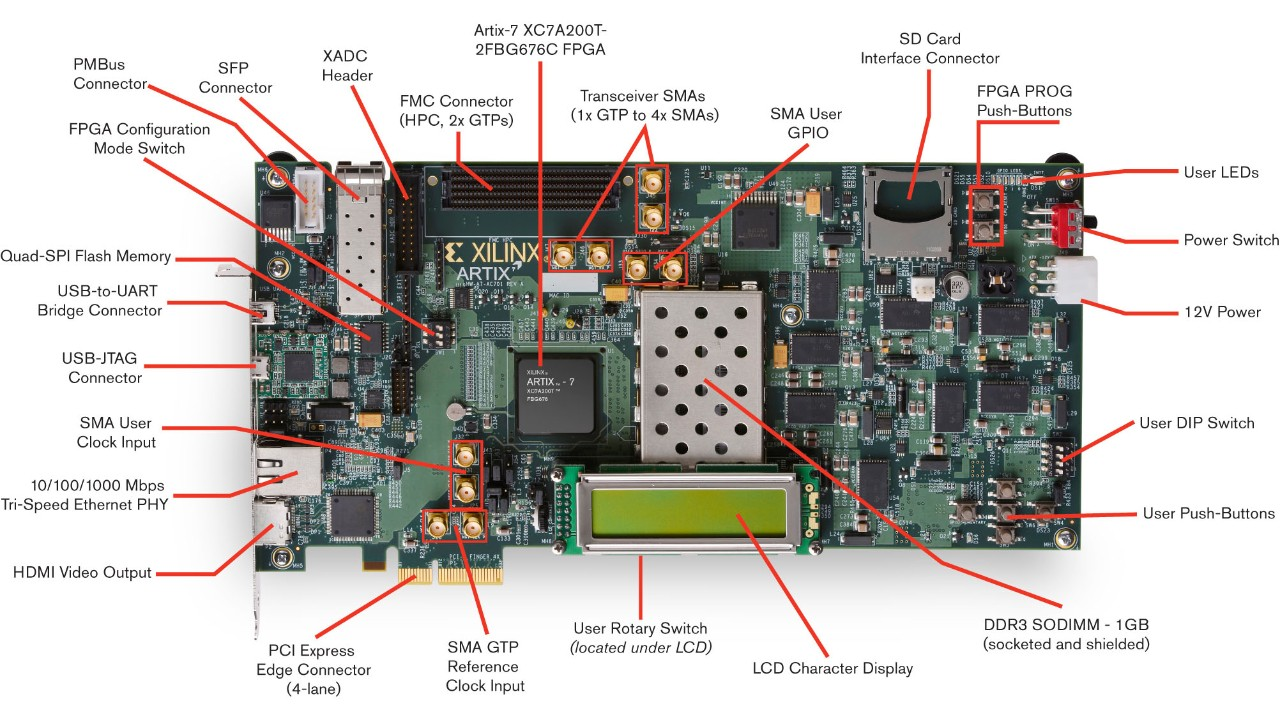
\includegraphics[width=\textwidth]{images/mission/ac701.png}
    \caption{Xilinx AC701 Evaluation Kit \cite{image_ac701}}
    \label{fig:ac701}
\end{figure}

The Xilinx AC701 Evaluation Kit is used as development platform. It features an
Artix-7 FPGA and several useful on-board peripherals. The JTAG interface is used
for configuration and debugging of the FPGA. To connect the platform to the
network, a Gigabit Ethernet PHY handles the first layer of the OSI model in
hardware (see chapter \ref{chapt:theory:physical}). Storing data is possible in the DDR3 memory
module. Table \ref{tab:ac701} shows a summary of the important peripherals on
the AC701 board.
\\
\begin{table}[b!]
    \centering
    \begin{tabular}{l l}
        \toprule
        Part & Description \\
        \midrule
        FPGA & XC7A200T-2FBG676C \\
        JTAG & Onboard JTAG configuration circuitry to enable configuration over USB \\
        Memory & DDR3 SODIMM 1GB up to 533MHz / 1066Mbps \\
        Ethernet & 10/100/1000 Mbps Ethernet (RGMII) \\
        \bottomrule
    \end{tabular}
    \caption{Xilinx AC701 key board features \cite{xilinx_ac701}}
    \label{tab:ac701}
\end{table}

The XC7A200T FPGA is part of the Artix-7 family. It is optimized for high logic
throughput at low costs. Important for this project is the number of logic cells
and the amount of on-chip memory. With more logic cells available, data can be
processed parallel and the throughput increases. Processing more data at the
same time also requires the data to be stored. Therefore on-chip memory, also
called block memory, is used to have fast access to the data. Table 
\ref{tab:XC7A200T} lists the relevant numbers of resources.

\begin{table}[tb!]
    \centering
    \begin{tabular}{l l}
        \toprule
         & XC7A200T \\
        \midrule
        Logic Cells & 215k \\
        DSP Slices & 740 \\
        Block Memory & 1642 KB \\
        \bottomrule
    \end{tabular}
    \caption{XC7A200T key features \cite{xilinx_ac701}}
    \label{tab:XC7A200T}
\end{table}


\subsection{Communication} \label{chapt:mission:communication} 
In the preceding project \cite{p5report} an Ethernet communcation between PC and
FPGA was established. This included a UDP based protocol that was implemented on
the PC and on the FPGA in form of an IP core. Basic file transfers are working
but many features such as reliable transfer using acknowledge and retransmission
only exist on paper. The work in this project is built
upon the IP core from project 5 while improvements and modifications are made to
the IP core.

\begin{figure}[tb!]
    \centering
    % 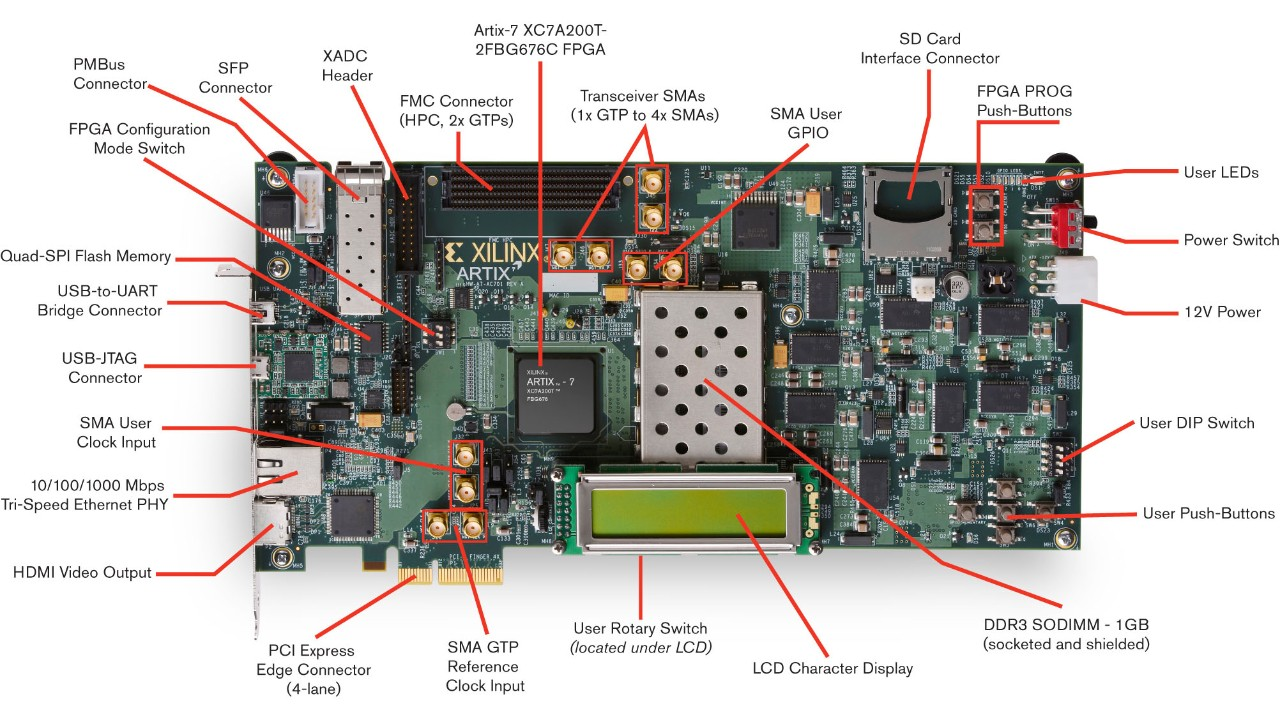
\includegraphics[width=\textwidth]{images/mission/ac701.png}
    \caption{UFT IP core from project 5 \cite{p5report}}
    \label{fig:uftipcorep5}
\end{figure}

\todo[inline]{figure p5 UFT ip core from block design}

\subsection{Image Size}
The customer Nomoko has a camera with a resolution of 1500MPixel (\ref{app:technicial_requirements}). If this is a color image with 24 bit RGB values, the following file size will result:
\begin{equation}
    File Size = Pixel_{tot} * Pixel_{size} = 1500MPixel * 24bit = 36Gbit \cong 4.4GByte
    \label{eq:filesize}
\end{equation}

\subsection{Wallis Filter} \label{chapt:mission:wallis}
The customer Nomoko wants the Wallis filter to be implemented. The Wallis
filter is used for local contrast enhancement. For example, the filter can compensate house shadows in images and get more details from the image. 
The Wallis filter is based on the equation \ref{eq:wallis_filter} as explained in chapter \ref{ch:th_wallis_filter}.


\subsection{Development Environment}
The image processing algorithm is written in Vivado HLS (\ref{app:technicial_requirements}). With Vivado HLS, an IP core for the Vivado HLx can be generated from a C/C++ code. Vivado HLS is useful when programming algorithms and afterwards translating them into hardware description language. \\ 
\\
Communication is implemented with configurable IP blocks provided by Xilinx,
third party providers and custom developed IP cores. Vivado HLS is mainly used
for the dataflow inside the FPGA
(see the technical requirements for more detail in appendix 
\ref{app:technicial_requirements}).

% ==============================================================================
%
%                             Possible Solutions
%
% ==============================================================================
\section{Possible Solutions} \label{chapt:solutions}
With the starting point dissected the possible solutions to the problem can be
stated. They are split into the two parts of image processing and dataflow.

\subsection{Image Processing} \label{chapt:mission:ip}
The Wallis algorithm is based on the neighborhood operation (\ref{ch:th_wallis_filter}). Therefore, the borders of the image must be considered separately (\ref{ch:th:neighborhood}). There are three possible solutions to the border problem:

\begin{itemize}
\item The border pixels are not considered. This means that the destination image will be smaller depending on the size of the neighborhood
\item The pixels required outside the image are extrapolated according to the closest pixels
\item The image is continued periodically
\end{itemize}

\subsection{Dataflow} \label{chapt:mission:dataflow}
As described in \ref{ch:th_wallis_filter} the Wallis filter requires a
neighborhood of pixels to do its calculations. Therefore the data comming from
the communication part must be buffered and fed to the Wallis filter in a given
order. Further details are described in chapter \ref{chapt:dataflow}. Following
realisations may be considered for the control of the dataflow:\\

\textbf{Data preparation on PC:} The image data is prepared on the PC and sent
in the right order. This method is simple to realise and requires no
additional FPGA ressources. On the other hand, data may be sent more than once
which results in a decrease of throughput.\\

\textbf{Soft microprocessor core:} Image data is sent to the FPGA and stored in
FPGA memory. A microcontroller implemented in FPGA logic then dissects the data
and feeds it to the Wallis filter in the right order. Hence the data is buffered
the Ethernet throughtput can reach its maximum. The downside to this
solution
is that such a soft microprocessor core may take more FPGA ressources than a
dedicated approach.\\

\textbf{Controller IP core:} An IP core is developed that handles the specific
task of managing the dataflow between the communication and Wallis cores. This
approach takes little FPGA ressources but involves more time to develop.

\subsection{Scalability} \label{chapt:mission:scalability}
Appendix \ref{app:technicial_requirements} lists two possible solutions to scale
the image processing inside the FPGA. 
\begin{itemize}
    \item Store the image in block memory and distribute it to the image
    processing's local memory for processing
    \item Data is streamed from the communication part directly to the different
    image processing cores
\end{itemize}

% ==============================================================================
%
%                             Concept
%
% ==============================================================================
\clearpage
\section{Concept} \label{chapt:mission:concept}
Now that the possible solutions for dataflow, image processing and scalability
have been discussed, the way of proceeding can be concluded.\\


\textbf{Image processing}
    \begin{itemize}
        \item The border pixels are not considered for simplicity. The destination image will be smaller than the source image.
        \item The image is sent in several pieces to the FPGA since 4.4GB 
        (see equation \ref{eq:filesize}) do not have space on the FPGA (see chapter \ref{chapt:mission:fpgaboard}).
    \end{itemize}

\textbf{Dataflow}
    \begin{itemize}
        \item The communication is extended with acknowledge and retransmission.
        \item A controller IP core is realized to handle the dataflow between
        communication and Wallis filter.
    \end{itemize}

\textbf{Scalability}
    \begin{itemize}
        \item Use stream interfaces on the image processing and dataflow parts
        to enable stream based scalability
        \item Assess the inside and across FPGA scalability in theory
    \end{itemize}


Figure \ref{fig:blockdiagram} shows the conceptual block diagram. Image data is
sent from the PC to the FPGA over Ethernet. The communication block handles the
file transfer and stores the image data in FPGA block memory. A controller core
then feeds the data in the right order to the Wallis filter and stores the
results again in block memory. The controller sends a command to the
communication cores which then starts sending the processed image data back to
the PC.

\begin{figure}[b!]
    \centering
    % \tikzsetnextfilename{system-overview}
\begin{tikzpicture}[
    rounded corners=0mm,
]
    %coordinates
    \coordinate (corig)      at (0,0);
    \coordinate (cmonitor)   at (0,0);
    \coordinate (ccom)       at (5,0);
    \coordinate (cip)        at (10,0);


    %nodes

    \begin{pgfonlayer}{main}
        \node[draw, fill=white, minimum width=3.2cm, minimum height=1.8cm, anchor=west, align=center, rounded corners=1mm] (mon) at (cmonitor) {};

        \node[draw, fill=white, minimum width=2.1cm, minimum height=0.4cm, anchor=west, align=center, rounded corners=2mm, below=0.2cm of mon] (stand) {};
        \node[draw, fill=white, minimum width=0.2cm, minimum height=0.1cm, anchor=south, align=center] (stange) at ($(stand.90) + (0,-0.04)$) {};



        \node[draw, fill=white, minimum width=3cm, minimum height=1cm, anchor=west, text width=2.8cm, align=center, right = 2cm of mon] (com) at (ccom) {Communication};
        \node[draw, fill=white, minimum width=3cm, minimum height=1cm, anchor=west, text width=2.8cm, align=center, right = 1cm of com] (mem)  {Memory};
        \node[draw, fill=white, minimum width=3cm, minimum height=1cm, anchor=west, text width=2.8cm, align=center, below = 1cm of mem] (control)  {Controller};

        \node[draw, fill=white, minimum width=3cm, minimum height=1cm, anchor=west, text width=2.8cm, align=center, left = 1cm of control] (ip) {Image\\Processing};
        

        \node[inner sep=0pt, anchor=west] (whitehead) at ($(cmonitor) + (0.1,0)$)
            {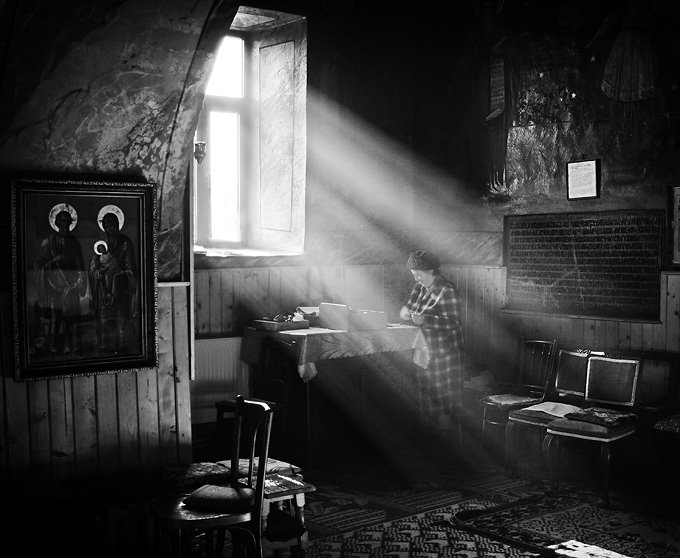
\includegraphics[width=1.4cm]{images/mission/room.png}};
        \node[inner sep=0pt, anchor=west] (whitehead) at ($(cmonitor) + (1.7,0)$)
            {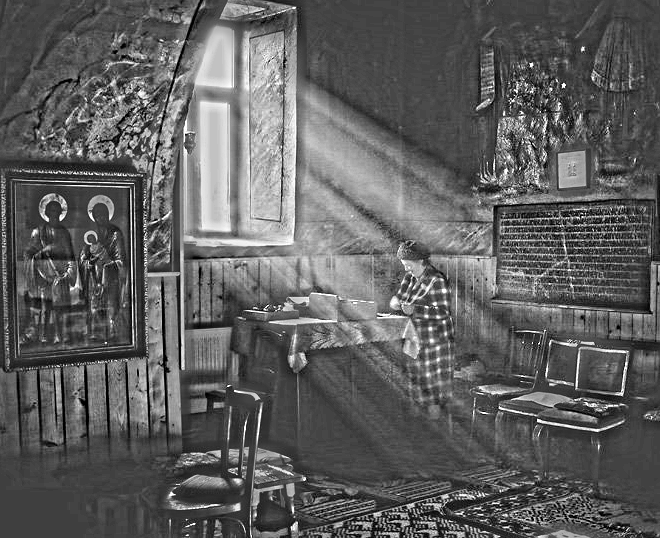
\includegraphics[width=1.4cm]{images/mission/room_fpga_vhdl_v20.png}};

        \node[] (eth) at ($(cmonitor) + (4.5, 1.0)$) {LAN};
        
        \draw[line width = 0.5mm] ($(eth) + (0,-1.0)$) ellipse (0.2cm and 0.5cm);
    \end{pgfonlayer}

    % FPGA box
    \begin{pgfonlayer}{main}
        \node[above = 0.2cm of com, xshift=-1.5cm] (fpga) { FPGA };
    \end{pgfonlayer}
    \begin{pgfonlayer}{foreground}
        \node (f_fpga) [draw=black, fill=gray!20, inner sep=20, fit={(com) (ip) (mem) (control) }] {};
    \end{pgfonlayer} 

    
    \path[draw,-{Latex[length=2.5mm]}] ($(mon.0) + (0,0.2)$) -- ($(com.180) + (0,0.2)$) node[near end, above] () {1.} ;
    \path[draw,{Latex[length=2.5mm]}-] ($(mon.0) + (0,-0.2)$) -- ($(com.180) + (0,-0.2)$) node[near end, below] () {8.} ;

    \path[draw,-{Latex[length=2.5mm]}] ($(control.180) + (0,0.2)$) -- ($(ip.0) + (0,0.2)$) node[midway, above] () {4.} ;
    \path[draw,{Latex[length=2.5mm]}-] ($(control.180) + (0,-0.2)$) -- ($(ip.0) + (0,-0.2)$) node[midway, below] () {5.} ;

    \path[draw,-{Latex[length=2.5mm]}] ($(control.90) + (-0.2,0)$) -- ($(mem.270) + (-0.2,0)$) node[midway, left] () {6.} ;
    \path[draw,{Latex[length=2.5mm]}-] ($(control.90) + (0.2,0)$) -- ($(mem.270) + (0.2,0)$) node[midway, right] () {3.} ;

    \path[draw,-{Latex[length=2.5mm]}] ($(com.0) + (0,0.2)$) -- ($(mem.180) + (0,0.2)$) node[midway, above] () {2.} ;
    \path[draw,{Latex[length=2.5mm]}-] ($(com.0) + (0,-0.2)$) -- ($(mem.180) + (0,-0.2)$) node[midway, below] () {7.} ;

\end{tikzpicture}
    \caption{Block diagram}
    \label{fig:blockdiagram}
\end{figure}



% ------------------------------------------------------------------------->>> %

% <<< ------------------------------------------------------- IMAGE PROCESSING %
\chapter{Image Processing}  \label{chapt:ip}
This chapter deals with the filter developed for the image. First the design flow of Vivado HLS is shown and then how an IP core is generated from a C/C++ code. Then the sobel algorithm is explained and how it was programmed. Finally, the scalability of the filter is discussed. 

\section{Design Flow}
In Vivado HLS it is possible to translate the C/C++ code into VHDL and generate an IP core for Vivado HLx. To ensure that the algorithm is correct, it can be validated in various steps. These steps are the design flow of Vivado HLS and are shown in figure \ref{fig:hls_design_flow}.
First of all, the C/C++ algorithm can be tested in a simulation. This requires a testbench in addition to the C/C++ algorithm. As soon as the algorithm works satisfyingly the design can be run through synthesis and generating a RTL design in VHDL. VHDL design can be verified in an RTL simulation. The RTL simulation must match the C/C++ simulation. If this is the case, an IP core can be generated from the VHDL code and used in the Vivado HLx \cite{vivado_hls}.
%IP Integrator erklären, Block Design, ...

\begin{figure}[tb!]
    \centering
    % \tikzsetnextfilename{system-overview}
\begin{tikzpicture}[
    rounded corners=0mm,
]
    %coordinates
    \coordinate (orig)      at (0,0);
    \coordinate (test)      at (-3,0);
    \coordinate (alg)       at (3,0);
    \coordinate (c_sim)     at (0,-1);
    \coordinate (c_synth)   at (0,-2);
    \coordinate (VHDL)      at (0,-3);
    \coordinate (rtl_sim)   at (0,-4);
    \coordinate (ip)        at (0,-5);
    \coordinate (hlx)       at (0,-6);

    %nodes
    \node[draw, fill=white, minimum width=4cm, minimum height=0.6cm, anchor=south, text width=3.8cm, align=center, rounded corners=3mm] (A) at (test) {C/C++ Testbench};
    \node[draw, fill=white, minimum width=4cm, minimum height=0.6cm, anchor=south, text width=3.8cm, align=center, rounded corners=3mm] (B) at (alg) {C/C++ Algorithm};
    \node[draw, fill=white, minimum width=4cm, minimum height=0.6cm, anchor=south, text width=3.8cm, align=center] (C) at (c_sim) {C/C++ Simulation};
    \node[draw, fill=white, minimum width=4cm, minimum height=0.6cm, anchor=south, text width=3.8cm, align=center] (D) at (c_synth) {C/C++ Synthesis};
    \node[draw, fill=white, minimum width=4cm, minimum height=0.6cm, anchor=south, text width=3.8cm, align=center, rounded corners=3mm] (E) at (VHDL) {VHDL};
    \node[draw, fill=white, minimum width=4cm, minimum height=0.6cm, anchor=south, text width=3.8cm, align=center] (F) at (rtl_sim) {RTL Simulation};
    \node[draw, fill=white, minimum width=4cm, minimum height=0.6cm, anchor=south, text width=3.8cm, align=center] (G) at (ip) {Package IP};
    \node[draw, fill=white, minimum width=4cm, minimum height=0.6cm, anchor=south, text width=3.8cm, align=center] (H) at (hlx) {Vivado HLx};

    %path
    \path [draw,-] (A) -- (B);
    \path[draw,-{Latex[length=2.5mm]}] (A) -| (C);
    \path[draw,-{Latex[length=2.5mm]}] (C.east) -- ++(3.5,0) |- (B.east);
    \path[draw,-{Latex[length=2.5mm]}] (C) -- (D);
    \path[draw,-{Latex[length=2.5mm]}] (D) -- (E);
    \path[draw,-{Latex[length=2.5mm]}] (E) -- (F);
    \path[draw,-{Latex[length=2.5mm]}] (E.west) -- ++(-0.5,0) |- (G.west);
    \path[draw,-{Latex[length=2.5mm]}] (F.east) -- ++(3.5,0) |- (B.east);
    \path[draw,-{Latex[length=2.5mm]}] (G) -- (H);


\end{tikzpicture}
    \caption{Vivado HLS design flow}
    \label{fig:hls_design_flow}
\end{figure}


\section{Requirements}
%Was ist für die Sobel-Edge-Detection notwendig und wie muessen die Pixelwerte vorliegen

The Sobel filter has some requirements. A grayscale image is required for edge detection. As already described in chapter \ref{chapt:mission_imageprocessing} the Sobel filter depends on its neighbor pixels. Therefore, the entire image does not have to be present. These are the most important requirements of this filter.


\section{Concept} \label{chapt:concept}
%Das Konzept des Programmierten Filters. Wie das Filter genau funktioniert. 

\begin{figure}[b]
    \centering
    \begin{adjustbox}{width=0.5\textwidth}
    	% \tikzsetnextfilename{system-overview}
\begin{tikzpicture}[
    rounded corners=0mm,
]
    %coordinates
    \coordinate (orig)      at (0,0);
    \coordinate (gray)      at (0,0);
    \coordinate (sob_x)     at (-2,-1);
    \coordinate (sob_y)     at (2,-1);
    \coordinate (grad)      at (0,-2);
    \coordinate (hyst)      at (0,-3);
    \coordinate (o_img)     at (0,-4);

    %nodes
    \node[draw, fill=white, minimum width=3cm, minimum height=0.6cm, anchor=south, text width=2.8cm, align=center] (A) at (gray) {Grayscale Image};
    \node[draw, fill=white, minimum width=3cm, minimum height=0.6cm, anchor=south, text width=2.8cm, align=center] (B) at (sob_x) {Sobel X};
    \node[draw, fill=white, minimum width=3cm, minimum height=0.6cm, anchor=south, text width=2.8cm, align=center] (C) at (sob_y) {Sobel Y};
    \node[draw, fill=white, minimum width=3cm, minimum height=0.6cm, anchor=south, text width=2.8cm, align=center] (D) at (grad) {Gradient};
    \node[draw, fill=white, minimum width=3cm, minimum height=0.6cm, anchor=south, text width=2.8cm, align=center] (E) at (hyst) {Hysteresis};
    \node[draw, fill=white, minimum width=3cm, minimum height=0.6cm, anchor=south, text width=2.8cm, align=center] (F) at (o_img) {Output Image};

    %path
    \path[draw,-{Latex[length=2.5mm]}] (A) -- (B);
    \path[draw,-{Latex[length=2.5mm]}] (A) -- (C);
    \path[draw,-{Latex[length=2.5mm]}] (B) -- (D);
    \path[draw,-{Latex[length=2.5mm]}] (C) -- (D);
    \path[draw,-{Latex[length=2.5mm]}] (D) -- (E);
    \path[draw,-{Latex[length=2.5mm]}] (E) -- (F);

    \node at (-1.5,-1.2) {\tiny Gx};
    \node at (1.5,-1.2) {\tiny Gy};

\end{tikzpicture}
    \end{adjustbox}
    \caption{Concept of the Sobel edge detection algorithm}
    \label{fig:sobel}
\end{figure}
	
The algorithm uses a convolution applying a 3x3 matrix, which generates a gradient image from the grayscale image. This is used to display high frequencies in the image with gray values. The areas of greatest intensity are where the brightness of the input image changes most rapidly and thus represents the largest edges. The concept of the Sobel algorithm is shown in figure \ref{fig:sobel}. 

Only a 3x3 section of the grayscale image $I$ is used for each pixel. With a 3x3 matrix, merely the nine neighboring pixels are used. The filter matrix are the approximations of the weighted derivatives in horizontal and vertical direction. \\

\noindent\begin{minipage}{.5\linewidth}

\textbf{Horizontal changes:}
\begin{equation}
    G_{x} = I * \begin{bmatrix}
                -1 & 0 & 1 \\ 
                -2 & 0 & 2 \\ 
                -1 & 0 & 1
                \end{bmatrix}
    \label{eq:gx_derivative}
\end{equation} \\

\end{minipage}%
\begin{minipage}{.5\linewidth}

\textbf{Vertical changes:}
\begin{equation}
    G_{y} = I * \begin{bmatrix}
                -1 & -2 & -1 \\ 
                0 & 0 & 0 \\ 
                1 & 2 & 1
                \end{bmatrix}
    \label{eq:gx_derivative}
\end{equation} \\

\end{minipage}


The gradient is calculated for each pixel of the image. The theory says that the root of squares of the two derivatives should be used:
\begin{equation}
    G = \sqrt{ G_{x}^{2} + G_{y}^{2}}
    \label{eq:g_square_root}
\end{equation}
\\

In order to save resources on the FPGA, the gradient can also be calculated with the absolute values of the derivatives:
\begin{equation}
    G = \left |G_{x}  \right | + \left |G_{y}  \right |
    \label{eq:g_abs}
\end{equation}
\\

The final stage of the Sobel edge detector is referred to as hysteresis. If the result $G$ is greater/lower than the maximum/minimum value, the result is set to this threshold value \cite{sobel_matrix}.


\section{Implementation}
The implementation of the Sobel edge detection is shown below. The code has the same sequence as shown in figure \ref{fig:sobel}. The edge detection is implemented as a function. For the function only the required pixels have to be passed. The two filter matrixes are defined in the header file. The return value is the gradient, in this case the variable \texttt{sum}. \\


Listing \ref{lst:matrix} contains the mirrored filter matrix for calculating horizontal changes. The matrix was mirrored because it is a convolution with the image.

\begin{minipage}{\textwidth}
\begin{lstlisting}[style=CStyle, caption=Filter matrix defined in header, label=lst:matrix]
// Filter-Matrix
static int sobel_x [3][3] = {{1,0,-1},
					  	  	 					 {2,0,-2},
												 		 {1,0,-1}};
\end{lstlisting}
\end{minipage}
\\

As can be seen in the filter matrix, the middle column has the weighting zero. Therefore, these pixels do not have to be included in the calculation and only six pixels have an impact on the calculation.

\begin{minipage}{\textwidth}
\begin{lstlisting}[style=CStyle , caption=Calculation of derivative, label=lst:derivative]
gx = 	sobel_x[0][0] * pixel_00 +
			sobel_x[1][0] * pixel_10 +
			sobel_x[2][0] * pixel_20 +
			sobel_x[0][2] * pixel_02 +
			sobel_x[1][2] * pixel_12 +
			sobel_x[2][2] * pixel_22;
\end{lstlisting}
\end{minipage}
\\

In this code section, the absolute value of each derivative is calculated and the gradient is generated.

\begin{minipage}{\textwidth}
\begin{lstlisting}[style=CStyle , caption=Evaluate the absolute value and the gradient, label=lst:gradient]
gx = gx < 0 ? -gx : gx; // abs(gx)
gy = gy < 0 ? -gy : gy; // abs(gy)
sum = gx + gy;
\end{lstlisting}
\end{minipage}
\\

Finally, the hysteresis is adjusted with an upper and lower threshold value. The calculated gradient can be returned as a new pixel.

\begin{minipage}{\textwidth}
\begin{lstlisting}[style=CStyle , caption=Threshold, label=lst:threshold]
sum = sum > 255 ? 255:sum; // max threshold
sum = sum < 0 ? 0 : sum; 	 // min threshold
\end{lstlisting}
\end{minipage}

\clearpage
\section{Scalability}
%Was wurde gemacht, damit der Filter im FPGA auf mehrere aufgeteilt werden kann.
In order to take advantage of the area on the FPGA and increase the throughput, the image can be split into blocks. A Sobel algorithm can be loaded with an image block to calculate it. Figure \ref{fig:impl_sobel} shows a model to calculate one row of pixels. On the left side is the input memory. A row of pixels is loaded into each one. Three pixels from every input memory are loaded into the Sobel filter. With these nine pixels a new pixel can be calculated and stored in the output memory.
This splitting into blocks guarantees a very simple scalability of the image within an FPGA and also on multiple FPGAs. The pixel data for a filter and the calculated pixel data must only be handled correctly. Figure \ref{fig:impl_sobel2} shows how this scalability can be used to implement multiple filters. 

\begin{figure}[h!]
    \centering
    \begin{adjustbox}{width=0.8\textwidth}
        % \tikzsetnextfilename{system-overview}
\begin{tikzpicture}[
    rounded corners=0mm,
]
    %coordinates
    \coordinate (orig)      at (0,0);
    \coordinate (sob)      at (0,-0.7);
    \coordinate (mem1)     at (-3.5,1);
    \coordinate (mem2)     at (-3.5,0);
    \coordinate (mem3)      at (-3.5,-1);
    \coordinate (mem4)      at (3.5,0);

    %nodes
    \node[draw, fill=white, minimum width=2cm, minimum height=2cm, anchor=south, text width=1.8cm, align=center] (A) at (sob) {Sobel Filter};
    \node[draw, fill=white, minimum width=3cm, minimum height=0.6cm, anchor=south, text width=2.8cm, align=center] (B) at (mem1) {Memory (row 0)};
    \node[draw, fill=white, minimum width=3cm, minimum height=0.6cm, anchor=south, text width=2.8cm, align=center] (C) at (mem2) {Memory (row 1)};
    \node[draw, fill=white, minimum width=3cm, minimum height=0.6cm, anchor=south, text width=2.8cm, align=center] (D) at (mem3) {Memory (row 2)};
    \node[draw, fill=white, minimum width=3cm, minimum height=0.6cm, anchor=south, text width=2.8cm, align=center] (E) at (mem4) {Memory (row 0)};

    %path
    \path[draw,-{Latex[length=2.5mm]}] (B.east) -- ++(0.5,0) |- ($(A.180) + (0,0.5)$);
    \path[draw,-{Latex[length=2.5mm]}] (C) -- (A);
    \path[draw,-{Latex[length=2.5mm]}] (D.east) -- ++(0.5,0) |- ($(A.180) + (0,-0.5)$);
    \path[draw,-{Latex[length=2.5mm]}] (A) -- (E);

\end{tikzpicture}
    \end{adjustbox}
    \caption{Implementation of the Sobel filter in the FPGA}
    \label{fig:impl_sobel}
\end{figure}

\begin{figure}[h!]
    \centering
    \begin{adjustbox}{width=0.8\textwidth}
    	% \tikzsetnextfilename{system-overview}
\begin{tikzpicture}[
    rounded corners=0mm,
]
    %coordinates
    \coordinate (orig)      at (0,0);
    \coordinate (sob)      at (0,-0.7);
    \coordinate (mem1)     at (-3.5,1);
    \coordinate (mem2)     at (-3.5,0);
    \coordinate (mem3)      at (-3.5,-1);
    \coordinate (mem4)      at (3.5,0);

    \coordinate (sob2)      at (0,-3.2);
    \coordinate (mem21)      at (-3.5,-3);
    \coordinate (mem22)      at (3.5,-2.5);

    \coordinate (sob3)      at (0,-5.7);
    \coordinate (mem31)      at (-3.5,-5.5);
    \coordinate (mem32)      at (3.5,-5);



    %nodes
    \node[draw, fill=white, minimum width=2cm, minimum height=2cm, anchor=south, text width=1.8cm, align=center] (A) at (sob) {Sobel Filter};
    \node[draw, fill=white, minimum width=3cm, minimum height=0.6cm, anchor=south, text width=2.8cm, align=center] (B) at (mem1) {Memory (row 0)};
    \node[draw, fill=white, minimum width=3cm, minimum height=0.6cm, anchor=south, text width=2.8cm, align=center] (C) at (mem2) {Memory (row 1)};
    \node[draw, fill=white, minimum width=3cm, minimum height=0.6cm, anchor=south, text width=2.8cm, align=center] (D) at (mem3) {Memory (row 2)};
    \node[draw, fill=white, minimum width=3cm, minimum height=0.6cm, anchor=south, text width=2.8cm, align=center] (E) at (mem4) {Memory (row 0)};

    \node[draw, fill=white, minimum width=2cm, minimum height=2cm, anchor=south, text width=1.8cm, align=center] (F) at (sob2) {Sobel Filter};
    \node[draw, fill=white, minimum width=3cm, minimum height=0.6cm, anchor=south, text width=2.8cm, align=center] (G) at (mem21) {Memory (row 3)};
    \node[draw, fill=white, minimum width=3cm, minimum height=0.6cm, anchor=south, text width=2.8cm, align=center] (H) at (mem22) {Memory (row 1)};

    \node[draw, fill=white, minimum width=2cm, minimum height=2cm, anchor=south, text width=1.8cm, align=center] (I) at (sob3) {Sobel Filter};
    \node[draw, fill=white, minimum width=3cm, minimum height=0.6cm, anchor=south, text width=2.8cm, align=center] (J) at (mem31) {Memory (row 4)};
    \node[draw, fill=white, minimum width=3cm, minimum height=0.6cm, anchor=south, text width=2.8cm, align=center] (K) at (mem32) {Memory (row 2)};


    %path
    \path[draw,-{Latex[length=2.5mm]}] (B.east) -- ++(0.5,0) |- ($(A.180) + (0,0.5)$);
    \path[draw,-{Latex[length=2.5mm]}] (C) -- (A);
    \path[draw,-{Latex[length=2.5mm]}] (D.east) -- ++(0.5,0) |- ($(A.180) + (0,-0.5)$);
    \path[draw,-{Latex[length=2.5mm]}] (A) -- (E);

    \path[draw,-{Latex[length=2.5mm]}] (C.east) -- ++(0.4,0) |- ($(F.180) + (0,0.5)$);
    \path[draw,-{Latex[length=2.5mm]}] (D.east) -- ++(0.3,0) |-  ($(F.180) + (0,0)$);
    \path[draw,-{Latex[length=2.5mm]}] (G) -- ($(F.180) + (0,-0.5)$);
    \path[draw,-{Latex[length=2.5mm]}] (F) -- (H);

    \path[draw,-{Latex[length=2.5mm]}] (D.east) -- ++(0.3,0) |- ($(I.180) + (0,0.5)$);
    \path[draw,-{Latex[length=2.5mm]}] (G.east) -- ++(0.2,0) |-  ($(I.180) + (0,0)$);
    \path[draw,-{Latex[length=2.5mm]}] (J) -- ($(I.180) + (0,-0.5)$);
    \path[draw,-{Latex[length=2.5mm]}] (I) -- (K);

    \node at (-1.575,0.3) [circle, fill, inner sep=0.7pt] {};
    \node at (-1.675,-0.7) [circle, fill, inner sep=0.7pt] {};
    \node at (-1.675,-2.2) [circle, fill, inner sep=0.7pt] {};
    \node at (-1.775,-2.7) [circle, fill, inner sep=0.7pt] {};



\end{tikzpicture}
    \end{adjustbox}
    \caption{Scalability of the Sobel filter in the FPGA}
    \label{fig:impl_sobel2}
\end{figure}



\section{Svynthesis}
Before optimizing the C/C++ code, the result must be analyzed. If the C/C++ code is synthesized without optimizations, the throughput will not be better than in a normal C/C++ program. For example, the compiler will process the loops sequentially. By adding attributes, directives, or pragmas the problem can be solved and the code can be adapted to hardware. For C/C++ code, pragmas are used to improve the throughput, latency or resources \cite{vivado_synthesis}. 


\subsection{Pragma}
Loops are often represented in the code to prepare and process the pixels in the proper order. The most important two pragmas for loops are \texttt{pipline} and \texttt{unroll} \cite{pragma}. These two functions improve the hardware's performance by exploiting the parallelism between loop iterations. \\

\textbf{Loop Piplining:} For a normal loop execution, processing is sequential and the next iteration of the loop cannot begin until the previous one is completed. Loop pipelining allows to start the next iteration in advance. 
As can be seen in figure \ref{fig:pipelining}, the loop has a latency of three clock cycles for the whole iteration. However, with the pragma \texttt{\#pragma HLS pipeline} the latency can be reduced to one clock cycle.
The pragma \texttt{pipline} is recursive and unrolls automatically all loops in the hierarchy. 
Loop pipelining is used if the data is not yet fully available. This means, as seen in figure \ref{fig:pipelining}, when for example it is necessary to load the data from a memory at first \cite{pragma}. \\


\begin{figure}[h!]
    \centering
    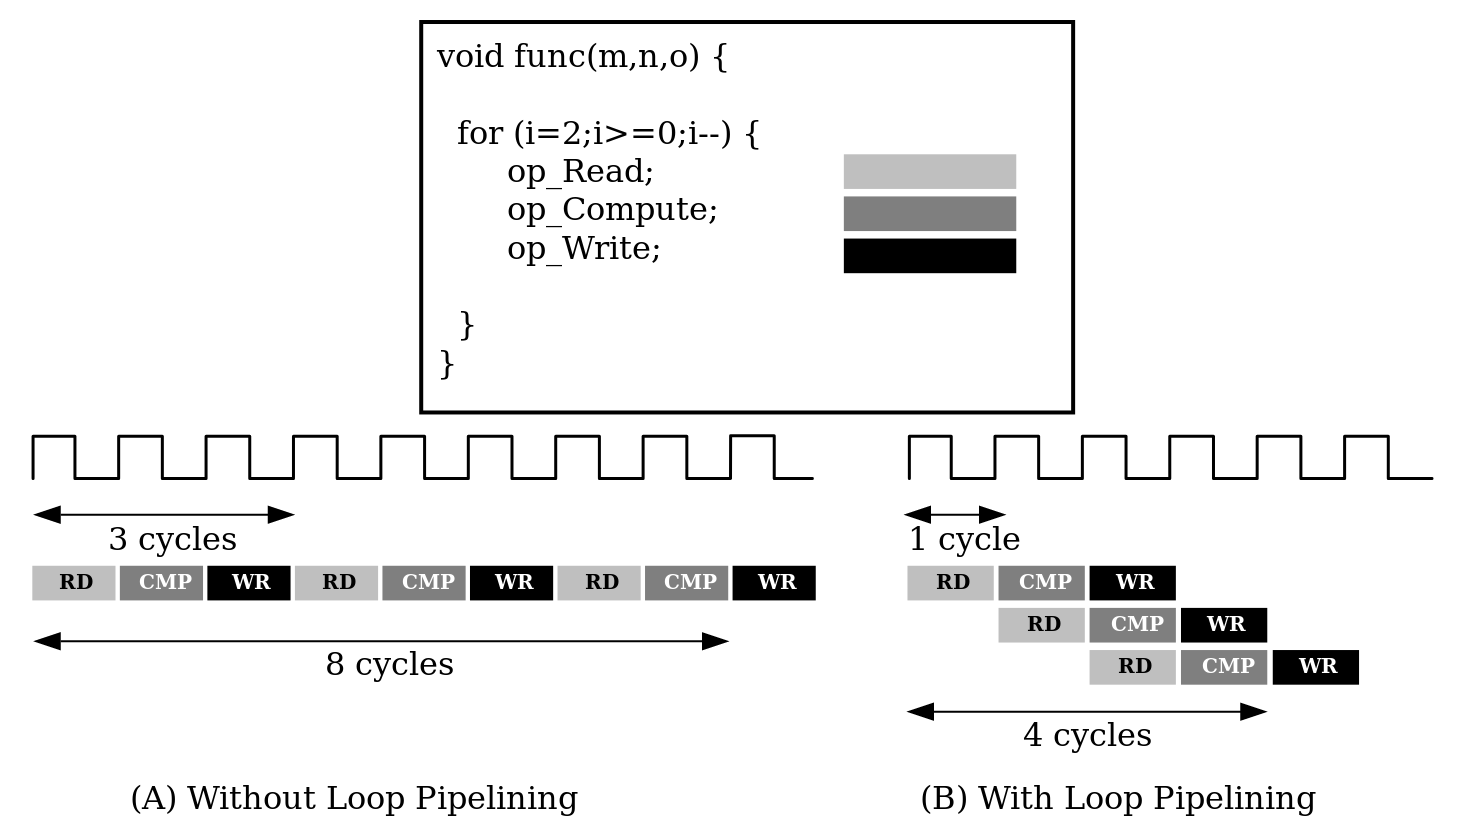
\includegraphics[width=0.8\textwidth]{images/image_processing/pipelining.png}
    \caption{Comparison of loop pipelinging \cite{pragma}}
    \label{fig:pipelining}
\end{figure}

\clearpage
\textbf{Loop Unrolling:} With the pragma \texttt{\#pragma HLS unroll} a loop can be parallelized. This means that the entire loop can be processed in parallel. With a factor, the parallelism can be controlled. By default, the entire loop is parallelized. 
Loop unrolling is used when the data is available and they are not loaded or already loaded for the entire loop \cite{pragma}. 
In this code section, the loop is parallelized with a factor of 2:

\begin{lstlisting}[style=CStyle , caption=Loop unrolling with a factor of 2 \cite{pragma}]
for(int i = 0; i < X; i++) {
  #pragma HLS unroll factor=2
  a[i] = b[i] + c[i];
}
\end{lstlisting}

The model of unrolling can be seen here:
\begin{lstlisting}[style=CStyle , caption=Loop unrolling with a factor of 2 \cite{pragma}]
for(int i = 0; i < X; i += 2) {
  a[i] = b[i] + c[i];
  if (i+1 >= X) break;
  a[i+1] = b[i+1] + c[i+1];
}
\end{lstlisting}


\subsection{Analysis}
Code analysis is important for optimizing code and improving performance. This section shows how to analyze a code. At Vivado HLS there is a report and graphical analysis to identify mistakes. 

\subsubsection*{Report Analysis}
The Sobel filter with and without pragmas is placed in contrast (see table \ref{tab:analysis}). The loop pragmas were optimized for throughput. With each new clock cycle a new iteration is started. As a result, the memory requirements increase as more variables have to be stored. 
The graphical analysis does not make any sense when processing without pragmas. Because of the nesting of multiple loops, the compiler can no longer work properly. In the next example, the graphical analysis makes much more sense .\\

\begin{table}[h!]
    \centering
    \begin{tabular}{ l l l }
    	\toprule
         & {without Pragma} & {with Pragma} \\ 
        \midrule
        Latency & 23'471 - 31'631 & 515 \\
        Throughput & 0.018 Pixel / Clk & 1 Pixel / Clk \\ 
        FF & 2783 & 3451 \\ 
        LUT & 2574 & 2512 \\ 
        \bottomrule
    \end{tabular}
    \caption{Report analysis (iterations: 510)}
    \label{tab:analysis}
\end{table}

\clearpage
\subsubsection*{Graphical Analysis}
Graphical analysis in the Vivado HLS is very useful. The goal was to improve memory access and thereby increasing throughput. In the first programming an error occurred and during the analysis the following figure \ref{tab:wrong_code} appeared. The figure shows that at each iteration it accesses the memory twice. Two clock cycles are required to read out one word from a BRAM. In the first, the address is sent to the BRAM and in the second, the data is read out \cite{bram}. In figure \ref{tab:wrong_code} however, the addressing to the BRAM occures in clock 1 (C1). In Clock 2 (C2) the pixels are read out and the second addressing follows for the pixels which are read out in Clock 3 (C3). However, there should be only one memory access at each iteration. At an iteration size of 510, this resulted in a latency of 1024 clock cycles. \\

By positioning the memory access in front of the loop, these two memory accesses could be avoided with each iteration. The result of the analysis is in figure \ref{tab:correct_code}. The new latency has been reduced to 515 clock cycles but the initialization was bigger, because the memory access is before the loop (C0 and C1).


\begin{table}[h!]
\setlength{\aboverulesep}{0pt}
\setlength{\belowrulesep}{0pt}
\centering
\begin{tabular}{lllll|l|llll}
\hline
\multicolumn{1}{|l|}{C0} & \multicolumn{1}{l|}{C1} & \multicolumn{1}{l|}{C2} & \multicolumn{1}{l|}{C3} & C4 & C5 & \multicolumn{1}{l|}{C6} & \multicolumn{1}{l|}{C7} & \multicolumn{1}{l|}{C8} & \multicolumn{1}{l|}{C9} \\ \hline
\multicolumn{1}{|l|}{\cellcolor[HTML]{9B9B9B}{\color[HTML]{FFFFFF} Init}} & \multicolumn{1}{l|}{\cellcolor[HTML]{9B9B9B}{\color[HTML]{FFFFFF} RD}} & \multicolumn{1}{l|}{\cellcolor[HTML]{9B9B9B}{\color[HTML]{FFFFFF} RD}} & \multicolumn{1}{l|}{\cellcolor[HTML]{9B9B9B}{\color[HTML]{FFFFFF} RD}} & \cellcolor[HTML]{FFFFFF}{\color[HTML]{333333} CALC} & \cellcolor[HTML]{9B9B9B}{\color[HTML]{FFFFFF} WR} & {\color[HTML]{FFFFFF} } & {\color[HTML]{FFFFFF} } &  &  \\ \cmidrule{1-8}
{\color[HTML]{FFFFFF} } & {\color[HTML]{FFFFFF} } & \multicolumn{1}{l|}{{\color[HTML]{FFFFFF} }} & \multicolumn{1}{l|}{\cellcolor[HTML]{9B9B9B}{\color[HTML]{FFFFFF} RD}} & \cellcolor[HTML]{9B9B9B}{\color[HTML]{FFFFFF} RD} & \cellcolor[HTML]{9B9B9B}{\color[HTML]{FFFFFF} RD} & \multicolumn{1}{l|}{\cellcolor[HTML]{FFFFFF}{\color[HTML]{333333} CALC}} & \multicolumn{1}{l|}{\cellcolor[HTML]{9B9B9B}{\color[HTML]{FFFFFF} WR}} &  &  \\ \cmidrule{4-10}
{\color[HTML]{FFFFFF} } & {\color[HTML]{FFFFFF} } & {\color[HTML]{FFFFFF} } &  &  & \cellcolor[HTML]{9B9B9B}{\color[HTML]{FFFFFF} RD} & \multicolumn{1}{l|}{\cellcolor[HTML]{9B9B9B}{\color[HTML]{FFFFFF} RD}} & \multicolumn{1}{l|}{\cellcolor[HTML]{9B9B9B}{\color[HTML]{FFFFFF} RD}} & \multicolumn{1}{l|}{\cellcolor[HTML]{FFFFFF}{\color[HTML]{333333} CALC}} & \multicolumn{1}{l|}{\cellcolor[HTML]{9B9B9B}{\color[HTML]{FFFFFF} WR}} \\ \cmidrule{6-10}
\end{tabular}
\caption{The wrong code with three iterations in the loop}
\label{tab:wrong_code}
\end{table}


\begin{table}[h!]
\setlength{\aboverulesep}{0pt}
\setlength{\belowrulesep}{0pt}
\centering
\begin{tabular}{llll|llll}
\hline
\multicolumn{1}{|l|}{C0} & \multicolumn{1}{l|}{C1} & \multicolumn{1}{l|}{C2} & \multicolumn{1}{l|}{C3} & \multicolumn{1}{l|}{C4} & \multicolumn{1}{l|}{C5} & \multicolumn{1}{l|}{C6} & \multicolumn{1}{l|}{C7} \\ \hline
\multicolumn{1}{|l|}{\cellcolor[HTML]{9B9B9B}{\color[HTML]{FFFFFF} Init}} & \multicolumn{1}{l|}{\cellcolor[HTML]{9B9B9B}{\color[HTML]{FFFFFF} Init}} & \multicolumn{1}{l|}{\cellcolor[HTML]{9B9B9B}{\color[HTML]{FFFFFF} RD}} & \multicolumn{1}{l|}{\cellcolor[HTML]{9B9B9B}{\color[HTML]{FFFFFF} RD}} & \multicolumn{1}{l|}{\cellcolor[HTML]{FFFFFF}{\color[HTML]{333333} CALC}} & \multicolumn{1}{l|}{\cellcolor[HTML]{9B9B9B}{\color[HTML]{FFFFFF} WR}} & {\color[HTML]{FFFFFF} } & {\color[HTML]{FFFFFF} } \\ \cmidrule{1-7}
{\color[HTML]{FFFFFF} } & {\color[HTML]{FFFFFF} } & \multicolumn{1}{l|}{{\color[HTML]{FFFFFF} }} & \multicolumn{1}{l|}{\cellcolor[HTML]{9B9B9B}{\color[HTML]{FFFFFF} RD}} & \multicolumn{1}{l|}{\cellcolor[HTML]{9B9B9B}{\color[HTML]{FFFFFF} RD}} & \multicolumn{1}{l|}{{\color[HTML]{333333} CALC}} & \multicolumn{1}{l|}{\cellcolor[HTML]{9B9B9B}{\color[HTML]{FFFFFF} WR}} & {\color[HTML]{FFFFFF} } \\ \cmidrule{4-8}
{\color[HTML]{FFFFFF} } & {\color[HTML]{FFFFFF} } & {\color[HTML]{FFFFFF} } &  &  \multicolumn{1}{l|}{\cellcolor[HTML]{9B9B9B}{\color[HTML]{FFFFFF} RD}} & \multicolumn{1}{l|}{\cellcolor[HTML]{9B9B9B}{\color[HTML]{FFFFFF} RD}} & \multicolumn{1}{l|}{\cellcolor[HTML]{FFFFFF}{\color[HTML]{333333} CALC}} & \multicolumn{1}{l|}{\cellcolor[HTML]{9B9B9B}{\color[HTML]{FFFFFF} WR}} \\ \cmidrule{5-8}
\end{tabular}
\caption{The correct code with three iterations in the loop}
\label{tab:correct_code}
\end{table}



% ------------------------------------------------------------------------->>> %

% <<< ------------------------------------------------ COMMUNICATION & CONTROL %
% ==============================================================================
%
%                             Dataflow
%
% ==============================================================================
\chapter{Dataflow} \label{chapt:dataflow}

% ==============================================================================
%                             Communication
% ==============================================================================
\section{Communication}

% ==============================================================================
%                             Acknowledge
% ==============================================================================
\subsection{Acknowledge}

% ==============================================================================
%                             Retransmission
% ==============================================================================
\subsection{Retransmission}

% ==============================================================================
%                             Interface
% ==============================================================================
\subsection{Interface}

% ==============================================================================
%                             Control
% ==============================================================================
\section{Control}

% ==============================================================================
%                             Concept
% ==============================================================================
\subsection{Concept}

\subsection{Implementation (HLS)}


\subsubsection*{IF-Statement} \label{ch:data:if}

\begin{minipage}{\textwidth}
\begin{lstlisting}[style=CStyle, caption=Buffer switching reloading without else statement, label=lst:buf_false]
if( (outPpBuf == ppBufA) && (ms_pctr < (inLineSize-PIN_PONG_BUF_SIZE)) ) {
    if(!ppBufBrdy) {
        ...
    }
}
if( (outPpBuf == ppBufB) && (ms_pctr < (inLineSize-PIN_PONG_BUF_SIZE)) ) {
    if(!ppBufArdy) {
        ...
    }
}
\end{lstlisting}
\end{minipage}

\begin{minipage}{\textwidth}
\begin{lstlisting}[style=CStyle, caption=Buffer switching reloading with else statement, label=lst:buf_right]
if (ms_pctr < (inLineSize-PIN_PONG_BUF_SIZE)) {
	if( (outPpBuf == ppBufA)  ) {
		if(!ppBufBrdy) {
			...
		}
	}
	else {
		if(!ppBufArdy) {
			...
		}
	}
}
\end{lstlisting}
\end{minipage}

\subsection{Implementation (VHDL)}

% ------------------------------------------------------------------------->>> %

% <<< ------------------------------------------------------------ SCALABILITY %
% ==============================================================================
%
%                             Scalability
%
% ==============================================================================
\chapter{Scalability} \label{chapt:scalability}
The code for this project is written from the beginning with the possibility to
scale it up in mind. The main idea being that the throughput can be increased.
Scalability in regard to this project can be divided into two terms:
\begin{itemize}
    \item Inside FPGA
    \item Across multiple FPGAs
\end{itemize}

In the following sections these two aspects are dissected theoretically.

\section{Inside FPGA}
Every FPGA has a given amount of ressources (LUTs, memory and so forth, as
described in table \ref{tab:XC7A200T}). The inside FPGA scalability aims towards
optimal usage of these ressources. Before methods for scalability can be
compared it must be clarified what can be scaled. The \gls{diip} project
consists of three main parts. The communication, controller and image processing
parts. The communication part is only implemented once to handle the
communication to the PC and therefore can not be scaled. The image processing
part however can be implemented multiple times inside the FPGA to increase
throughput. Therefore the conrtoller part splits up the incomming image data and
distributes it to the image processing cores. To summarize the inside FPGA
scalability:
\begin{itemize}
    \item Implement the communication part once
    \item Implement the image processing part as many times as the available
    ressources allow it
    \item Adapt the controller to distribute data accross the processing cores
\end{itemize}

Figure \ref{fig:insidefpgascaleconceptbd} clarifies the concept. Note that all
image processing cores are equal.

\begin{figure}[tb!]
    \centering
    \begin{adjustbox}{max width=\linewidth}
        % \tikzsetnextfilename{system-overview}
\begin{tikzpicture}[
    rounded corners=0mm,
]
    %coordinates
    \coordinate (corig)      at (0,0);
    \coordinate (cmonitor)   at (0,0);
    \coordinate (ccom)       at (5,0);
    \coordinate (cip)        at (10,0);


    %nodes

    \begin{pgfonlayer}{main}

        \node[draw, fill=white, minimum width=3cm, minimum height=2cm, anchor=west, text width=2.8cm, align=center] (com) at (ccom) {Controller and Image Cache};

        \node[draw, fill=white, minimum width=3cm, minimum height=1cm, anchor=west, text width=2.8cm, align=center, above =1cm of com] (commu) {Communication};

        \node[draw, fill=white, minimum width=3cm, minimum height=1cm, anchor=west, text width=2.8cm, align=center, right = 1cm of com, yshift=2.5cm] (ip1) {Image\\Processing};
        \node[draw, fill=white, minimum width=3cm, minimum height=1cm, anchor=west, text width=2.8cm, align=center, right = 1cm of com, yshift=1.0cm] (ip2) {Image\\Processing};
        \node[draw, fill=white, minimum width=3cm, minimum height=1cm, anchor=west, text width=2.8cm, align=center, right = 1cm of com, yshift=-0.5cm] (ip3) {Image\\Processing};
        
        \node[circle,fill=black,minimum size=0.2cm,inner sep=0pt, below = 0.3cm of ip3] (dt1)  {};
        \node[circle,fill=black,minimum size=0.2cm,inner sep=0pt, below = 0.2cm of dt1] (dt2)  {};
        \node[circle,fill=black,minimum size=0.2cm,inner sep=0pt, below = 0.2cm of dt2] (dt3)  {};

        % \node[] (eth) at ($(cmonitor) + (4.5, 1.0)$) {LAN};
        
        % \draw[line width = 0.5mm] ($(eth) + (0,-1.0)$) ellipse (0.2cm and 0.5cm);
    \end{pgfonlayer}

    % FPGA box
    \begin{pgfonlayer}{main}
        \node[above = 2.4cm of com, xshift=-1.2cm] (fpga) { FPGA };
    \end{pgfonlayer}
    \begin{pgfonlayer}{foreground}
        \node (f_fpga) [draw=black, fill=gray!20, inner sep=10, fit={(com) (ip1) (ip2) (ip3) (dt2) (dt1) (dt3)}] {};
    \end{pgfonlayer} 

    
    \path[draw,{Latex[length=4mm]}-{Latex[length=4mm]},line width =1mm] ($(commu.180) + (-1.5,0)$) -- ($(commu.180) + (0,0)$) 
        node[near start, left, anchor=east,xshift=-0.5cm] () {PC} ;
    \path[draw,{Latex[length=4mm]}-{Latex[length=4mm]},line width =1mm] ($(com.90) + (0,0)$) -- ($(commu.270) + (0,0)$) node[near start, left, anchor=east,xshift=-0.5cm] () {} ;

    \path[draw,{Latex[length=2.5mm]}-{Latex[length=2.5mm]}] 
        ($(com.0) + (0,0.7)$) -| ($(ip1.180) + (-0.6,0)$) -- ($(ip1.180) + (0,0)$)
         node[near start, left, anchor=east,xshift=-0.5cm] () {} ;
    \path[draw,{Latex[length=2.5mm]}-{Latex[length=2.5mm]}] 
        ($(com.0) + (0,0.1)$) -| ($(ip2.180) + (-0.4,0)$) -- ($(ip2.180) + (0,0)$) 
        node[near start, left, anchor=east,xshift=-0.5cm] () {} ;
    \path[draw,{Latex[length=2.5mm]}-{Latex[length=2.5mm]}] ($(com.0) + (0,-0.5)$) -- ($(ip3.180) + (0,0)$) node[near start, left, anchor=east,xshift=-0.5cm] () {} ;

    % Legend
    \path[draw,{Latex[length=4mm]}-{Latex[length=4mm]},line width =1mm] 
        ($(ip1.0) + (1,0)$) -- ($(ip1.0) + (2,0)$) 
        node[near end, right, anchor=west,xshift=0.5cm] () {High bandwidth} ;
    \path[draw,{Latex[length=2.5mm]}-{Latex[length=2.5mm]}] 
        ($(ip1.0) + (1,-0.50)$) -- ($(ip1.0) + (2,-0.50)$) 
        node[near end, right, anchor=west,xshift=0.5cm] () {Low bandwidth} ;

\end{tikzpicture}
    \end{adjustbox}
    \caption{Block diagram of a inside FPGA scaled solution}
    \label{fig:insidefpgascaleconceptbd}
\end{figure}

Now that the concept is clarified, two possible solutions are compared to
distribute the image data accross the image processing cores, proposal A and B.
They differ in the way in what order the data is sent to the FPGA and how it is
cached inside the FPGA. For each proposal the following metrics are calculated.

\begin{description}
    \item[Initial size $s_i$]\hfill \\
    The number of pixels that have to be sent to the FPGA before beginning
    interational operation.
    \item[Iteration size $s_r$]\hfill \\
    How many pixels that have to be sent to start a new iteration.
    \item[Store size $s_s$]\hfill \\
    How many pixels have to be cached inside the FPGA.
    \item[Number of inits per image $n_i$]\hfill \\
    Denotes the number of initial data transfers of size $s_i$ have to be made
    per image.
    \item[Total tx size $s_{tx}$]\hfill \\
    The total number of pixels sent to the FPGA to calculate one image.
    \item[Number of image processing cores $N$]\hfill \\
    The number of image processing cores implemented on the FPGA.
\end{description}


\begin{table}[tb!]
    \centering
    \begin{tabular}{p{0.45\textwidth} p{0.45\textwidth}}
        \toprule
        \multicolumn{1}{c}{Proposal A} & \multicolumn{1}{c}{Proposal B} \\
        \midrule
            \begin{adjustbox}{max width=0.4\textwidth}
                % \tikzsetnextfilename{system-overview}
\begin{tikzpicture}[
    rounded corners=0mm,
    triangle/.style = {fill=blue!20, regular polygon, regular polygon sides=3 },
    node rotated/.style = {rotate=180},
    border rotated/.style = {shape border rotate=180}
]
    %coordinates
    \coordinate (orig)      at (0,0);

    \begin{pgfonlayer}{main}
        
        % Braces
        % \draw [line width=0.5mm,decorate,decoration={brace,amplitude=10pt},xshift=-4pt,yshift=0pt] (9.5,5) -- (9.5,0) node [black,midway,xshift=0.5cm,anchor=west] {Window length};
        % \draw [line width=0.5mm,decorate,decoration={brace,amplitude=10pt},xshift=-0pt,yshift=0pt] (8,-0.5) -- (0,-0.5) node [black,midway,yshift=-0.5cm,anchor=north] {Image width};
        
        % Center pixel
        % \draw[black,line width=0.5mm] (2,2) rectangle (3,3);
        
        % Window sizes
        \draw[blue,line width=0.6mm] (0,4) rectangle (3,7);
        \draw[red,line width=0.6mm,dashed] (0,3) rectangle (3,6);
        % \draw[black,line width=0.6mm,dotted] (0,2) rectangle (3,5);
        % resulting lines
        \draw[cyan,line width=0.6mm] (1,5) rectangle (5,6);
        \draw[magenta,line width=0.6mm,dashed] (1,4) rectangle (5,5);
        % \draw[black,line width=0.3mm,dotted] (1,3) rectangle (5,4);

        % Arrows
        % \path[draw,-{Latex[length=2.5mm]}] (0,7.5) -- (4,7.5) 
        %     node[near start, above] () {iterate} ;
        \path[draw,-{Latex[length=3.5mm]},line width=0.4mm] (-0.5,7) -- (-0.5,3) 
            node[near start, above,rotate=270] () {send data} ;

        % Axis
        % \foreach \x in {0,1,2,3,4}
        %     \node[anchor=north] at ($(-0.5,5)-(0,\x)$)  {$\x$};

    \end{pgfonlayer}

    % Foreground
    \begin{pgfonlayer}{foreground}
        
    \end{pgfonlayer} 

    % Background
    \begin{pgfonlayer}{background}
        % Init pixels
        \draw[fill=gray!20] (0,3) rectangle (6,7);
        % Iter pixels
        \draw[pattern=north east lines, pattern color=gray!60] (0,2) rectangle (6,3);
        % Grid
        \draw[step=1cm,black,thin] (0,0) grid (6,7);
    \end{pgfonlayer} 

\end{tikzpicture}
            \end{adjustbox}
        & 
            \begin{adjustbox}{max width=0.4\textwidth}
                % \tikzsetnextfilename{system-overview}
\begin{tikzpicture}[
    rounded corners=0mm,
    triangle/.style = {fill=blue!20, regular polygon, regular polygon sides=3 },
    node rotated/.style = {rotate=180},
    border rotated/.style = {shape border rotate=180}
]
    %coordinates
    \coordinate (orig)      at (0,0);

    \begin{pgfonlayer}{main}
        
        % Braces
        % \draw [line width=0.5mm,decorate,decoration={brace,amplitude=10pt},xshift=-4pt,yshift=0pt] (9.5,5) -- (9.5,0) node [black,midway,xshift=0.5cm,anchor=west] {Window length};
        % \draw [line width=0.5mm,decorate,decoration={brace,amplitude=10pt},xshift=-0pt,yshift=0pt] (8,-0.5) -- (0,-0.5) node [black,midway,yshift=-0.5cm,anchor=north] {Image width};
        
        % Center pixel
        % \draw[black,line width=0.5mm] (2,2) rectangle (3,3);
        
        % Window sizes
        \draw[blue,line width=0.6mm] (0,4) rectangle (3,7);
        \draw[red,line width=0.6mm,dashed] (0,3) rectangle (3,6);
        % \draw[black,line width=0.6mm,dotted] (0,2) rectangle (3,5);
        % resulting lines
        \draw[cyan,line width=0.6mm] (1,5) rectangle (8,6);
        \draw[magenta,line width=0.6mm,dashed] (1,4) rectangle (8,5);
        % \draw[black,line width=0.3mm,dotted] (1,3) rectangle (5,4);

        % Arrows
        \path[draw,-{Latex[length=2.5mm]},line width=0.4mm] (0,7.5) -- (4,7.5) 
            node[near start, above] () {send data} ;
        % \path[draw,-{Latex[length=3.5mm]},line width=0.4mm] (-0.5,7) -- (-0.5,3) 
        %     node[near start, above,rotate=270] () {init} ;

        % Axis
        % \foreach \x in {0,1,2,3,4}
        %     \node[anchor=north] at ($(-0.5,5)-(0,\x)$)  {$\x$};

    \end{pgfonlayer}

    % Foreground
    \begin{pgfonlayer}{foreground}
        
    \end{pgfonlayer} 

    % Background
    \begin{pgfonlayer}{background}
        % Init pixels
        \draw[fill=gray!20] (0,3) rectangle (3,7);
        % Iter pixels
        \draw[pattern=north east lines, pattern color=gray!60] (3,3) rectangle (4,7);
        % Grid
        \draw[step=1cm,black,thin] (0,0) grid (9,7);
    \end{pgfonlayer} 

\end{tikzpicture}
            \end{adjustbox}
        \\
        % \multicolumn{1}{c}{caption}&
        % \multicolumn{1}{c}{caption}
        % \\
        \multicolumn{2}{c}{
            \begin{adjustbox}{max width=0.8\textwidth}
                % \tikzsetnextfilename{system-overview}
\begin{tikzpicture}[
    rounded corners=0mm,
    triangle/.style = {fill=blue!20, regular polygon, regular polygon sides=3 },
    node rotated/.style = {rotate=180},
    border rotated/.style = {shape border rotate=180}
]
    %coordinates
    \coordinate (orig)      at (0,0);

    \begin{pgfonlayer}{main}
        
        % Init pixels
        \draw[fill=gray!20] (0,0) rectangle (1,0.6);
        \node[anchor=west] at (1.2,0.3)  {Init data};

        \draw[pattern=north east lines, pattern color=gray!60] (3,0) rectangle (4,0.6);
        \node[anchor=west] at (4.2,0.3)  {Iteration data};

        \draw[blue,line width=0.6mm] (7,0) rectangle (8,0.6);
        \node[anchor=south] at (7.5,0.1) {$c0$};
        \draw[red,line width=0.6mm,dashed] (8.5,0) rectangle (9.5,0.6);
        \node[anchor=south] at (9,0.1) {$c1$};
        % \draw[black,line width=0.4mm,dotted] (10,0) rectangle (11,0.6);
        \node[anchor=west] at (9.7,0.3)  {Image processing cores 0 and 1};
        % Iter pixels
        % \draw[pattern=north east lines, pattern color=gray!60] (3,2) rectangle (4,7);

        \draw[cyan,line width=0.6mm] (7,-1) rectangle (8,-0.4);
        \node[anchor=south] at (7.5,-1) {$c0$};
        \draw[magenta,line width=0.6mm,dashed] (8.5,-1) rectangle (9.5,-0.4);
        \node[anchor=south] at (9.0, -1) {$c1$};
        \node[anchor=west] at (9.7,-0.7)  {Processed output pixels};

        \node[anchor=south west] at (0, -1) {$N_{cx}$};
        \node[anchor=south west] at (1.2, -1) {$N$th output pixel of core $x$};
    \end{pgfonlayer}

    % Foreground
    \begin{pgfonlayer}{foreground}
        
    \end{pgfonlayer} 

    % Background
    \begin{pgfonlayer}{background}
        % Grid
        % \draw[step=1cm,gray,thin] (0,0) grid (6,7);
    \end{pgfonlayer} 

\end{tikzpicture}
            \end{adjustbox}
        }
        \\\midrule
        \textbf{Concept} & \\
        Image data is sent line wise. Each image processing core handles one
        input line, starts as soon as enough data is transfered and jumps $N$ lines
        downwards after completion.
        &
        Image data is sent coloumn wise with $w_l+(N-1)$ pixels per coloumn. All
        image processing cores start processing at the same time and progress
        $N$ lines downwards after completion.
        \\\midrule
        \textbf{Initial size} & \\
        {\( 
            s_i = i_w(w_l+(N-1))
        \)}
        &
        {\( 
            s_i = w_l(w_l+(N-1))
        \)}
        \\\midrule
        \textbf{Iterarion size} & \\
        {\( 
            s_r  = i_w
        \)}
        &
        {\( 
            s_r  = w_l+(N-1)
        \)}
        \\\midrule
        \textbf{Store size} & \\
        {\( 
            s_s  = i_w(w_l+(N-1))
        \)}
        &
        {\( 
            s_s  = w_l(w_l+(N-1))
        \)}
        \\\midrule
        \textbf{Number of inits per image} & \\
        {\( 
            n_i  = 1
        \)}
        &
        {\( 
            n_i  = \frac{1}{N}(i_w-w_l+1)
        \)}
        \\\midrule
        \textbf{Total tx size} & \\
        {\( 
            s_{tx}  = i_w \cdot i_h
        \)}
        &
        {\( 
            s_{tx}  = n_i s_i + (i_w-w_l)s_r n_i
        \)}
        \\
        \bottomrule
    \end{tabular}
    \caption{Inside FPGA scalability proposals}
    \label{tab:insidefpgascalability}
\end{table}

Before comparing the two proposals another metric has to be taken into
consideration: The effective throughput of the image processing core. The way
the wallis filter works is that it requires a neighbourhood of pixels. For each
line the core processes, the initial neighbourhood has to be sent. Equation
\ref{eq:theomaxvhdlwallise} derived in appendix 
\ref{app:derivations:theomaxvhdlwallis} is used to calculate the effective
throughput $b_r$ of a Wallis filter core. To simplify, the image height $i_h$ is
considered to be much larger than the window length $w_l$ and therefore the
equation can be noted as shown in equation \ref{eq:vhdlwallismaxb}. Using the
throughput of the VHDL Wallis filter implementation ($b_w=125Mp/s$) and the
window length $w_l=21$ the effective bandwidth $b_r$ is calculated:

\begin{align}
    b_r  & \approx \frac{b_w}{w_l} = 5.95 Mp/s
    \label{eq:vhdlwallismaxb}
\end{align}

Under the assumption that the real throughput $b_r$ scales proportionally with the
number of image processing cores implemented, equation 
\ref{eq:scaledrealttotalhroughput} can be noted to represent the total image
processing throughput $b_t$.

\begin{align}
    b_t  & = N \cdot b_r
    \label{eq:scaledrealttotalhroughput}
\end{align}

Considering the maximum throughput of the Gigabit-Ethernet connection of
$b_e=125MB/s$ \footnote{True Ethernet throughput is less than 125MB/s
considering packet overhead} equation \ref{eq:maxethernetthrouhgput} can be derived to calculate the
maximum number of image processing cores that can be implemented before the
Ethernet communication link is saturated.

\begin{align}
    b_e \geq b_t = N \cdot b_r \Rightarrow N \leq \frac{b_e}{b_r} \approx 
    \frac{b_e w_l}{b_w} = w_l = 21
    \label{eq:maxethernetthrouhgput}
\end{align}

To calculate the free memory the results from \ref{asdf} \todo{ref to ressource
VHDL} are dissected to calculate the available memory. Table \ref{tab:membudget}
lists the required block memory usage.

\begin{table}[h!]
    \centering
    \begin{tabular}{l r}
        \toprule
        Item & BRAM tiles \\
        \midrule
        Total available & 365 \\
        TEMAC support & -2 \\
        UDP IP Core & -1.5 \\
        21 divider generators & -10.5 \\
        21 Wallis cores & -10.5 \\
        \midrule
        Free & 340.5\\
        \bottomrule
    \end{tabular}
    \caption{FPGA block memory budget}
    \label{tab:membudget}
\end{table}

After using up memory for the communication and image processing cores, 340.5
block RAM tiles with 36Kb each results in 1'496KB of remaining block RAM that
can be used for image caching. Table \ref{tab:parsum} summarizes the
parameters that are used to compare the two inside FPGA scale proposals.

\begin{table}[h!]
    \centering
    \begin{tabular}{l r l}
        \toprule
        Parameter & Value & Description\\
        \midrule
        $N$ & 21 & Number of image processing cores to implement \\
        $s_b$ & 1'532KB & Block memory storage available for cache \\
        $w_l$ & 21 & Window length of the Wallis filter \\
        \bottomrule
    \end{tabular}
    \caption{Parameter summary}
    \label{tab:parsum}
\end{table}

Now the two proposals can be put to contrast. Starting with figure 
\ref{fig:sca:compfixheight} the two proposals are compared against each other
with an input image of fixed height and variable with. This was chosen because
with the main limiting factor being \gls{bramtile} usage, the store size $s_s$ has to
be observed and it is for both proposals independant of image height $i_h$. The
two proposals can be differentiated in that proposal A is optimized for low tx
size $s_{tx}$ (and therefore optimized for throughput) while proposal B requires
buch less memory (area optimized). 
\\
The BRAM usage 


\begin{figure}[tb!]
    \centering
    \begin{adjustbox}{max width=\linewidth}
        % Preamble: 
% \pgfplotsset{width=7cm,compat=1.5.1}
\begin{adjustbox}{max width=1\linewidth}
\begin{tabular}{c c}
\begin{tikzpicture}
    % \pgfplotsset{
    %     scaled x ticks=base 10:3
    % }
    \begin{axis}[
            % height=9cm,
            % width=9cm,
            grid=major,
            title=BRAM usage with variable image width,
            xlabel=$i_w \lbrack p \rbrack$,
            ylabel=BRAM tile usage,
            legend pos=north west,
            % xtick={10,20,...,70},
            every axis plot/.append style={thick}
        ]

            \addplot[mark=none,blue] coordinates {
                (8192, 72.88888889)
                (16384,145.7777778)
                (32768,291.5555556)
                (64536,583.1111111)
            };
            \addlegendentry{prosoal A}

            \addplot[mark=none,red] coordinates {
                (8192, 0.186848958)
                (16384,0.186848958)
                (32768,0.186848958)
                (64536,0.186848958)
            };
            \addlegendentry{prosoal B}
            
            \addplot[mark=none, black, dashed] coordinates {(8192,340.5) (64536,340.5)};
            \addlegendentry{available}
    \end{axis}
\end{tikzpicture}
&
\begin{tikzpicture}
    \begin{axis}[
            % height=9cm,
            % width=9cm,
            grid=major,
            title=Tx size with variable image width,
            xlabel=$i_w \lbrack p \rbrack$,
            ylabel=$s_{tx} \lbrack p \rbrack$,
            legend pos=north west,
            % xtick={10,20,...,70},
            every axis plot/.append style={thick}
        ]

            \addplot[mark=none,blue,smooth] coordinates {
                (8192, 198967296)
                (16384, 402653184)
                (32768, 805306368)
                (64536, 1610612736)
            };
            \addlegendentry{prosoal A}

            \addplot[mark=none,red,smooth] coordinates {
                (8192, 127795360)
                (16384, 523288576)
                (32768, 2094497792)
                (64536, 8383365120)
            };
            \addlegendentry{prosoal B}
            
            \addplot[mark=none, black, dashed] coordinates {(8192,198967296) (64536,1610612736)};
            \addlegendentry{image size}
    \end{axis}
\end{tikzpicture}
\end{tabular}
\end{adjustbox}

    \end{adjustbox}
    \caption{Comparing proposals width variable image width ($w_l=N=21$,
    $i_h=24'576$)}
    \label{fig:sca:compfixheight}
\end{figure}


\section{Across FPGA}
text

\section{Usecase}


% ------------------------------------------------------------------------->>> %

% <<< ----------------------------------------------- BENCHMARK & VERIFICATION %
% ==============================================================================
%
%                             Verification & Benchmark
%
% ==============================================================================
\chapter{Verification \& Benchmark} \label{chapt:ver_bench}
With the image processing an dataflow parts implemented, they can be verified
and benchmarked. The next chapters hold the verification process of both the
image processing part and the dataflow part. After both components are verified
they are benchmarked as one unity against a computer based implementation in
chapter \ref{ch:benchmark}.


% ==============================================================================
%
%                             Verification
%
% ==============================================================================
\section{Verification} \label{ch:verification}
The verification process ensures that all components work as expected. It is
split into the image processing and dataflow parts. They were tested
independantly to reduce complexity and simulation time. The system as a unity is
then tested in chapter \ref{ch:benchmark} benchmark.

% ==============================================================================
%
%                             Image Processing
%
% ==============================================================================
\subsection{Image Procession}\label{ch:verification:imageprocessing}
The verification of the image processing is validated with two different 
methods. Firstly, an image is processed with the Wallis filter and compared 
with a reference image. The reference image is generated from a C/C++ program 
which calculates using floating point calculations. In the second aspect the 
throughput is validated. \\
The devices under validation (DUV) are two written in Vivado HLS using C/C++ 
and one VHDL version. The Vivado HLS versions differ in the input stream. One 
has an 8 bit AXI4-Stream and the other one has a 256 bit AXI4-Stream input. The
VHDL is an 8 bit AXI4-Stream.

\subsubsection*{Image Comparsion}
During the verification an image is processed with the Wallis filter. The Wallis filter is run on the computer as a C/C++ program and has floating point variables. This Wallis filtering is used as a reference image. Two images (room and mountain), added in the appendix \ref{app:images_wallis}, are available as reference images. \\
The reference images are passed through the DUV and compared with the reference images. The root-mean-square error (RMSE) serves as a rule. The RMSE indicates how well the  Wallis filtered image deviates on average from the reference image \cite{rmse}. The parameters for the Wallis filter, which were used for the images, can be found in table \ref{tab:parameter}.

\begin{table}[tb!]
    \centering
    \begin{tabular}{l l l l l}
        \toprule
        Image & Brightness & Contrast & Global Mean & Global Variance \\
        \midrule
        room \ref{fig:ref_room} & 0.5 & 0.8125 & 127 & 3600 \\
        mountain \ref{fig:ref_mountain} & 0.5 & 0.8125 & 127 & 3600 \\
        \bottomrule
    \end{tabular}
    \caption{Parameters for the Wallis filter}
    \label{tab:parameter}
\end{table}



Table \ref{tab:rmse_room} lists the RMSE values of the room image and the RMSE values of the mountain image in the table \ref{tab:rmse_mountain}. They represent the deviation from the reference image in percent. The deviation from the C/C++ program with the 8 bit AXI4 stream and the 256 bit AXI4 stream does not differ from each other. A total deviation of 0.32\% has been measured in the room image. This corresponds to an intensity value of 0.816 in the range of 0 - 255. There is also only a deviation of 0.33\% in the mountain image. The GHDL verification is with 1.23\% respectively ??? already much higher. The intensity deviates by 3.14 pixels. This is due to the fact that in the VHDL code the mean value and the variance are not exactly calculated in contrast to the HLS versions. \todo{Begruednung!!!}

\begin{table}[tb!]
    \centering
    \begin{tabular}{l l l l}
        \toprule
        DUV & C/C++ Simulation (HLS) & RTL Simulation (HLS) & GHDL \\
        \midrule
        C/C++ 8 bit (HLS) & 0.32\% & 0.32\% & -\\
        C/C++ 256 bit (HLS) & 0.32\% & 0.32\% & - \\
        VHDL 8 bit & - & - & 1.23\% \\
        \bottomrule
    \end{tabular}
    \caption{RMSE of the Wallis filter verification of the room image}
    \label{tab:rmse_room}
\end{table}

\begin{table}[tb!]
    \centering
    \begin{tabular}{l l l l}
        \toprule
        DUV & C/C++ Simulation (HLS) & RTL Simulation (HLS) & GHDL \\
        \midrule
        C/C++ 8 bit (HLS) & 0.33\% & 0.33\% & - \\
        C/C++ 256 bit (HLS) & 0.33\% & 0.33\% & - \\
        VHDL 8 bit & - & - & 0.49\% \\
        \bottomrule
    \end{tabular}
    \caption{RMSE of the Wallis filter verification of the mountain image}
    \label{tab:rmse_mountain}
\end{table}



\subsubsection*{Throughput}
During verification, the throughput of the Wallis filter will also be evaluated. For this purpose, the throughput at the input of the filter is displayed. This means how many pixels per clock are loaded into the Wallis filter. Again, the three different methods (HLS 8 bit, HLS 256 bit \& VHDL 8 bit) of the Wallis filter are compared. The table \ref{tab:throughput} lists the three different methods. The 8 bit versions should have a throughput of one pixel per clock, this is 125Mp/s. But the HLS 8 bit version only reached 21 pixels in 86 clocks. This results in a throughput of 30.5Mp/s. This is 4 time slower than the theoretical value. This has to do with the fact that the division requires 23 clocks and that the loop cannot be pipelined by reading the pixels (see chapter \ref{ch:hls:div} and \ref{ch:ip:axi}). For this reason the 256 bit version was developed. This has a theoretical maximum of 2625Mp/s. A throughput of 21 pixels could be achieved in 11 clock cycles. This is equivalent to 238.6Mp/s. in relation to the 8 bit version only a better throughput of a factor of 7.8 could be achieved. The limiting factor is still the division. With the VHDL version the theoretical maximum of 125Mp/s has been reached.

\begin{table}[tb!]
    \centering
    \begin{tabular}{l l l l}
        \toprule
        DUV & Target [pxl/clk] & Actual [pxl/clk]  & Throughput [Mp/s]\\
        \midrule
        C/C++ 8 bit (HLS) & 1 & 21/86 & 30.5\\
        C/C++ 256 bit (HLS) & 21 & 21/11 & 238.6 \\
        VHDL 8 bit & 1 & 1 & 125 \\
        \bottomrule
    \end{tabular}
    \caption{Throughput of the Wallis filter related to the input pixels}
    \label{tab:throughput}
\end{table}


% ==============================================================================
%
%                             Dataflow
%
% ==============================================================================
\subsection{Dataflow}\label{ch:verification:dataflow}
The dataflow part is again divided into two parts, the communication and
controller parts. While in the communication part only the most recent version
is tested (reffering to chapter \ref{chapt:dataflow} explaining the solotion
A and B with streaming interface), both versions of the controller are verified.

\subsubsection*{Communication}
The communication part was in a large part taken from the last semester project
and was been thoroughly tested and validated in the project report 
\cite{p5report}. The three new implemented features are verified in this
chapter. They consist of:
\begin{itemize}
    \item Acknowledge
    \item User registers
    \item Stream interface
\end{itemize}

\vspace{1ex}
\textbf{Acknowledge:} To test the acknowledge function, a file was sent to the
FPGA from the computer
and the Ethernet traffic monitored with Wireshark Netowrk Protocol Analyzer.
Wiresharks packet dissections are exported to a json file that was then analyzed
using the \texttt{uftcheck} utility. It was written to analyze network pacekts
for UFT transfers. The first lines of output yielded:

    \begin{adjustbox}{max width=1.7\textwidth}
\begin{minipage}{2\linewidth}
    \begin{lstlisting}[
        % basicstyle=\small, %or \small or \footnotesize etc.
        % columns=fullflexible,
        % frame=single,
        % breaklines=false,
        % style=CStyle, 
        % caption=ack buffer allocation, 
        % label=lst:ackbufalloc
        ]
+------+----------------------+----------------------+-----+------------+------+------+
| Pack |         From         |          To          | D/C |  Control   | TCID | SEQ  | 
+------+----------------------+----------------------+-----+------------+------+------+
|  1   | 192.168.5.10 (50719) | 192.168.5.9 (42042)  |  C  |  FT Start  |  12  | 1036 |
|  2   | 192.168.5.10 (50719) | 192.168.5.9 (42042)  |  D  |            |  12  |  0   |
|  3   | 192.168.5.9 (42042)  | 192.168.5.10 (50719) |  C  | ACK packet |  12  |  0   |
|  5   | 192.168.5.10 (50719) | 192.168.5.9 (42042)  |  D  |            |  12  |  1   |
|  6   | 192.168.5.9 (42042)  | 192.168.5.10 (50719) |  C  | ACK packet |  12  |  1   |\end{lstlisting}
\end{minipage}
\end{adjustbox}

The sending PC starts a file transmission with a file transfer start packet and
the first data packet. The next packet (3) is comming from the FPGA to the PC
and acknowledges the first data packet (sequence 0). To verify that all packets
are acknowledged, the sending program reports an acknowledge status after the
files has been sent. 

\begin{minipage}{\linewidth}
    \begin{lstlisting}[
        % basicstyle=\small, %or \small or \footnotesize etc.
        % columns=fullflexible,
        % frame=single,
        % breaklines=false,
        % style=CStyle, 
        % caption=ack buffer allocation, 
        % label=lst:ackbufalloc
        ]
$ ./sender 192.168.5.9 42042 payload/cat.jpg
UFT Sender demo
destination 192.168.5.9:42042
HURRAY! All 1036 packets have been acknowledged.
time elapsed: 1.18s Speed: 0.859 MB/s Size: 1.012 MB\end{lstlisting}
\end{minipage}

\vspace{1ex}
\textbf{User register:} To test wether the user registers can be written and are
output correctly by the communication core, a integrated logic analyzer (ILA)
was used. An ILA can be configured on the FPGA to record internal signals. The
results are transferred to the PC over USB and displayed in \gls{vivadohlx}. 


\subsubsection*{Controller}

% ==============================================================================
%
%                             Benchmark
%
% ==============================================================================
\section{Benchmark}\label{ch:benchmark}


% ------------------------------------------------------------------------->>> %

% <<< ------------------------------------------------------------- CONCLUSION %
% ==============================================================================
%
%                             Conclusion
%
% ==============================================================================
\chapter{Conclusion}
In this last chapter the project results are briefly summarized and
a short outlook for possible future work is given.

% ==============================================================================
%
%                             IP
%
% ==============================================================================
\section{Image Processing}
A new image processing core was implemented that locally optimizes contrast 
(Wallis filter). Multiple implementations have been validated and compared.
Using high level synthesis to describe an algorithm has proven that the desired
operation can be achieved in little time. Nevertheless the theoretical possible
throughput could not be achieved. The main reason being that the dataflow was
not described well enough in C/C++ language to achieve the desired throughput.
Therefore a VHDL implementation was written that processes pixels at 125Mp/s and
uses less than three percent of FPGA ressources.

% ==============================================================================
%
%                             Dataflow
%
% ==============================================================================
\section{Dataflow}
The existing communication core was extended with acknowledge, user registers
and AXI4-Stream interfaces. The new image processing algorithm requires the
input data in a specific order. Therefore a controller was implemented using two
different design flows. The HLS approach showed that complex interfaces such as
AXI4 can be controller with a few lines of code and that state machines can be
implemented as well. The unfavourable memory management and the lack of high
throughput
led to the implementation of a VHDL based controller and memory management unit.
It caches necessary image data to obviate multiple image transmission and can
support the full throughput of the image processing core.

% ==============================================================================
%
%                             Overall
%
% ==============================================================================
\section{Overall}
The final product called \gls{diip} is is based on the VHDL implementations of
image processing and dataflow parts. Images can be sent from the PC to the FPGA
where
the Wallis operation is applied and the image is sent back. Image data
throughput of up to 4.1MB/s have been measured. The system is designed with
scalability in mind. A dedicated theoretical examination shows that if the
image processing core was implemented 21 times in the FPGA the full bandwidth of
gigabit Ethernet could be used to process image data yielding 125MB/s
throughput. Furthermore if multiple FPGAs were used, the total throughput would
scale proportional to the number of FPGAs used.

% ==============================================================================
%
%                             Working with High Level Synthesis
%
% ==============================================================================
\section{Working with High Level Synthesis}
The time spent on working with \gls{vivadohls} has shown several advantages and
disadvantages. It has shown that thinking close to hardwre is crucial. Using
C/C++ as language is a trap to fall back and think of the code as if it would be
executed sequentially. The function to be implemented should be split into
building blocks the same way as it would be done using a hardware description
language. If the code was written with the exact same line of thought as a HDL
approach, then the same throughput should be achievable. And if that is managed,
HLS would bring significant advantages like the simple implementation of complex
interfaces (e.g. AXI4) and the reduced time in testbench development.

% ==============================================================================
%
%                             Future Work
%
% ==============================================================================
\section{Future Work}
This scalability is proven on paper and can now be implemented onto the FPGA.
The controller core can be extended to send the data to multiple Wallis filter
cores. After writing a computer application that can handle the fast transfer
speeds the true benefit of using FPGA for image processing can be shown in
praxis. Because the data transfer is Ethernet based a cluster of FPGAs can be
built up to compete against high performance CPU and GPU based image processing
pipelines. Another method to increase throughput would be to implement a VHDL
256bit image processing core that would be able to process 21 pixels per clock
cycle and produce one pixel per clock cycle on the output. This would omit the
scalability inside the FPGA because the Ethernet link would already be
saturated. Furthermore the HLS implementations could be improved by describing
the dataflow more hardware oriented and proove that using HLS the same
throughput can be achieved as when using a hardware description language.


% ------------------------------------------------------------------------->>> %

%%%%%%%%%%%%%%%%%%%%%%%%%%%%%%%%%%%%%%%%%%%%%%%%%%%%%%%%%%%%%%%%%%%%%%%%%%%%%%%%
%                        	    R E S O U R C E  							   %
%%%%%%%%%%%%%%%%%%%%%%%%%%%%%%%%%%%%%%%%%%%%%%%%%%%%%%%%%%%%%%%%%%%%%%%%%%%%%%%%
\phantomsection

%%%%%%%%%%%%%%%%%%%%%%%%%%%%%%%%%%%%%%%%%%%%%%%%%%%%%%%%%%%%%%%%%%%%%%%%%%%%%%%%
%                             G L O S S A R Y                                  %
%%%%%%%%%%%%%%%%%%%%%%%%%%%%%%%%%%%%%%%%%%%%%%%%%%%%%%%%%%%%%%%%%%%%%%%%%%%%%%%%
% \clearpage{\pagestyle{empty}\cleardoublepage}
\printglossaries
% \clearpage{\pagestyle{empty}\cleardoublepage}

% <<< ----------------------------------------------------------- BIBLIOGRAPHY %
% \addcontentsline{toc}{chapter}{Bibliography}
\bibliographystyle{IEEEtran}
\bibliography{bibtex}
% ------------------------------------------------------------------------->>> %

% <<< -------------------------------------------------------- LIST of FIGURES %
\listoffigures
\listoftables
% \lstlistoflistings

\clearpage{\pagestyle{empty}\cleardoublepage}
% ------------------------------------------------------------------------->>> %
 

%%%%%%%%%%%%%%%%%%%%%%%%%%%%%%%%%%%%%%%%%%%%%%%%%%%%%%%%%%%%%%%%%%%%%%%%%%%%%%%%
%                             A P P E N D I C E S							   %
%%%%%%%%%%%%%%%%%%%%%%%%%%%%%%%%%%%%%%%%%%%%%%%%%%%%%%%%%%%%%%%%%%%%%%%%%%%%%%%%
\clearpage{\pagestyle{empty}\cleardoublepage}
\begin{appendix}
% ==============================================================================
%
%                             Appendices
%
% ==============================================================================
\chapter{Appendices}\label{chp:appendices}

\section{Aufgabenstellung 2018 P6 Distributed FPGA} \label{app:aufgabenstellung}
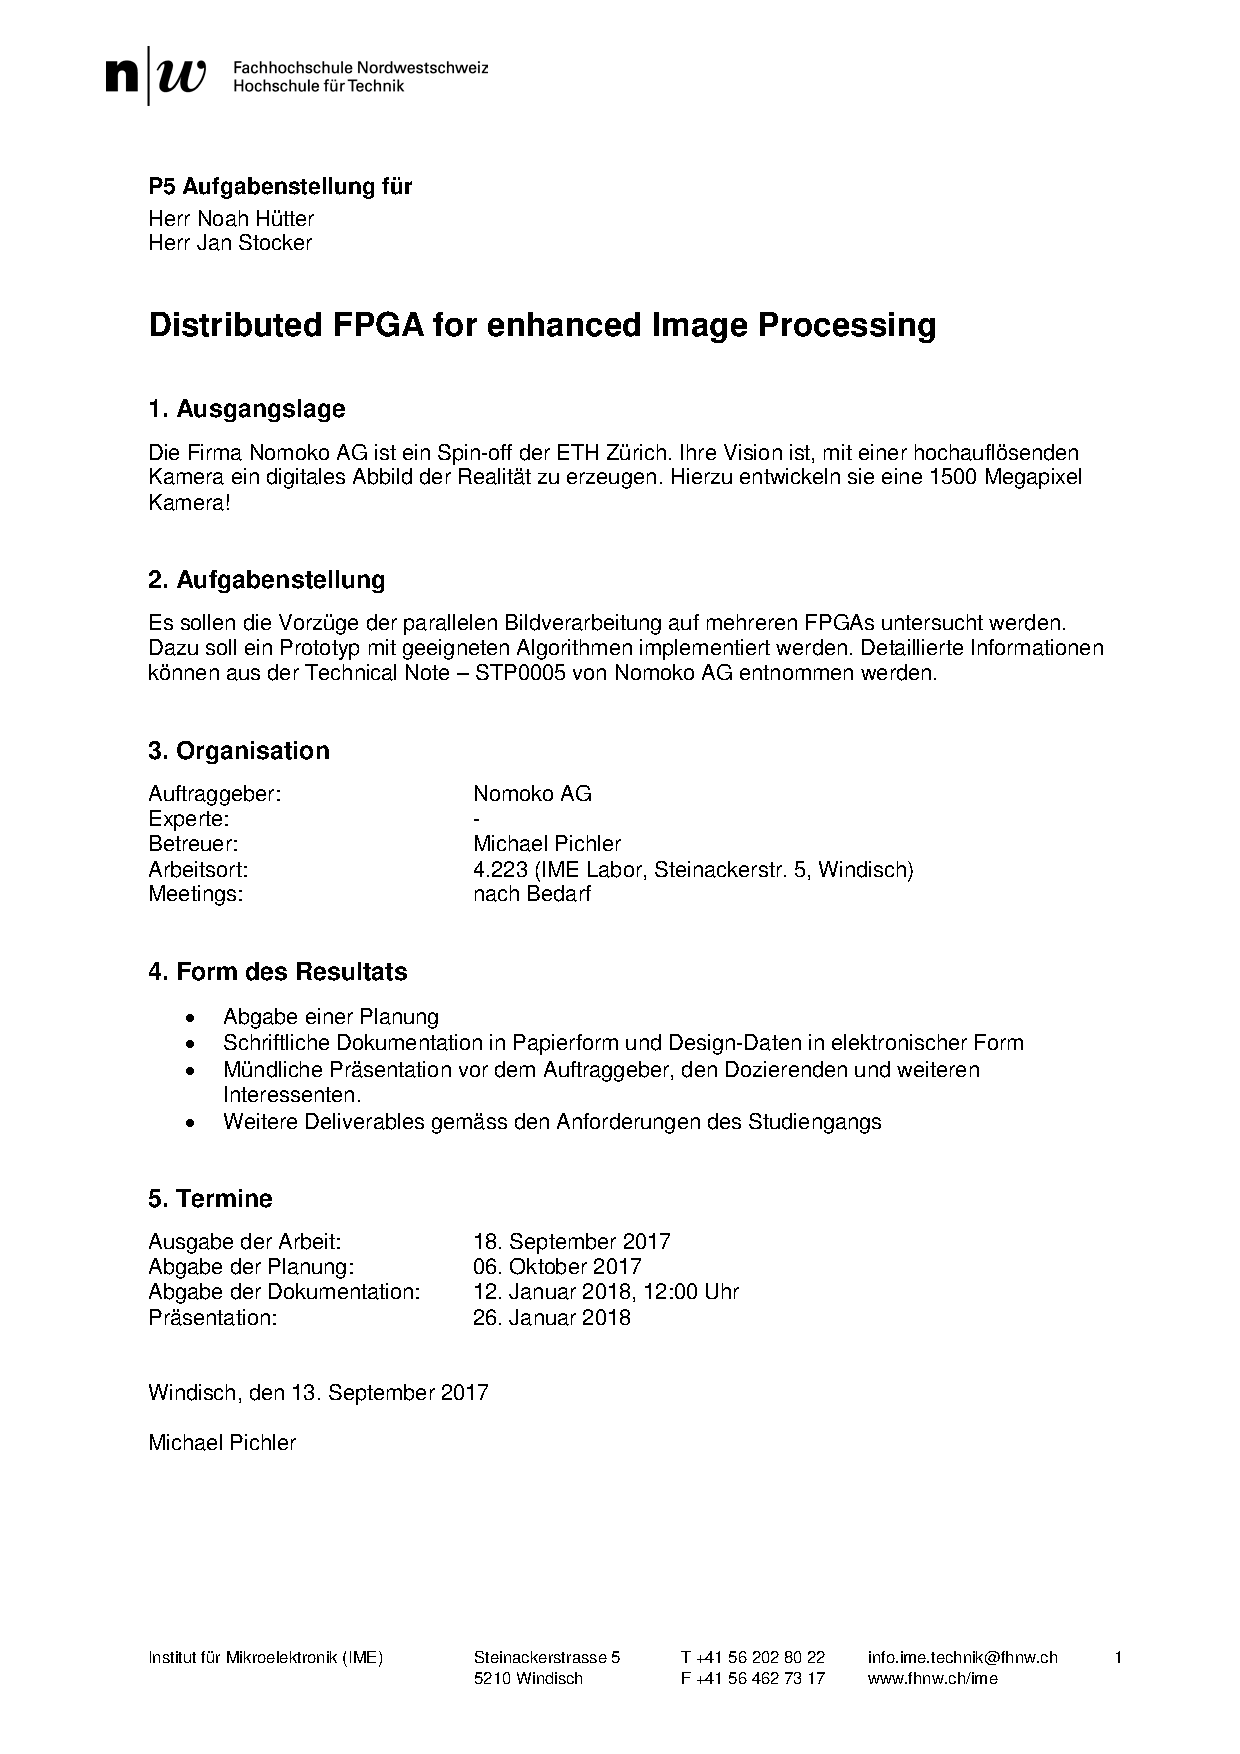
\includepdf[pages=-,scale=1,linktodoc=false]{appendices/Aufgabenstellung_2017_P5_Distributed_FPGA_comb.pdf}

\section{Technicial requirements} \label{app:technicial_requirements}

\includepdf[pages=-,scale=1,linktodoc=false]{appendices/technical_requirements_P6.pdf}

\section{Data types of the Wallis filter} \label{app:datatypes}
\begin{table}[H]
    \centering
    \begin{tabularx}{\textwidth}{l l}
        \toprule
        Name & Description \\
        \midrule
        iPxl & 			Pixel from the input image which is calculated \\
        g\_Mean &  		Global mean of the output image \\
        g\_Var &  		Global variance of the output image \\
        n\_Mean &		Mean of the neighborhood \\
        n\_Var &  		Variance of the neighborhood \\
        brightness & 	Brightness factor \\
        contrast & 		Contrast factor \\
        b\_gMean &  	Multiplication of brightness and global mean\\
        ci\_gVar &  	Multiplication of (1 - contrast) and global variance\\
        tmp\_Num &  	Temporary numerator of the division without contrast\\
        num &   		Numerator of the division with contrast\\
        c\_nVar &  		Multiplication of contrast and neighborhood variance\\
        bi\_nMean &  	Multiplication of (1 - brigthness) and neighborhood mean\\
        den\_Var & 		Denumerator of the division \\
        rec & 			Variable has value 1 to calculate a reciprocal division\\
        den & 			Result of the reciprocal division\\
        div &  			Result of the entire Wallis filter division\\
        w\_pixel &  	Output pixel from the Wallis filter\\
        \bottomrule
    \end{tabularx}
    \caption{Description of data types in the Wallis filter division}
\end{table}

\clearpage

\section{UDP File Transfer} \label{app:uftspec}

\includepdf[pages=-,scale=1,linktodoc=false]{appendices/UDP_File_Transfer.pdf}

\section{UDP file transfer calculation} \label{app:uftcalc}
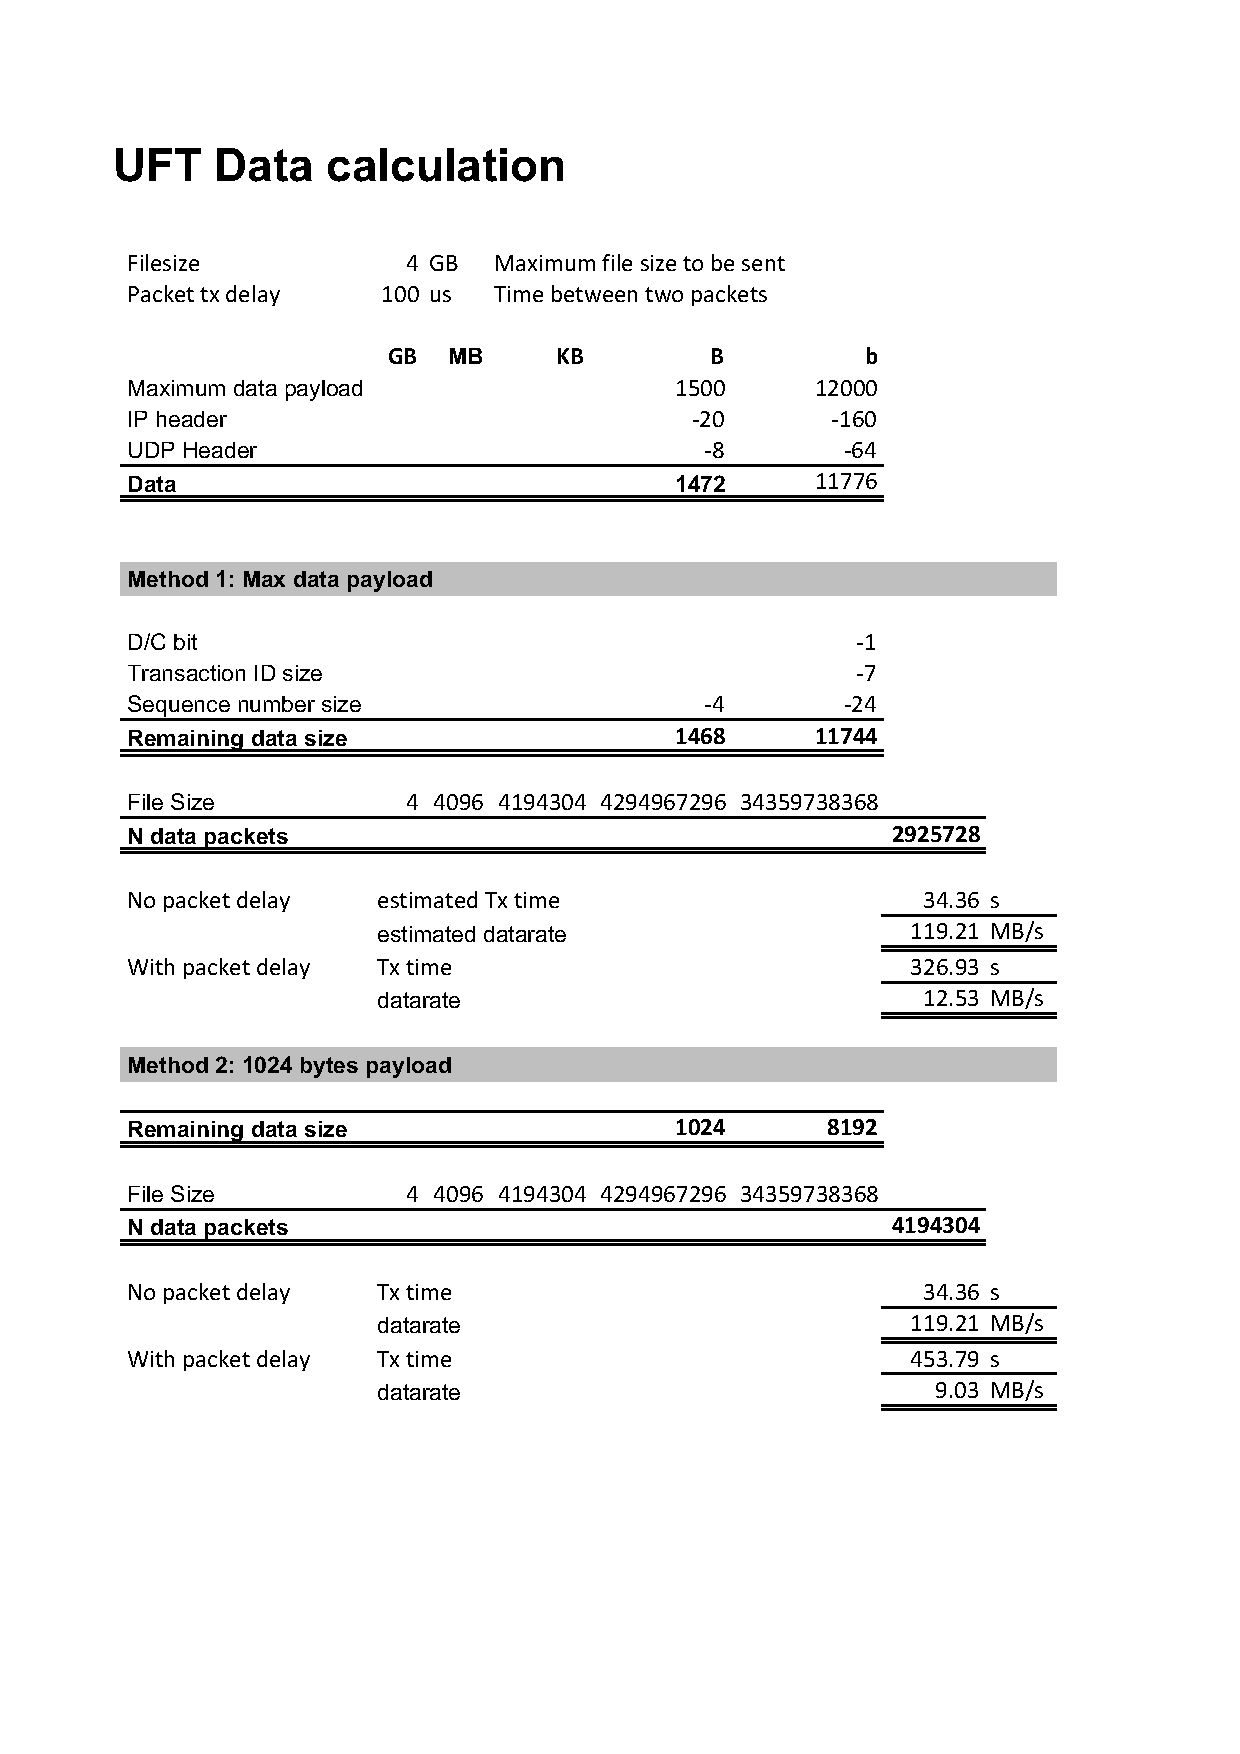
\includepdf[pages=-,scale=1,linktodoc=false]{appendices/uftcalc.pdf}

\section{Images for Wallis filter} \label{app:images_wallis}
\begin{figure}[H]
    \centering
    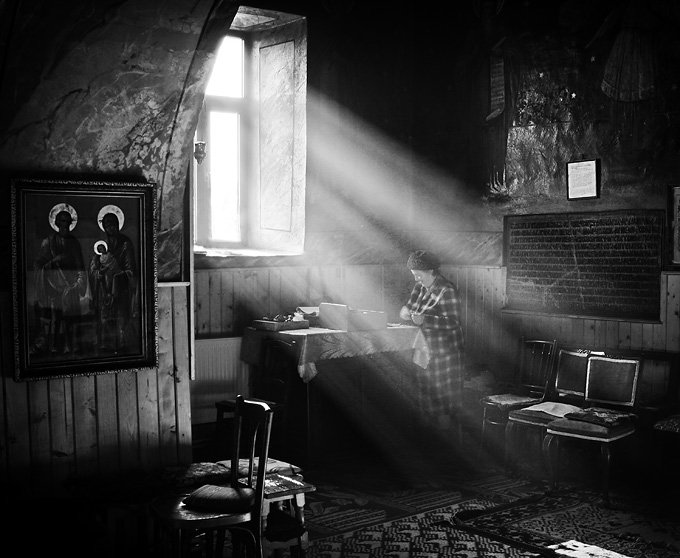
\includegraphics[width=0.8\textwidth]{appendices/ref_room.png}
    \caption{Reference image for the image processing verification}
    \label{fig:ref_room}
\end{figure}

\begin{figure}[H]
    \centering
    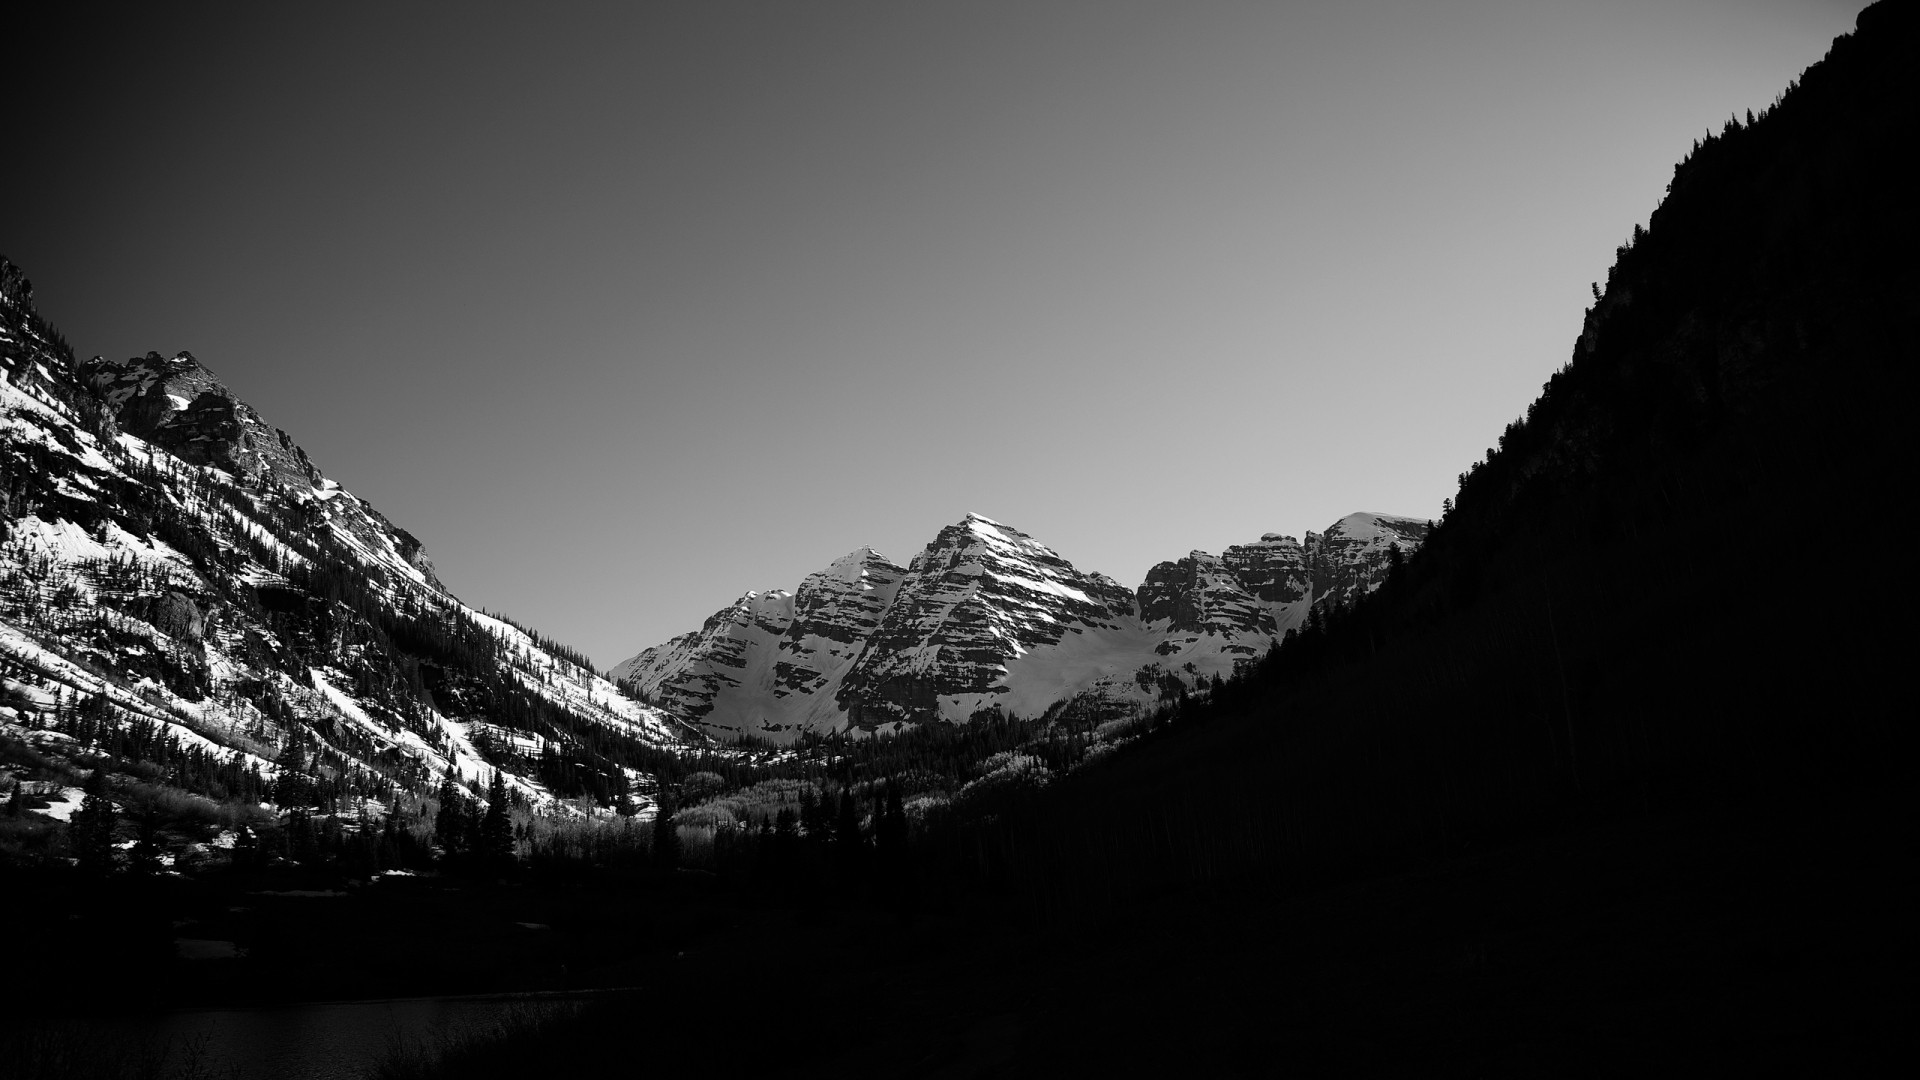
\includegraphics[width=0.8\textwidth]{appendices/ref_mountain.png}
    \caption{Reference image for the image processing verification}
    \label{fig:ref_mountain}
\end{figure}

\section{Derivations} \label{app:derivations}
\subsection{Theoretical maximum throughput of VHDL solution} \label{app:derivations:theomax}

\begin{align}
    b  & = \frac{i_p}{t_t} \\
       & = \frac{i_w i_h}{t_i+(i_h-w_l+1)t_r} \\
       & = \frac{i_w i_h}{(\frac{i_w}{b_e}+d_l)w_l+(i_h-w_l+1)(\frac{i_w}
       {b_e}+d_l)} \\
       & = \frac{i_w i_h}{(\frac{i_w}{b_e}+d_l)(i_h+1)} \\
       & = \frac{i_w i_h}{d_l(i_h+1)+\frac{i_w}{b_e}(i_h+1)} \\
       & \approx \frac{i_w}{d_l+\frac{i_w}{b_e}}
    \label{eq:theomaxb}
\end{align}
\begin{tabular}{rl}
    $b     =$ & theoretical throughput of VHDL solution \\
    $i_p   =$ & total image pixels \\
    $t_t   =$ & total processing time \\
    $i_w   =$ & image width \\
    $i_h   =$ & image height \\
    $t_i   =$ & time to send the initial lines \\
    $w_l   =$ & windows length \\
    $t_r   =$ & iterration time to process one line \\
    $b_e   =$ & ethernet throughput \\
    $d_l   =$ & delay between sending two image lines \\
\end{tabular} \\

\subsection{Theoretical maximum throughput of VHDL Wallis core} 
\label{app:derivations:theomaxvhdlwallis}

\begin{align}
    b  & = \frac{i_p}{t_w} &\\
       & = \frac{i_wi_h}{\frac{n_{ps}}{b_w}} &\\
       & = \frac{i_w i_h b_w}{w_l i_w (i_h-w_l+1)} &\\
       & = \frac{i_hb_w}{w_l (i_h-w_l+1)} &\\
       & = \frac{b_w}{w_l (1-\frac{w_l}{i_h}+\frac{1}{i_h})} &\\
       & \approx \frac{b_w}{w_l} &(i_h \to \infty)
    \label{eq:theomaxvhdlwallis}
\end{align}
\begin{tabular}{rl}
    $b     =$ & theoretical throughput of VHDL Wallis filter \\
    $i_p   =$ & total image pixels \\
    $t_w   =$ & total processing time of Wallis filter \\
    $i_w   =$ & image width \\
    $i_h   =$ & image height \\
    $n_{ps}=$ & Number of pixels processed by Wallis filter on input \\
    $b_w   =$ & throughput of Wallis filter \\
    $w_l   =$ & window length \\
\end{tabular} \\

\end{appendix}
\clearpage{\pagestyle{empty}\cleardoublepage}


% ==============================================================================
%
%                             B A C K M A T T E R
%
% ==============================================================================
\backmatter
\clearpage{\pagestyle{empty}\cleardoublepage}
% % Indexing: memman.pdf, pp. 302ff.
% \printindex
% %>>>
\newpage\null\thispagestyle{empty}\newpage
\end{document}

